\documentclass[journal,10pt,onecolumn,compsoc]{IEEEtran} 
    \usepackage[margin=0.75in]{geometry} 
    \usepackage{pdfpages} 
    \usepackage{graphicx}  
    \usepackage{changepage}
    \graphicspath{/images} 
    \usepackage[english]{babel}
    \usepackage{blindtext}
 
    \makeatletter
    \renewcommand{\paragraph}{\@startsection{paragraph}{4}{0ex}%
       {-3.25ex plus -1ex minus -0.2ex}%
       {1.5ex plus 0.2ex}%
       {\normalfont\normalsize\itshape}}
    \makeatother
    \stepcounter{secnumdepth}
    \stepcounter{tocdepth}
    
    \usepackage{tikz}
    \usetikzlibrary{shapes,arrows}
    \tikzstyle{block} = [rectangle, draw, fill=blue!20, 
    text width=5.5em, text centered, rounded corners, minimum height=4em]
    \tikzstyle{subblock} = [rectangle, draw, fill=blue!20, 
    text width=7em, text centered, rounded corners, minimum height=2em]
    \tikzstyle{datablock} = [rectangle, draw, fill=red!20, 
    text width=7em, text centered, rounded corners, minimum height=2em]
    \tikzstyle{line} = [draw, -latex']  
    
    \newenvironment{paddedtikzpicture}{\vspace*{0.5cm}
    \begin{center}\begin{tikzpicture}}
    {\
    \end{tikzpicture}\end{center}
    }  
    \setlength{\parskip}{\baselineskip} \setlength\parindent{24pt}
    \usepackage{url}
    \usepackage{setspace}
    \usepackage{geometry}
    \geometry{textheight=9.5in, textwidth=7in}
    \usepackage{hyperref}
    \usepackage{caption} 
    \usepackage{float} 
    \usepackage{rotating} 
    \usepackage{ragged2e} % provides \RaggedLeft
    \hypersetup{
        colorlinks,
        citecolor=black,
        filecolor=black,
        linkcolor=black,
        urlcolor=black
    }
    \geometry{textheight=9.5in, textwidth=7in}
    \usepackage{listings}
    \usepackage{color}
    \usepackage{cite}
    \definecolor{shadecolor}{RGB}{220,220,220}
    \lstdefinelanguage{JavaScript}{
        keywords={typeof, new, true, false, catch, function, return, null, catch, switch, var, if, in, while, do, else, case, break},
        keywordstyle=\color{blue}\bfseries,
        ndkeywords={class, export, boolean, throw, implements, import, this},
        ndkeywordstyle=\color{darkgray}\bfseries,
        identifierstyle=\color{black},
        sensitive=false,
        comment=[l]{//},
        morecomment=[s]{/*}{*/},
        commentstyle=\color{purple}\ttfamily,
        stringstyle=\color{red}\ttfamily,
        morestring=[b]',
        morestring=[b]"
      }
      \lstset{
        language=JavaScript,
        backgroundcolor=\color{shadecolor},
        extendedchars=true,
        basicstyle=\footnotesize\ttfamily,
        linewidth=7in,
        xleftmargin=.25in,
        showstringspaces=false,
        showspaces=false,
        numbers=left,
        numberstyle=\footnotesize,
        numbersep=9pt,
        tabsize=2,
        breaklines=true,
        showtabs=false,
        captionpos=b
     }
    
    % 1. Fill in these details
    \def \CapstoneTeamName{		The Dream Team}
    \def \CapstoneTeamNumber{		57}
    \def \GroupMemberOne{			Daniel Schroeder}
    \def \GroupMemberTwo{			Aubrey Thenell}
    \def \GroupMemberThree{			Parker Bruni}
    \def \CapstoneProjectName{		A Scalable Web Application Framework for Monitoring Energy Usage on Campus  }
    \def \CapstoneSponsorCompany{	Oregon State Office of Sustainability}
    \def \CapstoneSponsorPerson{		Jack Woods}
    
    % 2. Uncomment the appropriate line below so that the document type works
    \def \DocType{		%Problem Statement
            %Requirements Document
            %Technology Review
            % Design Document
            %Progress Report
            }
            
    \newcommand{\NameSigPair}[1]{\par
    \makebox[2.75in][r]{#1} \hfil 	\makebox[3.25in]{\makebox[2.25in]{\hrulefill} \hfill		\makebox[.75in]{\hrulefill}}
    \par\vspace{-12pt} \textit{\tiny\noindent
    \makebox[2.75in]{} \hfil		\makebox[3.25in]{\makebox[2.25in][r]{Signature} \hfill	\makebox[.75in][r]{Date}}}}
    % 3. If the document is not to be signed, uncomment the RENEWcommand below
    %\renewcommand{\NameSigPair}[1]{#1}
    
    %%%%%%%%%%%%%%%%%%%%%%%%%%%%%%%%%%%%%%%
    \title{Final Report for: \linebreak Scalable Web Application Framework for Monitoring Energy Usage on Campus}
    \author{Daniel Schroeder, Aubrey Thenell, Parker Bruni \linebreak Group 57}
    \date{\today}
    
    \begin{document}
    \maketitle
    \vspace{2cm}
    \begin{center}
    \noindent \textbf{Abstract} \\
                \indent The purpose of this document is to provide final documentation for Group fifty-seven's capstone project. 
    \end{center}         
    
    \newpage
    \pagenumbering{arabic}
    \tableofcontents
        
    % 8. now you write! 
    \section{Introduction to Project}  
    \subsection{Why is this project important?}
    \indent As the population of the world grows exponentially, the demand for energy grows with it. Unfortunately, a massive source of energy for humans comes from non-sustainable fuel burning. This burning releases greenhouse gasses into the earth’s atmosphere, which results in the heating of our planet and many consequences that come as a result. To combat this, communities have decided that it is time to get our energy from more sustainable sources, as well as use it in more sustainable ways. In order to be more sustainable and conscious of our energy consumption, we need to implement modern tools to monitor energy usage data and use that data to make informed decisions on future infrastructure projects. This is necessary to reduce our carbon footprint, reduce costs, and move society to a more sustainable (and eventually fully sustainable) future in regards to energy consumption.

    \indent Oregon State University is revered for its energy efficiency and sustainability and is committed to reducing its carbon footprint through renovations and sustainable consideration with new projects. In this era of technology it is necessary to utilize the tools that are available to us when designing and implementing systems that will increase energy efficiency. Oregon State focuses on reducing its overall costs while supporting a more sustainable environment through less consumption and emissions. With this in mind, OSU has installed energy meters in campus buildings to monitor and record energy data so that it may be analysed by members of Oregon State University’s Sustainability Office. The data that is gathered from these systems can be used to make educated decisions about the current energy usage systems in place, such as monitoring strange fluctuations or anomalies in energy usage in any given building. OSU can address and correct any potential waste from occurring as well as provide a foundation of knowledge to reference when planning future infrastructure projects by utilizing these systems.
    \subsection{Who requested it?}
    \indent Oregon State University's Office of Sustainability previously had contracted a company Lucid to create a web application that acted as an administrative dashboard for monitoring energy use across campus. However, as Oregon State University Sustainability Office scales up its operations and automated reporting, the price of Lucids contract becomes exponentially expensive to maintain. In order to continue data aggregation efforts, the Oregon State Sustainability office has recognized an opportunity for our team to create and plan a project that can take the place of the legacy system. Through creating an EECS capstone project, the Office of Sustainability was able to have an internally sourced web application that can be modified to whichever specifications they desire. It will also save the University hundreds of thousands of dollars that was previously spent on Lucid's services and direct that money towards more sustainable projects for the entire University and help Oregon State reach its carbon neutrality goal of 2025.
    \subsection{Meet the team}
    %%%%% answers the prompts: 
    % Who are the members of your team? 
    % What were their roles?
    % What was the role of the client(s)?} (I.e., did they supervise only, or did they participate in doing development
    \subsubsection{Daniel Schroeder - Developer}
    Daniel was responsible for generating a lot of the front-end data binding implementations with AngularJS. He implement the majority of functionality for all of the main components of the application (blocks, dashboards, stories, buildings). A lot of this process involved finding intuitive ways to query for aggregated data and populate web forms or UI components according to what is needed. A majority of Daniel's contributions revolved around generating a lot of Bootstrap4 and AngularJS webpages that auto-populated drop-down menus, graph data, or user objects so the user could view, create, edit, and delete all of the major components of the application. Additionally, Daniel needed to write route handler functions for and Express.js app that aggregated certain datasets and returned the correct data to the client. 
	\subsubsection{Aubrey Thenell - Developer}
	Aubrey was responsible for most of the backend based code. Specifically, she was responsible for the data collection server. This contribution allows data storage into the database, which is retrieved by the web application. She was also responsible for all email based functionality of the website. This includes invitation emails, high energy usage detection emails, and down meter emails. She was also responsible for a lot of the security based functionality. This includes all form validation to ensure malicious injection won't affect the database. It also includes sitewide permissions authentication. This ensures that people don't access things they shouldn't have access to. Aubrey also wrote the interface for the built in Kilowatt Crackdown Challenge that the Office of Sustainability runs annually. Finally, Aubrey contributed by documenting all of the code with JSDocs.
	\subsubsection{Parker Bruni - Developer}
	
	Parker was involved in designing the UI and overall look and feel of the application, as well as formatting many of the elements within the site. He used methods of CSS and Bootstrap as well as knowledge of what makes a web application appealing to a user to give the site a clean and modern feel by use of color schemes and minor site animations. He also implemented the initial stages of charting using chart.js and implemented the google maps API that is found on the home page. 
	
	\subsection{Role of the Client}
	Our client, Jack Woods, is a student at Oregon State University who is employed by the Office of Sustainability. He served as a direct line of communication between our development team and the Office of Sustainability. He worked very closely with the team on development having regular meetings and was involved in team discussions online. As well as communication, Jack has contributed to the project in other ways, such as setting up our EC2 instance so our site may be publicly accessible as well as working with the team on code to insure correct functionality of some components.
	
    \section{Requirements Document}
    %%%%%%% ---------------------------------
    % Insert the requirements document
    %%%%%%% ---------------------------------
    \subsection{Introduction}

    \subsubsection{Purpose}
    The purpose of this document is to outline the project and all associated information. Furthermore, it will outline how the end product will be used, how it was developed, and all resources and documentation referenced and used during development. This document will also describe the application’s target audience, user interface, and any hardware/software requirements. Finally, it will define how our client, team, and users will see the final product and related functionality.
    \subsubsection{Scope}
    This project will provide a web application that displays different collections of energy use reports for campus buildings. Each of these collections will be customizable, with the ability to add, remove, and filter building data according to user preference. The web application will allow users to visually comprehend energy data in a way that can raise awareness about consumption and reduce the campus-wide carbon footprint. The web application will also have three different permission levels: Guest, Registered Users, and Admin Users. Each one will provide permissions to what can be viewed and edited.

    \subsubsection{Definitions, acronyms, and abbreviations} \label{definition}
    \begin{table}[h]
    \centering
    \begin{tabular}{ll}
    \textbf{Term} & \textbf{Definition} \\
    OSU & Oregon State University \\
    MEAN stack & MongoDB, Express, AngularJS, Node.js \\
    JSON & JavaScript Object Notation \\
    AcquiSuite & Data Acquisition Servers responsible for metering energy usage \\
    Collections & User Interface dashboard that displays assortment of blocks \\
    Blocks & Charts/graphs of building data \\
    Stories & Collections of dashboards 
    \end{tabular}
    \end{table}
    \subsubsection{References} 
    The references are:
    \begin{itemize}
        \item AcquiSuite and Modbus Information \cite{aquisuite_emb} \cite{modbus_practices} \cite{modbus} \cite{AcquiSuite}
        \item D3.js \cite{d3_home}
        \item Vis.js \cite{vis}
        \item The M.E.A.N. Stack \cite{mean}
        \item JSON \cite{json}
        \item BuildingOS \cite{BuildingOS}
        \item Mocha.js \cite{mochajs}
    \end{itemize}
    
    \normalsize
    \subsubsection{Document Overview}
	The remaining sections of this document provide a more elaborate description of product functionality, assumptions, and specific requirements. Section 2 provides information about functional requirements, data requirements, and assumptions made for designing the \textit{Scalable Web Application Framework for Monitoring Energy Usage on Campus}. Section 3 outlines the specific requirements for the final product, the external interfaces that communicate with the software, and the functional requirements of the system.
	
    \subsection{Overall description}
    This section will provide an overview of the web application as a whole, including:
        \begin{enumerate} 
            \setlength\itemsep{1mm}
            \item Details about the user interface and expected user interactions.
            \item An outline of specific constraints and dependences included in development. 
            \item Background information about the specific software requirements.
        \end{enumerate}
    \subsubsection{Product perspective}
    %A block diagram showing the major components of the larger system, interconnections, and external interfaces can be helpful.
    %5.2.1.1 System interfaces
    %This should list each system interface and identify the functionality of the software to accomplish the system
    %requirement and the interface description to match the system.

    This product will replace the current web application that is used by The Oregon State Sustainability Office. The product will display energy usage information about Oregon State University buildings through an intuitive user interface. The application will gather data from energy meters by connecting to AcquiSuite\texttrademark data acquisition servers. The energy data from the meters will be transferred to a database that the product will access directly. Users will interact with the application interface from an internet browser application. 
    
    \subsubsection{Product functions}
    The product will allow users to create accounts that may be given either administrative or user permissions. Users have the ability to personalize their accounts. Administrators accounts will have special capabilities that user accounts will not. \\
    The application will allow users to create customizable dashboards that will contain easily adjustable “blocks” of campus building data that will contain the campus building energy usage data. These “blocks” of data will be the basic building blocks for the dashboard and will provide an intuitive view of the data. They will feature various graph types, building energy efficiency rankings, and data trends.\\
    Each OSU building that contains the energy monitoring meter(s) will have a specific, non-customizable page that will display general information. The product will also have a public interface and a private administrative interface.\\
    Administrators of the application will have the ability to add, remove, or edit entire buildings profiles, building subspaces, or individual meters.
    
    \subsubsection{User characteristics}
    A user that will be using the general public UI will not need to know any specific information about the application to navigate the various energy data presentations. A public user will be able to intuitively navigate the UI at their discretion. \\ 
    An administrative level user will need a basic understanding of the tools of the application because they will be allowed the freedom to control parts of the website as well as have access to more specific energy data within the application. An administrator will likely not need extensive training to use this application for more specific purposes as the administrator UI will be designed to be intuitive to navigate.
    \subsubsection{Constraints}
    Data updates will be limited to a granularity of 15 minute intervals. The data acquisition server is capable of providing a granularity of up to 15 second intervals but it is not necessary for the purposes of the application. Any other constraints on the product are subject to the internet browsing interface that is accessing our product. The UI will be intuitive and able to navigate data presentations, but will not allow manipulation of the data or underlying structure of the application.
    
    \subsubsection{Assumptions and Dependencies}
    The application will be dependant on the data acquisition server. If the data acquisition server is drastically changed or removed, the application will not be functional. Meter data within the application will also be limited by the functionality of the meters themselves. Should a meter malfunction, the energy data will not be gathered which may cause some of the data presentations to deviate from expected data. The use of the application will require a compatible web browsing interface, which may be limited to browsers such as Firefox, Chrome, and Internet Explorer. The functionality of the product will depend on those internet browsers performing as expected with regards to their intended functionality and internet access. 

    \subsubsection{Apportioning of Requirements}
    Future versions of the application may include features such as cost tables, automated electronic invoice generation, energy billing analysis capabilities, budget analysis capabilities, and mobile energy data entry.
    
    \subsection{Specific Requirements}
    
    \subsubsection{External Interfaces}
    AcquiSuite data acquisition servers [meters] made by Obvious
    \begin{itemize}
        \setlength\itemsep{1mm}
        \item Used for collecting electric, water, gas, steam, and other energy parameters over the web.
        \item Data is received through IP-based connection.
        \item Data can be reached anywhere with an internet connection, as long as the AcquiSuite is online.
        \item Data will be collected every 15 minutes.
        \item Data from the AcquiSuite servers will be stored into a database.
    \end{itemize}

    \subsubsection{Functions}
    This section defines how the software system should behave with regards to input and output.
    \begin{itemize}
        \setlength\itemsep{1mm}
        \item The system shall receive and store data from AcquiSuite data acquisition servers into the database. 
        \item The system shall have input validation measures in place to monitor incoming data and protect from malicious injections.
        \item The system shall retrieve data from the database and populate webpages with filtered datasets when prompted.
        \item The system shall have permission based restrictions for accessing certain data.
        \item The system shall generate alerts for offline buildings and high energy usage.
        \item The system shall generate emails for users to access a sign-up form and create an account.
        \item The system shall be able to create arbitrary combinations of datasets given user filters.
        \item The system shall be able to calculate rankings for all the buildings based on certain metrics like ``kilowatt-hour consumption''.
    \end{itemize}

    \subsubsection{Performance Requirements}
    This section describes the functionality requirements for the software as well as what a user should be able to accomplish when using the web application.

    \paragraph{Users}
    The system will have 3 types of users: admin level users, registered users, and generic users. An administrative user will be able to add new meters, buildings, and other objects into the database. A registered user, for example the head of a department, can create their own stories with information and collections that are unique to their own interests or departments. Lastly, a generic user can simply view the publically facing web application and see public dashboards and browse public stories. 
    \begin{itemize}
        \setlength\itemsep{1mm}
        \item A registered user should be able to customize dashboard layouts in a grid-based orientation. A \hyperref[definition]{\textit{story}} page should have a customizable layout where a user can add different \hyperref[definition]{\textit{blocks}} with information relevant to their personal needs.
        \item An administrative user should be able to add buildings to the database through a web form.
        \item An administrative user should be able to add data aquisitions servers.
        \item An administrative user should be able to download specific datasets as a .csv file.
        \item An administrative user should be able to customize public stories.
    \end{itemize}

    \paragraph{Data Management}
    \begin{itemize}
        \setlength\itemsep{1mm}
        \item The web application should update data blocks every 15 minutes as new data is received into the database.
        \item The web application should allow users to create  which are collections of dashboards. These 
        \hyperref[definition]{\textit{stories}} are meant to bring related buildings and datasets together into intuitive groups, for instance ``Residence Halls'' or ``Engineering Buildings.''
        \item The application should be able to filter building data by date range specifications.
        \item The web application should be able to scale up to as many buildings are on campus.
        \item The web application should properly create and store new entities (buildings, users, meters) into the database.
        
    \end{itemize}    

    \paragraph{Visualization}
    \begin{itemize}
        \setlength\itemsep{1mm}
        \item The web application should be able to generate different types of graphs for different \hyperref[definition]{\textit{blocks}}. For example load-profile charts, comparative line charts, and heat maps.
        \item The web application should have generic pages for each building in the database. This page will display a series of graphs and charts that outline energy usage for a particular building.
        \item The \hyperref[definition]{\textit{blocks}} on each page should automatically update as new data is received by the database.
    \end{itemize}
    \paragraph{Objects}
        The system should have three main entities: 
        \begin{itemize}
            \setlength\itemsep{1mm}
            \item \textbf{Building} - A building on campus that is connected to a data acquisition server.
            \item \textbf{Meter} - A specific data acquisition server.
            \item \textbf{User} - A user with a specific role.
        \end{itemize}
        
    \subsubsection{Logical Database Requirements}
    Most of the calls to the database will be requests for meter data from a specific building or group of buildings. Access to the database should be hidden from the user and only accessed from the back-end of the application itself. Any input into the database should be validated and encrypted, if applicable. 
    
    \subsubsection{Design Constraints}
    Design constraints may include server availability which could harm scalability.
    \paragraph{Standards Compliance}
    There may be standards when storing energy data based on The Office of Sustainability Standards.
    [Check with Client]

    \subsubsection{Software System Attributes}
    
    \paragraph{Reliability}
    The system will be reliable at the time of deployment if all data displayed in graphs and charts is correct.
    \paragraph{Availability}
    The system should be consistently available as long as the servers are up and running. As a web application, the system will be available via URL.
    \paragraph{Security}
    The system will validate input for duplicate and malicious content.
    The system will also have back-end functionality to protect user passwords through proper hashing.
    The web application will restrict access to certain pages and content based on user roles and permissions.

    \paragraph{Maintainability}
    Maintainability for this application should be simple for anyone with web development experience. The application code will be organized into logical directories and sub directories that should mimic a full stack web application. There will be documentation that explains how to connect to the AcquiSuite servers and how to use our API for data collection.
    \paragraph{Portability}
    Our web application should be visible and accessible from most web browsers. There are not any host-dependent constraints since it will be hosted from a central server and available to the public via the internet. The source code should stay on Github so modifications can be made easily.
    


include the original document, showing what you thought, at the time, was the project definition with the original Gantt chart
Add (your client should have okay'd): What new requirements were added? What existing requirements were changed? What existing requirements were deleted? Why? 
Add: Final Gantt Chart as a record of what happened when.
    
    \section{Design Document}
    \subsection{Introduction}
\subsubsection{Purpose}

The purpose of this Software Design Document (SDD) is to provide details about the architecture of the web application as well
as details about each component. It will describe the underlying design of each component and their purpose within the context
of the application that will allow Oregon State affiliates to effectively monitor energy usage on campus.

\subsubsection{Scope}

The software outlined in this document will function as an interface by which Oregon State students, faculty, and affiliates
may monitor energy usage of various buildings located on the Oregon State Campus. It will act as a tool for users to 
make informed infrastructure decisions and adjustments or act as a display piece to be presented within buildings on campus.
It will serve the OSU Office of Sustainability as a replacement to an outdated and costly implementation. 

\subsubsection{Overview}
Oregon State University is constantly making strides to reduce its carbon footprint and reduce its energy consumption. There is a carbon neutrality goal for 2025 where the university is trying to generate as much energy as it uses and have a net carbon footprint of zero. Our web application aims to monitor the energy use of buildings on campus in order to create a visual representation of each building's consumption and incentivize people to monitor their consumption habits and reduce the campus's overall consumption.

\noindent Our web application will resemble an administrative dashboard with charts and graphs of energy use over time for individual buildings and subgroups of buildings on Oregon State's campus. 
Our application will have a series of public facing pages that will show energy usage for all the buildings on campus that have AcquiSuite meters as well as display user generated stories of personalized dashboards. Each page will be a grid-based dashboard with personalized blocks for displaying data through time-series charts or graphs. A user will be able to add different blocks to create unique dashboards for their own unique interests and subsets of buildings. An example of this would be a dashboard designated to only residence halls where each block shows a usage over time graph for energy consumption of each residence hall. Users will be able to apply date filters to their blocks to generate different data sets and more explicit visualizations.

\noindent Our web application will be constructed using a MEAN Stack framework hosted on AWS. Our application will have a MongoDB database server and a Node.js application server hosted on a single virtual EC2 instance to make deployment easy and reliable.

\subsubsection{Reference Material} 
    \begin{itemize}
        \item Bootstrap4 Dashboards \cite{dashboard_bootstrap} 
        \item Using OAuth 2.0 to Access Google APIs \cite{oauth} 
        \item Data-Driven Documents \cite{data_driven}
        \item AngularJS \cite{ng}
        \item AcquiSuite by Obvius \cite{AcquiSuite}
    \end{itemize} 
\subsubsection{Definitions and Acronyms}
This subsection will define terms and acronyms that are specific to the application that may otherwise be misunderstood or poorly interpreted.
\begin{itemize}
    \item \textbf{Dashboard:}
        A grid-based information management tool for visually tracking and displaying metrics and data through graphs and charts.
    \item \textbf{Block:} 
        An individual graph or chart depicting time-series data. More specifically, it is an HTML element containing one or more buildings, with filter buttons, informative text, and graphs.
    \item \textbf{Story:} 
        A user generated collection of dashboards. What each story displays is based solely on user preferences. With multiple stories, the user can select between ``presets'' that can show different dashboards.
    \item \textbf{MEAN Stack:} 
        An acronym used to define a full stack application engineered from the MongoDB, Express.js, Angular.js, and Node.js frameworks. 
    \item \textbf{Bootstrap:} 
        Bootstrap CSS is a front-end framework that uses component templates to easily generate different HTML elements like buttons, navigation, or forms. 
    \item \textbf{OAuth 2.0:} 
        OAuth 2.0 is an authorization protocol that grants authentication through tokens rather than credentials. 
    \item \textbf{Filter:} 
        Filters are essentially parameters for fetching data from that constrain the subset of data being received to the specifications of the filter parameters (i.e. a date range). 
    \item \textbf{D3:} 
        D3.js is a visualization framework that appends charts and graphs to DOM elements on a webpage. 
    \item \textbf{AcquiSuite:} 
        AcquiSuites are data acquisition servers made by a company called Obvius that post building meter data to a designated IP address.
    \item \textbf{AWS:} 
        AWS is an acronym for Amazon Web Services which offers reliable cloud computing services for building and hosting web applications.
   \item \textbf{Passport:} 
        Passport is authentication middleware for Node.js. Extremely flexible and modular, Passport can be unobtrusively dropped in to any Express-based web application. A comprehensive set of strategies support authentication using a username and password, Facebook, Twitter, etc.
\end{itemize}
\subsection{System Overview} 
Our web application will provide users with the functionality to create unique dashboard-style collections of charts and graphs to analyze energy use from Oregon State's campus buildings. Our system will be highly modular, containing multiple smaller components that provide their own individual functionality while sharing information across other components. Designing a modular architecture will simplify the code base and allow the developers to encapsulate specific data models as their own entities and keep abstractions in the system differentiable.

\noindent Our design also stems from the main constructs behind AngularJS and data injection. Most of our components and subsystems are, at large, data models and objects that hold all the necessary information to create graph and charts. With this design, AngularJS services will extract data from the session user and rendered components and generate render the desired graphs and views to the content container. This allows the application to break up back-end services as well as UI components to simplify how data is gathered and processed.
\subsection{Design Viewpoints and Concerns}
\subsubsection{Stakeholders and Concerns}
Developers concerns consist of simplifying complex model functions, replicable components, modular subsystems, and simple data access functionality. Addressing and capitalizing on these concerns will create an application design that will enhanced understanding, simplify implementation, and produce a high-end product. From a developer's standpoint, it is also essential to design an application that is ideal for both implementation and usability.

\noindent Client concerns revolve around satisfying the requirements of the application and providing all the necessary user functionality. The implementation should adhere to the client's requests and specifications while creating a user-friendly interface to perform all the necessary actions.
\subsubsection{Design Viewpoints}
\paragraph{Context Viewpoint}
The design of this web application will greatly depend upon satisfying the user actions outlined in the requirements document. With that in mind, all components and subsystems should cater towards simplifying the user's experience while performing actions and navigating through the application. This viewpoint provides design constraints for individual component functionality, as well as the overall layout and structure of the application as a whole. Our design implementations should cater to a wide range of users while creating an elegant way for the user to create, edit, and remove content.
\paragraph{Composition Viewpoint}
This application contains a number of components that are recurrently used throughout the application and across users. These include the basic data blocks, dashboards, and stories that a user can create. The design of this application should embrace the modularity of these components and provide a consistent model for individual functionality while maintaining the ability to communicate and pass data across different components or objects. 

\paragraph{Dependency Viewpoint}
With a design focused around modularity and individualized components, there needs to be designs for services and dependencies so each component can interact. Some examples of these are: how a block component depends on multiple entities contained inside the block object like the building objects stored within the block, the filter's current values, the graph template, and the graphing service. The design of this application should encapsulate the relationships between different modular components and provide intuitive means for inter-component communication.

\paragraph{Information Viewpoint}
Our applications design should provide logical ways of storing data and receiving data from building meters. This involves an explicit declaration of individual data models and how how data is created and stored. Our design will attempt to create a modular data structure where data specific to certain entities reside in the entity objects themselves. This allows the application to access data from an individual component as it gets created or moved throughout the application.

\paragraph{Logical Viewpoint}  
The application should maintain a consistent model for each component which can be used in different ways for different purposes. An entity should contain and provide the necessary information as it is needed throughout various areas of the application. The design of the application as a whole should consider where certain data is needed, and what data models must be present to satisfy the system's requests.
\begin{figure}[H]
    \centering
    \includegraphics[width=14cm]{images/CapstoneUML.eps}
    \caption{A UML diagram to show component relationships.}
\end{figure}
\paragraph{Interface Viewpoint}  
Users will require a front end interface to interact with the application and utilize its functionality. The design of these interfaces should focus on satisfying all user actions in a simple and appealing manner. Users should be able to intuitively navigate the application and perform essential tasks without confusion or error.
\paragraph{Structure Viewpoint} 
The design of this application describes the structure of independent modular components and their relationships to other entities. From a developer's standpoint, organizing the structure and interdependence of different components is essential when implementing a complex system. This application's design highlights key individual components along with their individual functionality and relationships with other entities. 
\paragraph{Interaction Viewpoint}  
Each object component in the application should not need any logic to handle its interactions with other components. This functionality should be performed by services and model functions implemented in the back-end of the application. The design of this application aims to keep data and entities separate from the logical functionality required to extract and share data across different components.
\subsection{System Architecture}
\subsubsection{Architectural Design}

\begin{figure}[H] 
\begin{paddedtikzpicture}[node distance = 2cm, auto]
    % Place nodes
    \node (ui)[block] {User Interface}; 
    \path (ui.east)+(2,5) node (nav) [block] {Navigation}; 
    \path [line] (ui)+(-0.3,0.7) -- (nav);
    \path (ui.east)+(2,3) node (block) [block] {Create Block}; 
    \path [line] (ui) -- (block);
    \path (ui.east)+(2,1) node (dash) [block] {Create Dashboard}; 
    \path [line] (ui) -- (dash);
    \path (ui.east)+(2,-1) node (story) [block] {Create Story}; 
    \path [line] (ui) -- (story);
    \path (ui.east)+(2.35,-3) node (add) [block,  text width=7.5em] {Add Building/Meter};
    \path [line] (ui) -- (add);
    \path (ui.east)+(2,-5) node (log) [block] {Log In}; 
    \path [line] (ui)+(-0.3,-0.7) -- (log);
    
    %Create Dashboard
    \path (nav.east)+(2,0) node (select) [subblock] {Get User Selection};
    \path [line] (nav) -- (select);
    \path (select.east)+(2,0) node (route)[datablock] {Pass Selected Route to View};
    \path [line] (select) -- (route); 
     
    %Create Block
    \path (block.east)+(2,0.5) node (ctype) [subblock] {Get Chart Type};
    \path [line] (block) -- (ctype);
    \path (block.east)+(2,-0.5) node (bdata)[subblock] {Get Building Data};
    \path [line] (block) -- (bdata); 
    \path (block.east)+(5,0) node (template)[subblock] {Retrieve Graph Template}; 
    \path [line] (bdata) -- (template); 
    \path [line] (ctype) -- (template); 
    \path (template.east)+(2,0) node (d3)[subblock] {Build D3}; 
    \path [line] (template) -- (d3); 
    %Create Dashboard
    \path (dash.east)+(2,0) node (getblocks) [datablock] {Get Blocks};
    \path [line] (dash) -- (getblocks);
    \path (getblocks.east)+(2,0) node (saveblock)[datablock] {Add Blocks to Dashboards};
    \path [line] (getblocks) -- (saveblock); 
    %Create Story
    \path (story.east)+(2,0) node (createdash)[datablock] {Get Dashboards};
    \path [line] (story) -- (createdash); 
    \path (createdash.east)+(2,0) node (adddash)[datablock] {Add Dashboards to Story};
    \path [line] (createdash) -- (adddash); 
    
    %Add Building
    \path (add.east)+(2,0) node (input)[subblock] {Get Input Data};
    \path [line] (add) -- (input); 
    \path (input.east)+(2,0) node (storeinput)[subblock] {Store Input Data};
    \path [line] (input) -- (storeinput); 

    %Log In
    \path (log.east)+(2,0) node (auth) [subblock]  {Google oAuth 2.0};
    \path [line] (log) -- (auth);
    \path (auth.east)+(2,0.5) node (store) [subblock] {Store User};
    \path [line] (auth) -- (store);
    \path (auth.east)+(2,-0.5) node (retrieve)[subblock] {Retrieve User}; 
    \path [line] (auth) -- (retrieve);
\end{paddedtikzpicture}
\caption{An overview of the major application systems.} 
\end{figure}
\subsubsection{Decomposition Description}

All database operations (retrieving data and storing data) are denoted with red fill and will be carried out by an AngularJS ``Service'' within the component's controller. 
\paragraph{Log In}
\begin{figure}[H] 
\begin{paddedtikzpicture}[node distance = 2cm, auto]
    % Place nodes
    \node (login)[block] {Log In}; 
    \path (login.east)+(2,0) node (googleauth) [block] {Contact Google oAuth API}; 
    \path [line] (login) -- (googleauth);
    \path (googleauth.east)+(2,0.5) node (store) [datablock] {Store User in Database}; 
    \path [line] (googleauth) -- (store);
    \path (googleauth.east)+(2,-0.5) node (retrieve) [datablock] {Retrieve User From Database}; 
    \path [line] (googleauth) -- (retrieve);
\end{paddedtikzpicture} 
\caption{A functional representation of the log in subsystem.} 
\end{figure}
\paragraph{Navigation} 
\begin{figure}[H] 
\begin{paddedtikzpicture}[node distance = 2cm, auto]
    % Place nodes
    \node (nav)[block] {Navigation Bar}; 
    \path (nav.east)+(2,0) node (route) [block] {Get Route from Nav Item}; 
    \path [line] (nav) -- (route);
    \path (route.east)+(2,0.5) node (pass) [subblock] {Pass Route to Parent Scope}; 
    \path [line] (route) -- (pass);
    \path (route.east)+(2,-0.5) node (view) [datablock] {Call Route's Get Function}; 
    \path [line] (route) -- (view);
    \path (route.east)+(5.5,0) node (render) [subblock, text width=8em] {Render New View HTML}; 
    \path [line] (pass) -- (render);
    \path [line] (view) -- (render);
\end{paddedtikzpicture} 
\caption{A functional representation of the navigation subsystem.} 
\end{figure}
\paragraph{Create Block} 
\begin{figure}[H] 
\begin{paddedtikzpicture}[node distance = 2cm]
    % Place nodes
    \node (create)[block] {Create Block}; 
    \path (create.east)+(2,0) node (view) [block] {Serve Web Form in View};
    \path [line] (create) -- (view);
    \path (view.east)+(2,0.5) node (charts) [datablock] {Pull Charts from Database}; 
    \path [line] (view) -- (charts);
    \path (view.east)+(2,-0.5) node (buildings) [datablock] {Pull Buildings from Database}; 
    \path [line] (view) -- (buildings);
    \path (view.east)+(5.5,0) node (submit) [subblock, text width=8em] {Get User from Data}; 
    \path [line] (charts) -- (submit);
    \path [line] (buildings) -- (submit);
    \path (submit.east)+(2,0) node (store) [datablock, text width=8em] {Store Block in User Object}; 
    \path [line] (submit) -- (store);
\end{paddedtikzpicture} 
\caption{A functional representation of the block creation subsystem.} 
\end{figure}
\paragraph{View Blocks}
\begin{figure}[H] 
\begin{paddedtikzpicture}[node distance = 2cm]
    % Place nodes
    \node (view)[block] {View Blocks}; 
    \path (view.east)+(2,0) node (retrieve) [datablock] {Retrieve Blocks from User Object};
    \path [line] (view) -- (retrieve);
    \path (retrieve.east)+(2,0) node (render) [subblock] {Render Blocks to Content View}; 
    \path [line] (retrieve) -- (render);
    \path (render.east)+(2,0.5) node (edit) [datablock, text width=8em] {Edit Block Fields}; 
    \path (render.east)+(2,-0.5) node (delete) [datablock, text width=8em] {Delete Block};
    \path [line] (render) -- (edit);
    \path [line] (render) -- (delete); 
\end{paddedtikzpicture}  
\caption{A functional representation of the block view subsystem.} 
\end{figure}
User created blocks will be stored in their respective ``Blocks'' array This allows a user to keep track of the specific blocks they create and reuse them to create stories.
\paragraph{Create Dashboard}
\begin{figure}[H] 
\begin{paddedtikzpicture}[node distance = 2cm]
    % Place nodes
    \node (view)[block] {Create Dashboard}; 
    \path (view.east)+(2,0) node (retrieve) [datablock] {Retrieve Blocks from User Object};
    \path [line] (view) -- (retrieve);
    \path (retrieve.east)+(2,0) node (render) [datablock] {Store Selected Blocks in Dashboard Object}; 
    \path [line] (retrieve) -- (render);
    \path (render.east)+(2,0) node (edit) [datablock, text width=8em] {Store Dashboard in User Object};  
    \path [line] (render) -- (edit); 
\end{paddedtikzpicture}  
\caption{A functional representation of creating a dashboard object from user created block.} 
\end{figure}
A dashboard is a collection of blocks. The dashboard component provides a way to group blocks together based on user preference and display them in the content view by simply rendering each block stored.
\paragraph{Create Story}
\begin{figure}[H] 
\begin{paddedtikzpicture}[node distance = 2cm]
    % Place nodes
    \node (story)[block] {Create Story}; 
    \path (story.east)+(2,0) node (retrieve) [datablock] {Retrieve User Dashboards};
    \path [line] (story) -- (retrieve);
    \path (retrieve.east)+(2,0) node (add) [datablock, text width=8em] {Save Selected Dashboards to Story};
    \path [line] (retrieve) -- (add);
    \path (add.east)+(2,0) node (store) [datablock, text width=8em] {Store Block in Story Object};
    \path [line] (add) -- (store); 
\end{paddedtikzpicture}   
\caption{A functional representation of the story creation subsystem.} 
\end{figure}
Stories are stored in the User object who created them in an array ``Stories.'' This allows the application to render stories created by the session user easily and will eliminate the use of SQL style querying to retrieve stories based on a user key.
\paragraph{Add Building/Meter}
\begin{figure}[H] 
    \begin{paddedtikzpicture}[node distance = 2cm]
        % Place nodes
        \node (add)[block, text width=8em] {Add Building/Meter}; 
        \path (add.east)+(2,0) node (render) [subblock] {Render Input Form};
        \path [line] (add) -- (render);
        \path (render.east)+(2,0) node (store) [datablock, text width=8em] {Store Form Values As New Object};
        \path [line] (render) -- (store);
    \end{paddedtikzpicture}   
    \caption{A functional representation for storing new building and meter objects to the database.} 
\end{figure}

\paragraph{Create Graph}
\begin{figure}[H] 
    \begin{paddedtikzpicture}[node distance = 2cm]
        % Place nodes
        \node (graph)[block] {Create Graph}; 
        \path (graph.east)+(2,0) node (get) [datablock] {Get Data from Parent Block};
        \path [line] (graph) -- (get);
        \path (get.east)+(2,0) node (fetch) [datablock, text width=8em] {Fetch Graph Template};
        \path [line] (get) -- (fetch);
        \path (fetch.east)+(2,0) node (render) [subblock, text width=8em] {Serve Graph to HTML};
        \path [line] (fetch) -- (render);
    \end{paddedtikzpicture}   
    \caption{A functional representation for building a graph in a block.} 
\end{figure}
To render a chart or graph to the webpage, our application will gather all the parameters from the block component that contains the graph (the building(s), the chart type, and the date range). The the graph component will then fetch a D3 template for its specific chart type, input the data from the block, and serve it to the dashboard. 

\paragraph{Get AcquiSuite Data}
\begin{figure}[H] 
    \begin{paddedtikzpicture}[node distance = 2cm]
        % Place nodes
        \node (data)[datablock] {Receive AcquiSuite Data}; 
        \path (data.east)+(2,0) node (parse) [subblock] {Parse Data to JSON Object};
        \path [line] (data) -- (parse);
        \path (parse.east)+(2,0) node (store) [datablock, text width=8em] {Store Data in Building Object};
        \path [line] (parse) -- (store);
    \end{paddedtikzpicture}   
    \caption{A functional representation for storing AcquiSuite data to a building object.} 
\end{figure}
Timestamped data entries from AcquiSuite Servers will be contained in their respective building objects from which the data was sent. Similar to the rational behind storing blocks in the user object that created them, each building will have an array of meter data sorted by timestamp. This will allow our application to use a service to retrieve the data for any graphs or charts directly from the buildings objects in the relative block. A graph service can then fetch the building data, apply filters (like date ranges), and pass it to a D3 graph to render. This minimizes the amount of total data to be parsed and collected by narrowing the data to the relative block.

\noindent [\textbf{Note:} Subject to change in later revisions. The methodology of how to receive data from  AcquiSuite data acquisition servers is still being designed.]

\subsubsection{Design Rationale}
The system's architecture revolves around a heavily modular system where individual components have their own functionality and are able to work cohesively with other components. The modular architecture also breaks up the back-end components into smaller services which simplifies functionality across the entire application.

\subsection{Component Design}
This subsection is designated to describing individual components in greater detail, including the type of element, designated functionality, and the reasoning behind their design. 
Overall, this subsection aims to provide an in-depth view of the application components and describe their individual roles in the application as a whole.
    \subsubsection{Block}
        A Block is a component in our application that will act as a container for a graph, filter options, and provide information about the data in the graph.
        \paragraph{Element} 
            A Block is an HTML element that uses the Bootstrap 4 ``card'' component for its design. It will have a title bar with the Block's name, then a content container split into a grid. 
            On the left, the Block will display the building(s) being graphed, contain a column of filter buttons, and display the D3 graph in the right column. 
        \paragraph{Functionality}
            The Block component neatly organizes data for the user by encapsulating the data, filters, and graph components into one container. 
            A Block needs to pull data from the ``building'' objects that it contains, gather data from any filters, and pass all this data into the correct graph template to generate a D3 graph. 
            There will be a service within the Block's AngularJS controller that will gather this data and pass the desired output to the dashboard.
        \paragraph{Rationale} 
            The Block component is an efficient way to create a reusable HTML template that can be reproduced throughout the application. 
            This provides a simple and consistent process for displaying graphs and data. Additionally, the block component yields a compact solution for organizing data from multiple sources. 
    
    \subsubsection{Dashboard}
        The dashboard component acts a way to store collections of block objects based on user preference.
        \paragraph{Element} 
            A dashboard is an object in the database that holds a collection of block objects.
        \paragraph{Functionality}
            The dashboard object is a way to conveniently package blocks together into groups so users can reuse the same groups or create unique collections of different blocks. 
            When ``viewing'' a dashboard, the application will simply iterate through the block objects and render them to the view container in a vertical list.
        \paragraph{Rationale} 
            The dashboard components provides a simple way to organize data keep track of user generated collections. 
            The dashboard component will work nicely with AngularJS to render an HTML element for every object in an array, which in this case are the blocks in the dashboard.

    \subsubsection{Login}
        The Login component is an HTML button that will allow users to login with a Gmail account by redirecting the user to Google's oAuth 2.0 API.
        \paragraph{Element}
            The Login function will be a button in the corner of the screen or somewhere in the navbar. The button will change to ``logout'' if the user is already logged in.
        \paragraph{Functionality}
            Clicking the Login component will redirect the user to our authentication service. 
            The application will use ``PassportJS'' as an authentication middleware which authenticates the user with Google oAuth 2.0 tokens and sets the req.user variable upon redirecting to the specified route. 
            Once a user is logged in, they will have access to additional application functionality and navigation items based on role.
        \paragraph{Rationale}
            From a developer standpoint, requiring users to login for certain features will make separation of privileges much easier. With authentication, users will also be able to have the convenience of Google SSO.

    \subsubsection{Navigation Bar}
        The Navigation bar is a commonly used UI feature that provides users the ability to navigate through different webpages of the application.
        \paragraph{Element}
            The navigation bar will be an HTML element with differentiable ``nav-items'' that render different views to the content view space. There will be a fixed-top navigation bar for generic item and a side bar navigation for more explicit functionalities such as admin controls. 
        \paragraph{Functionality}
            Clicking on a nav-item has one of two functionalities: 
            \begin{itemize}
                \item Redirects the user to a new webpage by having the route's get function perform a redirect.
                \item Renders a new view to the webpage by having the route's get function render a new HTML view.
            \end{itemize}
            The navigation bar shows which item is currently being served by changing the style of the active nav-item to be different than the rest.
        \paragraph{Rationale}
            From a user perspective, having a navigation bar to navigate around the main features is an extremely useful UI design decision. 
            From a design perspective, having a dedicated area to insert useful links is much more streamline than listing them. 
            The navigation bar is a very useful tool for serving different content to the view space statically.
    
    \subsubsection{Graph Component}
        Our application will contain a graph component that accepts a graph type and data as input and constructs a graph using the D3 visualization framework.
        \paragraph{Element}
            A graph component will be an SVG element, created with D3, that is served to the webpage inside of a block. 
        \paragraph{Functionality}
            The graph component's functionality involves gathering different input parameters from the parent block component, fetching a template based on the graph type, and creating a unique graph. 
            The graph component should have its own service to handle all the data organization and create a list of uniform parameters than can be passed to a D3 graph template.
        \paragraph{Rationale}
            Having a structure like this simplifies the act of generating graphs by having a series of templates that can be fed data in a specific format. 
            The graph service can take all the data and different filter parameters from the block object and format it into the right structure. 
            All the computationally heavy functionality is black-boxed in the graph service and keeps the functionality handled by the user and front-end at a minimal. 
            Another benefit provided by the graph component is that it can change the graph dynamically. 
            Our application may include filters in the block component like a date range or a filter to change the graphed variable, which can trigger the graph service to reconstruct the data and create a new graph to serve based on the applied filters.
    
        \subsubsection{Story}
        A story is a container for user dashboards to be stored and retrieved. A story is an abstract object that allows the user to create unique collections of dashboards with general theme or purpose.
        \paragraph{Element}
            A story will be an database object that contains collections of dashboards.
        \paragraph{Functionality}
            Each story will have a collections of dashboards. The number of dashboards in the collection will vary from story to story based on user preference.
    
    \subsubsection{Content View}
        The content view is a portion of the webpage where different views can be rendered to provide different content.
        \paragraph{Element} 
            The content view will be an HTML container that resides within the context of the webpage. The user will be able to change the content of the container by selecting different navigation items.
        \paragraph{Functionality}
            When the user clicks on a button or list on the side bar, it will pass a route to the scope variable in the view container. Once that route is called, the Angular function ``ng-include'' will inject the rendered HTML into the context of the webpage.
        \paragraph{Rationale} 
            From a developer standpoint, having a content view will dramatically reduce clutter both in the code and in the UI. The content view allows the application to serve dynamic content without reloading the webpage and creates a simple way to perform navigation services.



\subsection{Human Interface Design}
\subsubsection{Overview of User Interface}

\paragraph{Public User}
A public user is a user without a registered account or a user that is not logged in to their registered account. The authentication of a user is based on if 
they have a registered Oregon State Gmail domain. Public users will have limited access to features and data on the website. For example, the left side navigation
bar will be hidden from a public user. Public users will not be able to create personalized dashboards or stories. Public users will be allowed to view public 
user generated dashboards as well as general building dashboards. Essentially, public users will not be able to create personalized data sets or modify elements of the site but will be 
allowed to view general public data. 
\paragraph{Authorized User}
An authorized user is a user with a registered Oregon State Gmail account but does not have administrative privileges. When an authorized user is logged into their account, 
they have greater privileges than a public user as well as all privileges granted to a public user. They are allowed access to a left side navigation 
bar that has special functionality. Unique functionality granted by the vertical navigation bar include: viewing of personal and public dashboards, viewing of personal and public
stories, and access to personal settings. Authorized users may create personalized dashboards and stories for unique purposes.

\paragraph{Administrative User}
Administrative users will have the highest privileges and control of the website. They have all privileges as a public or authorized user. Administrative users
will be able to add or remove buildings, meters, public dashboards, and public stories as well as perform general administration tasks.


\subsubsection{Screen Images}

\paragraph{Home Webpage (Public Access)} 

\textbf{\textit{\hyperref[sec:home_public]{\textcolor{red}{link: See Appendix B for image}}}}\\ 

If a general public user does not have an account but wishes to access energy monitoring data, they will
have a unique experience with the site that is different than those who are logged in to authorized accounts. 
For instance, they will not have the ability to create personal dashboards or stories, but will be allowed to view
public stories, public dashboards, and general building dashboards. They will not have access to the same navigation 
bar on the left side of the screen as a logged in user. 

\paragraph{Home Webpage (Logged in Access)}

\textbf{\textit{\hyperref[sec:home_logged]{\textcolor{red}{link: See Appendix B for image}}}}\\

If an authorized user wishes to access energy monitoring data, they will be able to have special privileges.
For instance, they will have the ability to create personal dashboards or stories which they may specify as private or public.
They will have access to a navigation bar on the left side of the screen which allows for unique data viewing and privileges. 

\paragraph{Buildings Webpage} 

\textbf{\textit{\hyperref[sec:buildings]{\textcolor{red}{link: See Appendix B for image}}}}\\ 

Users may select the ``Buildings'' tab in the navigation bar to bring up an array of building cards to choose from.
Every building on campus that is gathering metering data associated with this application will have a card in this array.
A user may select a building card to bring up a generalized dashboard of information for each specific building. 
The user will be able to search for buildings by name in a search bar. Administrators will be able to add buildings as the metering system expands to new buildings.

\paragraph{Selected Building Page}

\textbf{\textit{\hyperref[sec:selected_buildings]{\textcolor{red}{link: See Appendix B for image}}}}\\  

Once a user has selected a building card, a generalized dashboard will be displayed to them.
All buildings associated with this application will contain the same generalized dashboard to be viewed.
These dashboards will display various cards of data detailing the most general information about their respective buildings.
A user may full screen the application to remove menu clutter and allow for a more presentable display of the data. 
Users will have the option to modify personal dashboards or public dashboards by adding a card, adjusting the organization of cards, or editing the information on the cards.

\paragraph{Dashboards Page}

\textbf{\textit{\hyperref[sec:dashboards]{\textcolor{red}{link: See Appendix B for image}}}}\\ 

Users may select the ``Dashboards'' tab in the navigation bar to bring up a list of user-generated dashboards.
The dashboards will contain user specified arrangements of data cards. 
The list of dashboards will detail the name of each dashboard, the user that created each dashboard, and the date and time of when each was created.
The user will be able to search for dashboards by name in a search bar. 
A user may select a dashboard from the list to view or use the options menu for more specific tasks.

\paragraph{Selected Dashboard Webpage}

\textbf{\textit{\hyperref[sec:selected_dashboards]{\textcolor{red}{link: See Appendix B for image}}}}\\

Once a user has selected a dashboard, a user-generated dashboard will be displayed to them.
The dashboard will display various cards of data presenting information about various buildings energy usage.
A user may full screen the application to remove menu clutter and allow for a more presentable display of the data.

\paragraph{Story Webage}

\textbf{\textit{\hyperref[sec:story]{\textcolor{red}{link: See Appendix B for image}}}}\\ 

Users may select the ``My Stories'' tab in the navigation bar to bring up a drop down list of their personal stories in the left side navigation bar.
Each story will contain a list of dashboards that was generated by the current user to their preference. 
The list of stories will include both their private and public stories.
A user may select a story from the list to view or use the options menu for more specific tasks.
    include the original document, showing what you thought, at the time, was the project design
    Add (your client should have okay'd): What design aspects were changed, deleted or added? Why? 
    \section{Tech Review}
    \subsection{Daniel Technology Review Overview}
\subsubsection{Introduction}
My role in this project will be integrating the front-end with the back-end framework and acting as a dev ops engineer. I want to take on the role of dev ops for this project to hone in on certain skills that have not previously been targeted in my past web-development internships. I have created UX/UI and built pages/forms that  manipulate database data. I have written back-end model functions to retrieve data for use in an application. Now I want to manage the full-fledged construction of a full stack web application. Another motive for taking a dev ops role is with a framework like NodeJS, there are endless amounts of libraries and frameworks that you can utilize in your application that can simplify every component. What I want to take away from this course is a well-rounded knowledge about how different components of an application work together and how to integrate each part efficiently.\\
By taking a dev ops role in this project, I will be able to:
\begin{itemize}
    \item Transition away from the tasks I've been previously trained on.
    \item Help my teammates understand things that I have previously learned by not implementing them myself.
    \item Develop a more comprehensive understanding of NodeJS, Angular, Express, and NOSQL Databases.
    \item Take lead in developing a high-end development environment for my team and I in order to create efficient workflow.
    \item Implement components of our web application that are new to me.
\end{itemize}

There are a lot of different components that go into making a web application work and it takes a high-level understanding to implement them all. Our web application will act like an admin dashboard that displays specific charts and graphs based on user preference.\\
Firstly, from a dev ops perspective, we need an architecture that can host a NodeJS application from a single VM. We will be using Amazon Elastic Compute Cloud (EC2) to host our web server. This EC2 instance will listen for inbound requests and transfer them to our Node server daemon. Our Node server will then have to communicate with our MongoDB to retrieve the necessary data.\\
Secondly, we will need a workflow architecture for continuous deployment that can be utilized by all members of the team. We will use Github to create a ``Git-flow'' environment that proceeds as follows:
\begin{itemize}
    \item The repository master branch is considered to be ``production.''
    \item Developers will create ``feature branches'' branched from master.
    \item Feature branches will be pull requested, reviewed, and merged into the master branch.
\end{itemize}
Git-flow allows team members to work on separate features while building off of the current working application. Feature branches make sure that the master branch is always in working condition and no new code gets merged without review and confirmation that it works.\\
Thirdly, our web application also has users with different roles, which adds a lot of overhead to the application. Our application needs to have user authentication, user sessions, user roles, and code to enforce it all. Using Google's oAuth 2.0 authentication, our application will force users to log in with their Google accounts and Google will handle most of the overhead. When a user logs in, ``the Google Authorization Server sends [the] application an access token'' which is then stored in the database instead of a user password \cite{oauth}. Then, through utilizing the Passport.js authentication middleware, we can create user sessions and manage authentication with this Google token and not have any security issues with passwords.\\
The final main component of our web application is the actual functionality of providing data visualizations to the user in a clean and dynamic way. This will include retrieving and parsing data from Acquisuite data acquisition servers, storing this information in the database, and creating dynamic graphs and charts using a visualization framework that can be manipulated by the user. This will involve developing filters and date ranges that can be applied to all the data to select sub-portions of data based on specific buildings, collections of certain buildings, or time periods. Having a visualization framework that works well with AngularJS and our MongoDB database is essential in creating a smooth, dynamic web application. 
%%%%%%%%%%%%%%%%%%%%%%%%%%%%%%%%%%%%%%%%%%%%%%%%%%%%%%%%%%%%%%%%%%
%%%%%%%%%%%%%%%%%%% Visualization Frameworks %%%%%%%%%%%%%%%%%%%%%
%%%%%%%%%%%%%%%%%%%%%%%%%%%%%%%%%%%%%%%%%%%%%%%%%%%%%%%%%%%%%%%%%%
\subsubsection{Visualization Frameworks}
Our web application will provide near-real time data visualizations for energy consumption by buildings on campus. This application will need to dynamically create charts and graphs based on energy data from the database. A key to choosing a visualization library will be to find one that can be dynamically created and changed as new data is received from the data acquisition servers, and the ability to create chart templates that can be reused on multiple pages with different input parameters.\\
\textbf{Basic Criteria}
\begin{itemize}
\item Handle dynamic data. 
\item Allow the user to manipulate data by applying filters or selecting data points. 
\item Works well with Angular framework.
\item Templatable.
\end{itemize}
\paragraph{D3.js}
%https://www.dashingd3js.com/d3-resources/d3-and-angular
\textit{Repository Commits: 4,104}\\  
\textit{Contributors: 120}\\
D3 allows you to bind arbitrary data to a Document Object Model (DOM), and then apply data-driven transformations to the document \cite{d3_home}. It is extremely well documented and widely used. D3 has a high learning curve for beginners to take head-on, but has a wide array of different visualizations and customization.\\
\textbf{Pros}
\begin{itemize}
\item A lightweight, versatile javascript library that uses ``SVG to create the graphical elements'' and appends them to DOM elements \cite{Schwartz}. 
\item Makes use of javascript functions and DOM controlling functionality to dynamically change the content of the page. 
\item Provides a lot of variety and ability to customize graphics.
\item Widely used and there is a lot of documentation and resources available to assist the learning and development processes.
\end{itemize}
\textbf{Cons}
\begin{itemize}
\item D3 is essentially an API to to manipulate SVG, it is not a charting library in of itself \cite{Sun}.
\item You cannot easily pass a data set into a specified chart type like other libraries.
\item A large amount of ``up-front investment in time to get a handle on the D3 language''\cite{Jacobson}.
\item Angular and D3 both attempt to control the DOM and so you have to find a way to make the two work together which is counter intuitive to both framework's APIs. 
\end{itemize}
\paragraph{Vis.js}
\textit{Repository Commits: 3,165}\\
\textit{Contributors: 137}\\
Vis.js is a lightweight charting library that allows users to create clean charts from dynamic data sets \cite{vis}. It is responsive and allows for interaction with the data on the page. Vis.js is praised for it's network chart capabilities but is limited in the number of different modules you can create.\\
\textbf{Pros}
\begin{itemize}
\item Easy to use and less of a learning curve than D3.
\item Allows for interaction and manipulation of data on the chart.
\item Able to handle large amounts of dynamic data.
\item Really clean and nice looking graphics.
\end{itemize}
\textbf{Cons}
\begin{itemize}
\item Limited amount of possible chart types.
\item Does not have built in heat map.
\end{itemize}
\paragraph{Chart.js}
\textit{Repository Commits: 2,465}\\ 
\textit{Contributors: 236}\\
Chart js is a very lightweight library that provides 6 chart types and fully responsive designs. ChartJS is well documented and easy to use, but lacks in variety.\\
\textbf{Pros}
\begin{itemize}
\item Uses HTML5 canvas element.
\item Allows for easy creating based on chart type specification.
\item Library provides Line Charts, Bar Charts, Radar Charts, Pie Charts, Polar Area Charts, and Doughnut Charts.
\item Very responsive charts based on screen width.
\item Simple API, easy to use.
\end{itemize}
\textbf{Cons}
\begin{itemize}
\item Limited amount of possible chart types.
\item Does not have built in heat map.
\end{itemize}
\paragraph{Conclusion}
In conclusion, despite the steep learning curve associated with D3.js we think it will be the best option for our web application. It has the widest range of available graphs to accommodate all the client's requirements and desired visualizations. There are also a number of wrapper libraries available for D3.js like DC.js and dimple.js to help create charts from D3. This is a great way to get around the inconveniences and downsides to D3.js and reap the benefits of all the other charting libraries. Another benefit to using D3 is the extensive amount of templates, examples, and documentation that exists to help guide the process and implementation of our application.\\
It is possible that our decision will change as we begin creating the web application and find other libraries to fit our needs. There are a lot of AngularJS libraries that specify unique directives for implementing different charting libraries and we might find one throughout the midst of our development that handles all of our needs swiftly and effectively. One of the main factors that guided our decision towards D3 was the ability to create heatmaps, which was a client requirement. If this requirement falls through, or we simply use D3 only for heatmaps, we may be able to implement a more lightweight charting library to achieve better simplicity.
%%%%%%%%%%%%%%%%%%%%%%%%%%%%%%%%%%%%%%%%%%%%%%%%%%%%%%%%%%%%%%%%%%
%%%%%%%%%%%%%%%%%%%%%%%% Authentication %%%%%%%%%%%%%%%%%%%%%%%%%%
%%%%%%%%%%%%%%%%%%%%%%%%%%%%%%%%%%%%%%%%%%%%%%%%%%%%%%%%%%%%%%%%%%
\subsubsection{Means of Incorporating Authentication}
Our web application will have an authentication layer which will allow users to register for our application and design their own ``stories.'' Our application will also authenticate user roles so that administrative users will have access to exclusive parts of the application. We want a simple way of authenticating users, while keeping personal information safe.\\
\textbf{Basic Criteria}
\begin{itemize}
\item Remember users across web pages (sessions). 
\item Allow users to be added to the database. 
\item Protect sensitive information like passwords.
\end{itemize}
\paragraph{Building Our Own Authentication Layer}
Node.js has a lot of helpful modules and packages that allow you to create your own password hashing functions and generate a custom authentication layer. There is a ``crypto'' module that is included in Node.js that ``provides cryptographic functionality that includes a set of wrappers for OpenSSL's hash, HMAC, cipher, decipher, sign and verify functions''\cite{Crypto}. In addition to the crypto module, there are numerous Node.js extension modules that perform different hashing functions and provide the same functionality as the native crypto module. There are modules like \href{https://www.npmjs.com/package/bcrypt-Node.js}{\textit{bcrypt}} and \href{https://www.npmjs.com/package/scrypt}{\textit{scrypt}} that use different hashing algorithms to salt and hash password into a fixed length string to be stored into the database.
\begin{lstlisting}[
    caption={[An example of how to salt hash passwords using the Node.js crypto module]An example of how to salt hash passwords using the Node.js crypto module (Taken from \href{https://ciphertrick.com/2016/01/18/salt-hash-passwords-using-Node.js-crypto/}{\textit{Rahil Shaikh's example}})\cite{Rahil_Shaikh}}
    ]
    'use strict';
    var crypto = require('crypto');
    /**
     * generates random string of characters i.e salt
     */
    var genRandomString = function(length){
        return crypto.randomBytes(Math.ceil(length/2))
                .toString('hex') /** convert to hexadecimal format */
                .slice(0,length);   /** return required number of characters */
    };
    /** hash password with sha512.
     * @function
     * @param {string} password - List of required fields.
     * @param {string} salt - Data to be validated.
     */
    var sha512 = function(password, salt){
        var hash = crypto.createHmac('sha512', salt); /** Hashing algorithm sha512 */
        hash.update(password);
        var value = hash.digest('hex');
        return {
            salt:salt,
            passwordHash:value
        };
    };
    function saltHashPassword(userpassword) {
        var salt = genRandomString(16); /** Gives us salt of length 16 */
        var passwordData = sha512(userpassword, salt);
        console.log('UserPassword = '+userpassword);
        console.log('Passwordhash = '+passwordData.passwordHash);
        console.log('nSalt = '+passwordData.salt);
    }
\end{lstlisting}
\textbf{Pros}
\begin{itemize}
    \item Creating our own authentication layer would provide us full control over how passwords are hashed and stored into the database. 
    \item Provide understanding of every component that goes into our application's authentication.
    \item Do not have to rely on another API to authenticate users.
\end{itemize}
\textbf{Cons}
\begin{itemize}
    \item Laborious work and very time consuming.
    \item A lot of room for error and the possibility of data being compromised.
\end{itemize}
\paragraph{Outsourcing Authentication to Google}
Google oAuth 2.0 is a Google API that authenticates users by signing in with their google accounts. There is a lot of documentation about how to integrate Google's authentication API with Node.js. \href{http://www.passportjs.org/}{\textit{Passport}} is authentication middleware for Node.js that provides simple authentication using ``A comprehensive set of strategies support authentication using a username and password, Facebook, Twitter,'' and Google \cite{passport}.
\begin{lstlisting}[
    caption={[Using passport to include Google oAuth 2.0 authentication]Using passport to include Google oAuth 2.0 authentication. (Taken from \href{http://www.passportjs.org/docs/username-password}{\textit{Passport Documentation}})\cite{passport_doc}}
    ]
    var passport = require('passport');
    var GoogleStrategy = require('passport-google-oauth').OAuth2Strategy;
    
    // Use the GoogleStrategy within Passport.
    //   Strategies in Passport require a `verify` function, which accept
    //   credentials (in this case, an accessToken, refreshToken, and Google
    //   profile), and invoke a callback with a user object.
    passport.use(new GoogleStrategy({
        clientID: GOOGLE_CLIENT_ID,
        clientSecret: GOOGLE_CLIENT_SECRET,
        callbackURL: "http://www.example.com/auth/google/callback"
      },
      function(accessToken, refreshToken, profile, done) {
           User.findOrCreate({ googleId: profile.id }, function (err, user) {
             return done(err, user);
           });
      }
    ));
\end{lstlisting}
\textbf{Pros}
\begin{itemize}
    \item Takes all the security risks out of creating our own authentication.
    \item Saves a lot of development time. 
    \item Widely used with a lot of documentation.
    \item Relieves the need to store user passwords in the database.
    \item Can use the passport authentication middleware to simplify authentication even further.
\end{itemize}
\textbf{Cons} 
\begin{itemize}
    \item Limits users to having a google account.
    \item Relies on Google API to be working and running.
    \item Adds dependencies to the project.
\end{itemize}
\paragraph{Use CAS (Central Authentication Service)}
CAS is an authentication process that redirects users to a CAS login page like the one that Oregon State University uses for most things like Canvas, Box, and MyDegrees.\\

CAS uses sessions and a CAS Client server to authenticate users throughout a web application:
\textit{When CAS redirects the authenticated user back to your application, it will append a \{ticket\} parameter to your url.}
The ticket returned to your application is opaque, meaning that it includes no useful information to anyone other than the CAS Server. The only thing that your application can do is send this ticket back to CAS for validation.
CAS will then either respond that this ticket does not represent a valid user for this service, or will acknowledge that this ticket proves authentication. In the later case, CAS will also supply the user's NetID so that you know the identity of the user \cite{how_cas_works}.

\textbf{Pros}
\begin{itemize}
    \item Can use the OSU official CAS to provide a nice theme.
    \item Keeps the same centralized CAS server as the rest of Oregon State University's application.
\end{itemize}
\textbf{Cons}
\begin{itemize}
    \item Relies on Oregon State University's CAS server to be operational. 
    \item Adds exteraneous code and implementation.
    \item Not as modular as the Node.js/Passport implementations of oAuth 2.0.
\end{itemize}
\paragraph{Conclusion}
After reviewing the different means of including authentication for our web application, we think that using the Passport middleware to implement Google's oAuth 2.0 API would be the best option. It can be easily integrated into Node.js applications, everyone at Oregon State University has a Gmail account, and it removes the need to store any passwords into our database. The Google oAuth 2.0 authentication process uses a token that is received from the Google API that we will store along with the user ID and name into our database.\\
Another large benefit to using the Passport.js and Google oAuth 2.0 authentication process is that passport handles most of the overhead involved with user sessions and per-page authentication. Using a small cookie set that contains the user id, ``Passport will serialize and deserialize user instances to and from the session'' to handle login sessions throughout the application \cite{passport_session}.
\begin{lstlisting}[
    caption={[The user ID is serialized to the session, keeping the amount of data stored within the session small. When subsequent requests are received, this ID is used to find the user, which will be restored to req.user.]The user ID is serialized to the session, keeping the amount of data stored within the session small. When subsequent requests are received, this ID is used to find the user, which will be restored to req.user. (Taken from \href{http://www.passportjs.org/docs}{\textit{Passport Documentation}})\cite{passport_session}}
    ]
    passport.serializeUser(function(user, done) {
        done(null, user.id);
      });
      
      passport.deserializeUser(function(id, done) {
        User.findById(id, function(err, user) {
          done(err, user);
        });
      });
\end{lstlisting}

Using Google authentication and the Passport middleware will drastically simplify the authentication process of our application and keep the amount of sensitive data in our database to a minimum.
%%%%%%%%%%%%%%%%%%%%%%%%%%%%%%%%%%%%%%%%%%%%%%%%%%%%%%%%%%%%%%%%%%
%%%%%%%%%%%%%%%%%%%%% Front-end Framework %%%%%%%%%%%%%%%%%%%%%%%%
%%%%%%%%%%%%%%%%%%%%%%%%%%%%%%%%%%%%%%%%%%%%%%%%%%%%%%%%%%%%%%%%%%
\subsubsection{Front-end Framework}
Our web application will be a series of dashboards to display energy data based on different buildings and subsets of buildings on Oregon State University's campus. A key part to designing a clean dashboard is having a well-spaced grid-like layout with different charts and graphs to display a multitude of different data sets and trends. Rather than customizing classic html elements and using div containers to space our dashboard, we wanted to look into bootstrapped dashboard templates that allow easy customization and clean-looking results.\\ 
\textbf{Basic Criteria}
\begin{itemize}
\item Integrates well with Angular and the entire MEAN stack. 
\item Components can be easily integrated with Visualization Framework. 
\item Customizeable.
\end{itemize}
\paragraph{CSS Bootstrap}
\textit{Repository Commits: 17,255}\\ 
\textit{Contributors: 953}\\
CSS Bootstrap is the most widely used CSS framework available. It has the most expansive component list and helps developers create clean and beautiful UX/UI in minimal time frames. Bootstrap allows developers to get their publications up and running quickly without having to worry about front-end styling. A major issue with Bootstrap is that it tends to look very similar across applications and leaves little room for simple customization.\\
\begin{lstlisting}[
    caption={[An example of using UI Bootstrap to create a datepicker object with an Angular controller.]An example of using UI Bootstrap to create a datepicker object with an Angular controller. (Taken from \href{https://codepen.io/joe-watkins/pen/KsAgp}{\textit{Angular - Bootstrap UI - Datepicker}})\cite{Watkins}}
    ]
    // HTML Declaration
    <input type="text" class="form-control" 
        datepicker-popup="{{format}}" 
        ng-model="dt" 
        is-open="opened" 
        min-date="minDate" 
        max-date="'2015-06-22'"
        datepicker-options="dateOptions" 
        date-disabled="disabled(date, mode)" 
        ng-required="true" 
        close-text="Close" 
        id="date-picker" 
        readonly
        ng-click="open($event)"
    />

    // Angular Controller
    var calPicker = angular.module("calPicker", ['ui.bootstrap']);
    
    calPicker.controller("DatepickerDemoCtrl", ["$scope", function($scope){
        
        // grab today and inject into field
        $scope.today = function() {
        $scope.dt = new Date();
        };
        
        // run today() function
        $scope.today();
    
        // setup clear
        $scope.clear = function () {
        $scope.dt = null;
        };
    
        // open min-cal
        $scope.open = function($event) {
        $event.preventDefault();
        $event.stopPropagation();
    
        $scope.opened = true;
        };
        
        // handle formats
        $scope.formats = ['dd-MMMM-yyyy', 'yyyy/MM/dd', 'dd.MM.yyyy', 'shortDate'];
        
        // assign custom format
        $scope.format = $scope.formats[0];
        
    }]);
\end{lstlisting}
\textbf{Pros}
\begin{itemize}
    \item Extensive component list, responsive design, and built-in Javascript functions.\cite{puranjay_2015}
    \item EFully responsive design.
    \item Huge developer contrbution and maintainence.
    \item Used by major companies like Lyft.com, Vogue.com, Vevo.com, and Newsweek.com. \cite{puranjay_2015}
\end{itemize}
\textbf{Cons}
\begin{itemize}
    \item Unsuitable for small scale projects. \cite{puranjay_2015}
    \item Not good if you want to have large control over UI.
\end{itemize}
\paragraph{Pure CSS}
\textit{Repository Commits: 541}\\ 
\textit{Contributors: 51}\\
Pure CSS is known for its lightness and simplicity. Because it's small, it is very fast loading and makes for a lightweight web application. It is also unique in that it allows modules/components to be downloaded individually, reducing its size even more. Pure CSS is good for small projects that need to get up and running quickly and easily.\\
\textbf{Pros}
\begin{itemize}
    \item Meant for small project to get up and running quickly.
    \item Responsive design by default.
    \item Pure CSS is modular so you can download only the components you need.
    \item The complete module is very small so it is quick loading.
    \item Able to be used complimentary with other frameworks.
\end{itemize}
\textbf{Cons} 
\begin{itemize}
    \item Not as extensive component list as Bootstrap.
\end{itemize}
\paragraph{Foundation}
\textit{Repository Commits: 15,094}\\ 
\textit{Contributors: 959}\\
Framework is the second most popular css framework on the market behind Bootstrap and tends to perform just as well. Unlike bootstrap's very prominent theme, Foundation allows for more customization with the look and feel of web pages \cite{Nick_Pettit}. Foundation also has a very good grid system to make the layout of components clean and responsive \cite{blankenship_2017}.\\ 
\textbf{Pros}
\begin{itemize}
    \item Responsive design by default.
    \item Easier to customize than Bootstrap.
    \item CSS classes are built in. \cite{team_2015}
    \item More unique look than the more-popular Bootstrap.
    \item Good grid implementations with customizable grid layouts.
\end{itemize}
\textbf{Cons}
\begin{itemize}
    \item Less maintained than Bootstrap.
    \item Lack of support.
    \item Higher learning curve than Bootstrap.
\end{itemize}
\paragraph{Conclusion}
A lot of online resources acknowledged the fact that it is hard to make a website not look like Bootstrap when using Bootstrap css. Despite this, we are choosing to use Bootstrap as the main front-end framework for our application. Similar to our reasoning behind choosing D3.js, we would like to use a framework that is heavily supported and well-documented, as it will be easier to answer questions during development. We think that the time spent restyling Bootstrap to make it look unique will not compare to the time saved by utilizing a well-documented framework. There is also a project called \href{https://angular-ui.github.io/bootstrap/}{UI Bootstrap} that works with AngularJS to create directives for each of the Bootstrap components \cite{sevilayha_2015}.

	\subsection{Parker Technology Review Overview}


\subsubsection{Introduction}
	
	Our scalable web application for monitoring energy usage on campus is an application that utilizes various technologies to accurately store, process, and display
	energy usage of buildings on the Oregon State campus. There are many different components and frameworks by which to build an application for this purpose and
	selection the right technologies for is proper functionality is crucial. Choosing technologies that may be outdated, have flaws specific to the needs of the application, contain
	compatibility issues, etc., could prove to be detrimental to the project as a whole. It is necessary to analyse the various technologies and select
	the technology that will provide the best performance and functionality prior to the creation of the application so that the development process will be fluid and efficient. 
	
	This document will discuss the pros and cons of various specific technologies that may be applicable to the components of our web application. Specifically, this
	document will compare technologies for the database framework of the application, the database host of the application, and the server framework that will be used.
	For the database framework, comparisons will be made between mongoDB, mySQL, and Apache Cassandra. As for our database host, comparisons will be made between AWS EC2, Microsoft Azure Cosmos DB, and Google CE.
	And finally, for our back-end framework, comparisons will be made between Node.js, PHP, and Golang.


\subsubsection{Technology 1: Database Framework}

	For any web application that needs to utilize compilations of data for its processes it is critical to have a reliable and 
	powerful framework for that data. Specifically, for our application we need to select a database that can handle a large amount
	of raw text based data that is presented to us from our energy metering systems. Having a database with proper functionality and
	compatibility with the rest of our technologies is necessary so that our application can request and store data in meaningful ways. 
	
	\subsubsubsection{mongoDB}
	
		MongoDB is a noSQL scalable open source JavaScript based database system. It is a non-relational database and it's documents are stored in json format essentially making all JavaScript data types compatible with this
		database. It is often used in conjunction with Node.js projects because of this relationship with JavaScript. It is widely used because it is a "document" based
		database which essentially allows the data that it stores to be interpreted as objects of data, where you can have levels and sub-levels of data in one data entry.
		For example, you could have 1 entry in mongoDB that represents a store, and within that store object it may have lower levels of data such as products provided that store 
		or employees that work there. It is widely used as the database for many web based applications because it is designed to have useful models for data structures
		such as logs, graphs, account and user profiles, form data, etc. It has been used by many major industries and companies such as MetLife, government websites, Expedia, and more.
		MongoDB is often referred to as new user friendly because it is widely documented and has many tutorials online. 
		
	\subsubsubsection{mySQL}	
	
		MySQL is perhaps one of the most popular open-source relational database management systems, written in c and c++. It is an extremely well documented and mature database system and 
		is used widely by many applications, include web based applications. It is compatible with nearly all operating systems and supports many storage engines. Data 
		using mySQL is stored in tables that may be accessed or manipulated using query requests. It is not a document oriented database system so data may not have 
		various levels of hierarchy within each entry, but each entry may be logically bound to other parts of the database which would be managed by those who
		are designing the database. MySQL is proven reliable, high performance, and easy to use and is used by major company applications such as Facebook, Twitter, YouTube, and much more.

	\subsubsubsection{Apache Cassandra}
	
		Apache Cassandra is an open source linearly scalable storage system that is build to handle large amounts of data. It is build using two core technologies: Google Big Table
		and Amazon Dynamo. It is a noSQL class of database system developed to improve consistency, availability, and partition tolerance of the database. It is designed
		to handle arbitrary data types that may have interconnected relationships to other pieces of data within that database. Because of the way that Cassandra's architecture 
		is designed, it is incapable of having a single point of failure among its nodes. Each node within the database is connected and running concurrently, there is no 
		"master-slave" relationship between nodes and nodes can be added to an existing cluster without taking down the server. This works well for applications that need to 
		have access to a database at all times. Cassandra excels for real world uses such as messaging, fraud detection, recommendation engines, playlists or collections, and more.
		An issue that presents itself is that it is not as widely used as either mongoDB or mySQL, and as a consequence is lacking the resources to learn about it as efficiently
		as either mongoDB or mySQL.
		
	\subsubsubsection{Conclusion}
	
		Our choice for the database framework for our application is mongoDB. Not only is it non-relational, provides us with scalability, and provides adequate functionality, it is
		a JavaScript based framework that is very compatible with the rest of our applications technologies. It is widely popular, relatively easy to learn, and allows us
		to access and store data in ways that will suite our needs for this assignment. While the other database framework technologies that were listed are potentially valid options,
		mySQL is not non-relational and they both are not JavaScript based technologies that fall under the "MEAN stack" development method, which is ultimately what our project will be utilizing. 
		

\subsubsection{Technology 2: Database Host}

	Web based applications and their associated databases are required to be hosted from some machine that is handling all of the processes that are required by the application for it 
	to function and provide dynamic usability. A modern and reliable way to host a website and its database is from cloud services that will host your site with varying criteria
	based on various payment options or plans. We prefer to host our application on a cloud based platform so as to reduce any complications that may arise 
	from hosting our site on a local machine that may not be nearly as reliable, secure, or structurally dynamic as cloud based services. Specifically, we will
	compare and contrast the cloud service providers AWS EC2, Microsoft Azure Cosmos DB, and Google CE and decide which is best to suite our needs.
	
	\subsubsubsection{AWS EC2}
	
		Amazon Web Services (AWS) provides a secure, scalable, and non-constricting web based service for applications which may use the non-relational database that we chose mongoDB. It allows complete control of the application (just as root access 
		to computing capabilities) and scales elastically to the needs of the application. Along with control and scalability, the operating system environment in which the application
		is to be ran on may also be chosen. It is reliably available, secure, and has access to many other AWS computing applications that may be utilized by the project, offering the widest
		range of services to its users. It is designed to be simple to learn and cost effective. Because of AWS many features, it has been an excellent choice for a huge number of applications to be ran on, including
		Netflix, AirBnB, and Lamborghini. Companies have opted to use AWS because of its many great features, specifically cost of use, freedom of control, reliability, and ease to learn. 
	
	\subsubsubsection{Microsoft Azure Cosmos DB}
	
		Microsoft Azure Cosmos DB accomplishes a similar functionality as AWS EC2 but is not nearly as widely used as AWS. It has support for applications based in
		non-relational database services such as mongoDB. Essentially it offers all the functionality of a privately owned server but based in the "cloud", similar to AWS.
		It is open source and scalable, as well as provides security, good pay rates, and access to many of Microsoft Azures cloud computing applications. It has low latency and fast
		I/O performance, which may be scaled up for a larger price. Notable users that rely on this service include Pearson, Ford, and NBC News.  
		In a lot of ways it is very similar to the other two technologies compared here, but Azure is perhaps less reliable than AWS and Google CE, having had a series of outages over the years.
	
	\subsubsubsection{Google CE}
	
		Google Compute Engine (CE) is Google cloud computing equivalent to Microsoft Azure and AWS. It is similar to other cloud computing services in that it supports all of 
		the quality attributes of a good web hosting service, including scalability, security, control, area of distribution, reliability, support for non-relational databases
		such as mongoDB, etc., but it is not nearly as widely used or distributed as AWS. It may have an advantage over the other services with regards to machine-learning capability that an application
		may take advantage of, but in our case we do not require that unique resource. Google CE may be more appealing to niche markets, as it focuses on smaller scale companies.
		Essentially, Google CE is very similar to AWS but is much less widely adopted and does not offer as many resources to use as AWS EC2.
		
	\subsubsubsection{Conclusion}
	
		The database hosting technology that we have opted for is the Amazon based service "AWS EC2". The main reasoning for this decision is that it has a massive
		selection of other applications that may be utilized for our project, more so than either of the other two options. As well as more provided services, AWS EC2 is
		without question the dominant hosting service in the market because of its reliability, security, and scalability. It offers exceptionable payment plans and is
		widely used. Other database hosting services may work fine for our application, but AWS EC2 provides us with more potential services and is more widely trusted by large scale companies. 
	
	
\subsubsection{Technology 3: Back-End Framework}

	A solid back-end framework is a necessity for any scalable application that requires dynamic and fluid processing and presentation of information. While a solid
	database is necessary, it is useless without a proper tool for accessing and manipulating that data efficiently. Our  web application will require present dynamically 
	changing informative entities within the page that will need to neatly and quickly display our data in formats that we desire, so a proper back-end framework technology
	will be crucial to accomplish this. Comparisons will be made between node.js, PHP, and Golang to be used for our application.

	\subsubsubsection{Node.js}
	
		Node.js is an open source cross-platform runtime environment for developing applications using JavaScript. It can be run on various operating systems such as Linux, Windows, or OS X.
		It has a massive open source library of JavaScript libraries that may be easily installed and used by an application. It is extremely fast, scalable, asynchronous and
		event driven. Essentially, this framework can make multiple calls to a server without needing to be hung up on one specific call, it can reference a database dynamically. 
		It is very popular and widely used by many large companies such as eBay, General Electric, PayPal, Yahoo!, and more. It performs exceptionally for applications that need to produce data
		functions quickly and dynamically so as not to refresh a browser to display data. 
	
	\subsubsubsection{PHP}
	
		PHP is a widely used and matured general purpose scripting language. It is perhaps more widely used than JavaScript as it is an older developed scripting language. PHP is perhaps
		simpler than node.js as it does not require a server, simply a php file that may be interpreted by a web server. PHP uses a multi-threaded blocking I/O to achieve parallel task 
		completion whereas node.js uses a single threaded non-blocking I/O model. Many large companies also use PHP for their products, including Facebook, Wikipedia, Flickr, and many
		more big names. PHP is reliable and simple to use, but lacks modern functionality, organization, and resources that node.js has. As stated before, our application is JavaScript
		dependant so it is wise to keep as many technologies as possible within this language.
	
	\subsubsubsection{Golang}
	
		Golang, commonly referred to as "Go", is a more modern back-end framework developed by Google. It is not as widely used as node.js, but it is still and effective choice 
		for many web based applications. Because it is in its early days of development use, it is still a relatively immature framework, but that is not necessarily a bad thing.
		It outperforms node.js with speed and performance of tasks because it is not based on an interpreted high language such as JavaScript. It is used by companies such as Google, 
		Docker, and Dropbox because of its excellence in scalability and concurrency. Large scale data can be effectively managed using Go but it may lack the broad scope of 
		tools that node.js could provide. A major con of utilizing Golang is because of its relative youth. It lacks the wide range of tools that we may
		utilize for our application, it lacks the simplicity of node.js, and it is not a JavaScript based environment such as node.js. 
	

	\subsubsubsection{Conclusion}
	
		Our application is very dependant on our back-end framework being able to dynamically and concurrently manipulate data on our web pages. 
		While PHP and Golang are capable of doing this, they do not do it as simply as node.js. All of the technologies that are compared here are
		capable of accomplishing the simpler tasks that our application needs, such as registering user data and doing simple read and writes to our database,
		but node.js provides a more simplified way to accomplish the more complex tasks and is compatible with the rest of our technologies. Having a JavaScript
		based back-end framework is also a wise choice as a large portion of our technologies used for our application are also JavaScript, reducing complexity of component interaction. 
	
\subsubsection{Conclusion}

	We have made a decision to base our application off of the JavaScript language, and as such we have chosen many of our technologies based on this
	so that they may be compatible and perform without complications. Reducing the number of languages involved in a full stack application reduces the complexity of
	the project and allows development to happen more fluidly. We have opted for JavaScript based technologies because of it's wide use, large amount of
	applications and libraries to use, and overall high-level simplicity. Many of our technologies used, specifically our back-end framework and database framework, 
	will utilize JavaScript based technologies, such as mongoDB and Node.js. Not only do these technologies have sufficient performance, scalability, and scope for our project, it allows the 
	project to be easily compatible within itself. As a matter of our database host, all we need is a sufficient web service that can provide support for a 
	non-relational database system such as mongoDB. The best choice to us is using AWS EC2, which supports non-relational database systems 
	and allows us a vast array of tools provided by Amazon Web Services. 


	








	\subsection{Aubrey Technology Review Overview}
\subsubsection{Introduction}
	My role in this project will primarily focus on the back-end side of the web application. This means I will oversee ensuring the database does exactly what it should be doing for any given query. This also includes any security measures to protect the database from common malicious attacks. Another thing I will oversee handling JSON requests from the front-end. This means I will have to ensure that the data expected by the user is returned by the server. Finally, a task I will oversee is to ensure the general structure of the server code as well as ensure computational logic is computed correctly.\\\\
	Since our application for measuring energy usage on campus is web based; we will need various tools, technologies, and frameworks to assist us in storing and displaying information correctly. For this reason, it will be of the utmost importance to ensure that the right technology is selected for our project. We want to avoid technologies that are outdated, flawed, or otherwise counterintuitive for our needs. It is thus necessary to analyze multiple different technologies for each category to guarantee we are using the best technology available.\\\\
This document will discuss both the pros and cons of different technologies that will be required for various components of our application. More specifically, this document will compare technologies for three different components needed by our application. These components are: Structural Framework, Server-side Web Application Frameworks, and Web Hosting. For the Structural Framework, comparisons will be made between Angular.js, Backbone.js, and Ember.js. For the Server-side Web Application Framework, comparisons will be made between Express.js, Koa.js, and hapi.js. For the Web Hosting, comparisons will be made between Amazon's AWS, Oregon State University's Drupal through CWS, and Heroku.

\subsubsection{Structural Frameworks}
	Structural frameworks control how the project directory and all related files/subdirectories will be stored. They aim to automate most of the overhead that will occur with most web based applications. Each framework will usually provide built in libraries to access databases, templating frameworks, and session management. Structural frameworks will run client side.
	\paragraph{AngularJS}
	\textbf{Pros}
		\begin{itemize}
			\item AngularJS is extremely fast and easy to set up and run on server. By simply adding a few attributes to the HTML tags, it will perform all the heavy lifting to identify controller functions \cite{angularjsPC}. 
			\item It will then create dependencies between templates and the controller, which will then deliver the data directly to the screen \cite{angularjs}. 
			\item AngularJS is also extremely comprehensive. It provides a completely seamless option for front-end development. 
			\item It does not require any other framework or plugin \cite{angularjsPC}. 
			\item It also features REST actions, which provides nearly instantaneous communication between clients and the server \cite{angularjs}. The REST actions also assist with retrieving interactable data within the webpage. 
			\item It also features markup for DOM, which increases simplicity, integration with existing apps, and extensibility \cite{angularjs}. 
			\item Finally, AngularJS boasts a high performance. From all the features AngularJS has, it still yields extremely high speeds and fast response times \cite{angularjsPC}.
		\end{itemize}
  \textbf{Cons}
		\begin{itemize}
			\item AngularJS mandates support of Javascript. Some computers and networks disable JavaScript by default. This means that the user would be unable to load, see, or access our page. 
			\item AngularJS also relies heavily on the Model-View-Controller architectural patterns \cite{angularjsPC}. This means that we might have more difficulties since we aren't completely familiar with it. 
			\item Since AngularJS is also quite layered and hierarchically arranged, it also might be difficult to debug scopes.
		\end{itemize}
	\paragraph{Backbone.js}	
	\textbf{Pros}	
			\begin{itemize}
				\item Backbone.js is a highly compact and extremely versatile. 
				\item It mainly excels in smaller projects. This is because Backbone.js itself is a very minimalistic \cite{mvc}. It is often referenced as a Javascript Library rather than an entire framework because of how small it is \cite{mvc}. 
				\item It only contains the bare minimums needed to structure a web app in the Model-View-Controller pattern.
			\end{itemize}
	\textbf{Cons}
		\begin{itemize}
			\item Because of the barebones nature of Backbone.js, any non-basic features will have to be pulled in from separate libraries or plugins \cite{mvc}. This will require a chunk of time for researching compatible libraries. 
			\item Backbone.js also doesn't support two-way binding, which will often result in a lot of boilerplate for updating the model \cite{mvc}.
		\end{itemize}
	\paragraph{Ember.js}
	
		\textbf{Pros}
			\begin{itemize}
				\item Out of the three options, Ember is by far the most robust of the frameworks. It comes with a plethora of features. 
				\item By itself, it will have everything needed to construct a web application, with some exceptions \cite{mvc}. 
				\item This obviously would allow us to not have to worry about external libraries, dependencies, or plug-ins to get the application running \cite{mvc}.
			\end{itemize}
		\textbf{Cons}
			\begin{itemize}
				\item However, the high level of control comes at a cost. Since it's such a robust framework, there always might be a concern for performance/speed issues. 
				\item Ember also has issues with adding any extra dependencies without breaking code \cite{mvc}.
				\item Ember is notorious for having extremely outdated examples and documentation \cite{mvc}. Its official tutorials are also out of date, which raises the concern of where to find the answer when a particular issue comes up.
			\end{itemize}	

\subsubsection{Server-side Web Application Framework}
Server-side web application frameworks are, as the name implies, server side. This means everything in the framework will be executed server side, with minimal to no toll on the user's local performance. These frameworks must function in a stateless fashion. These frameworks will allow server side changes without having to refresh the page.
	\paragraph{Express.js}
			\textbf{Pros}
			\begin{itemize}
				\item Express.js excels at being both lightweight and flexible. It is simple option for single-page, multi-page, and hybrid web applications \cite{expressPC}. 
				\item It is a powerful tool, despite being a micro-framework. 
				\item Due to its simplicity, testing and quality assurance are streamlined. 
				\item Its API takes advantage of the Node.js package manager to help install and distribute any needed plug-ins \cite{expressPC}.
			\end{itemize}	
		\textbf{Cons}
			\begin{itemize}
				\item Express.js doesn't have any recommended method of organization, which can lead to an unorganized codebase \cite{expressPC}. This can easily lead to non-reparability for some projects. 
				\item Express.js is extremely manual labor-intensive when it comes to tasks. This can affect memory usage and performance if not addressed and handled professionally.
			\end{itemize}	
	\paragraph{Koa.js}
	
		\textbf{Pros}
			\begin{itemize}
				\item Koa.js is very similar to Express.js. In fact, it was developed by the same team who created Express.js \cite{expressKoaSails}. The developers created Koa.js to be a more concise and vivid alternative to Express.js. 
				\item Koa.js is focused primarily on creating web applications and API's with improved and optimized performance. 
				\item The main advantage it has over Express.js is its usage of the ES6 Generator feature \cite{expressKoaSails}. This generator avoids callbacks all together, which increases the manageability of the code. It also assists in error handling and block building.
			\end{itemize}	
		\textbf{Cons}
			\begin{itemize}
				\item The documentation for Koa.js is fairly lacking. This lack of documentation could prove problematic if we were to run into an obscure issue with the framework. 
				\item Koa.js is also said to be an unstable framework \cite{expressKoaSails}. Instability is something we cannot afford to have with our project since we will have a lot of data going at any point.
			\end{itemize}	
	\paragraph{Hapi.js}
	
		\textbf{Pros} 
			\begin{itemize}
				\item Hapi.js is a great choice because it comes with built-in support for input validation, caching, and authentication. 
				\item There is an extensive list of third-party plugins available compatible with Hapi.js that will provide Object Relation Mapper and Object Document Mapper support \cite{hapi}. 
				\item Object Document Mapper support will be important to our NoSQL themed database. 
				\item Hapi.js also grants an extensive amount of control over request handling. It is also a plugin-based architecture that would allow us to pick and choose which modules we want \cite{hapi}. This would give us more control over how large the application is scaled.
			\end{itemize}	
		\textbf{Cons}
			\begin{itemize}
				\item Hapi.js doesn't come with a built-in code structure, which would require us to build our own \cite{hapi}.
				\item It also would require us to use only hapi.js-specific modules that would not be compatible with other frameworks, which could cause issues down the line. 
				\item The main drawback to Hapi.js is that refactoring is all done manually, and endpoints are both created and tested manually \cite{hapi}.
			\end{itemize}	
	
\subsubsection{Web Hosting}
Web hosting is a server that will allow us to store our files on a remote server. This server will allow internet access to our files. This is needed, simply because we must store our files somewhere. With a web host, we can ensure our website is available to the public. Without it, our website would only be accessible on a local machine/network.
	\paragraph{Amazon Web Services}	
		\textbf{Pros}
			\begin{itemize}
				\item One of the main benefits of using AWS is the uptime. With the full power of Amazon, our application is almost guaranteed to always be accessible. 
				\item AWS will also cover all our needs within the free tier that they offer \cite{amazon}. 
				\item If/when our application needs to be scaled up, AWS offers scaled pricing based on how much data is used \cite{amazon}.
			\end{itemize}
		\textbf{Cons}
			\begin{itemize}
				\item AWS is said to have a difficult learning curve compared to other similar web hosts [7,8]. Furthermore, it is reported as user unfriendly. 
				\item Another downside to AWS is the sheer amount of services it offers. This may sound like a pro at first, but most of these services have their own pricing and finding exactly what you need is not easy \cite{aws}. 
				\item Finally, the pricing of AWS is just confusing in general. With how many features it offers and a scaling cost, a consultant might be required to simply figure out how much you will need to pay \cite{aws}.
			\end{itemize}
			
	\paragraph{Drupal}	
		\textbf{Pros} 
			\begin{itemize}
				\item Drupal would be a good choice because of how extensible it is. 
				\item It's a blank slate that can defined exactly to user preference \cite{drupalPC}. 
				\item Drupal is also excellent for building rapid prototypes \cite{drupalPC}. This would allow us to attempt to implement multiple front-end designs/mockups with little time in between.
			\end{itemize}
		\textbf{Cons}
			\begin{itemize}
				\item However, to gain access to the "High flexibility" tier, there would be a large fee attached to it \cite{drupalOSU}. 
				\item In general, Drupal can have a large learning curve \cite{drupalPC}. 
				\item It also requires a lot of effort to push any updates to the site \cite{drupalPC}. We believe this would be problematic while we are designing and pushing major updates and features to our application. 
				\item Drupal is also very resource intensive, and can drastically slow down the end user's speed down \cite{drupalPC}. This is also something we can't afford to have since one of our main priorities is a highly reactive website.
			\end{itemize}
			
	\paragraph{Heroku}	
		\textbf{Pros} 
			\begin{itemize}
				\item Heroku is an extremely easy service to get started. An app can be deployed there in only a minute or two, by doing nothing more than a git remote and pushing to it \cite{heroku}. 
				\item Heroku is also extremely extensible.
				\item The addons Heroku provide cover almost every need an application might need \cite{heroku}. 
				\item Heroku is very flexible. Since it's UNIX based, you can essentially run anything you want/need to in their manage environment, then scale it appropriately \cite{heroku}.
			\end{itemize}
		\textbf{Cons}
			\begin{itemize}
				\item While Heroku offers a free tier, it is very limited. It can become extremely expensive as the application scales up to higher processing needs \cite{heroku}. 
				\item The deploy time is also slow compared to other options. While the first deployment from git is fast, anything after that will be extremely slow \cite{heroku}. 
				\item Everything on the server needs to recompile and restart, which results in downtime for the website/application \cite{heroku}.
			\end{itemize}
			
			
\subsubsection{Conclusion}

For our structural framework, we have decided to use AngularJS. This is a middle ground between lightweight/flexible and robust/rigid. It also seems to offer the most features while also working well with our Node structure. The REST functionality will also be extremely useful for responsiveness. For our Server-side Web Application Framework, we decided to use Express.js. This is mainly due to the lack of documentation/support for Koa.js and the incompatibilities with hapi.js. We may end up using hapi.js as well for additional functionality. For web hosting options, we believe that AWS will be the best option. Its free tier is perfect for our project size. It also offers the best scaling, should our project grow to need it.




    \section{Weekly Blog Posts (all team members' posts)}
    \subsection{Daniel Blog Posts}
    \subsubsection{Fall 2017}
\paragraph{Week 1}
\begin{adjustwidth}{2.5em}{0pt}
    \vspace{-0.5cm}\textbf{Plans:}
    \vspace{-0.5cm}
    \begin{itemize}
        \item Get a usable MEAN stack app working
        \item Contact and meet with potential client
        \item Submit project preferences
    \end{itemize} 
    \vspace{-0.3cm}\textbf{Progress:}
    \vspace{-0.5cm}
    \begin{itemize}
        \item Met with Jack Woods, got him to email a request for me 
    \end{itemize} 
    \vspace{-0.3cm}\textbf{Problems:}
    \vspace{-0.5cm}
    \begin{itemize}
        \item MongoDB is a pain
        \item Need to learn more about package managers
        \item Need to set up db
        \item Node for routes? Angular has routes too.
    \end{itemize}  
    \vspace{-0.3cm}\noindent\textbf{Summary:}\\
    \noindent This week was an introductory period where we went over the course outline and details in lecture.
    I began to pursue a project that I really wanted which is the Scalable Web Application for Energy on Campus.
    I met with Jack Woods and learned more about the project and requested that he submit a request for me to be on the team.
    I submitted project preferences with the MEAN stack application as my first choice.
\end{adjustwidth}
\paragraph{Week 2}
\begin{adjustwidth}{2.5em}{0pt}
    \vspace{-0.5cm}\textbf{Plans:}
    \vspace{-0.5cm}
    \begin{itemize}
        \item Get mocha js and d3 js incorporated in app
        \item Create archive of helpful/related resources 
    \end{itemize} 
    \vspace{-0.3cm}\textbf{Progress:}
    \vspace{-0.5cm}
    \begin{itemize}
        \item Got mean stack working completely
    \end{itemize} 
    \vspace{-0.3cm}\textbf{Problems:}
    \vspace{-0.5cm}
    \begin{itemize}
        \item Team needs to get up to speed on MEAN stack web development
    \end{itemize}  
    \vspace{-0.3cm}\noindent\textbf{Summary:}\\
    \noindent This week we found out our groups for the project. We met and created a slack group for communication. We are making pushes in the right direction and sharing resources to get everyone on the same page. I built a template mean stack application that is a simple to do list from a tutorial online, it works.
\end{adjustwidth} 
\paragraph{Week 3}
\begin{adjustwidth}{2.5em}{0pt}
    \vspace{-0.5cm}\textbf{Plans:}
    \vspace{-0.5cm}
    \begin{itemize}
        \item Get mocha js and d3 js incorporated in app
        \item Create archive of helpful/related resources 
    \end{itemize} 
    \vspace{-0.3cm}\textbf{Progress:}
    \vspace{-0.5cm}
    \begin{itemize}
        \item Got mean stack working completely
    \end{itemize} 
    \vspace{-0.3cm}\textbf{Problems:}
    \vspace{-0.5cm}
    \begin{itemize}
        \item Team needs to get up to speed on MEAN stack web development
    \end{itemize}  
    \vspace{-0.3cm}\noindent\textbf{Summary:}\\
    \noindent This week was a good push in the right direction. We met with our clients on Tuesday and went over the general idea for the web application.
    I also set up the git hub repo and got everyone invited. Made directories and README. I didn't have much time to work on the test application but have been really dying to build up a template angular app with some d3 incorporated.
\end{adjustwidth} 
\paragraph{Week 4}
\begin{adjustwidth}{2.5em}{0pt}
    \vspace{-0.5cm}\textbf{Plans:}
    \vspace{-0.5cm}
    \begin{itemize}
        \item Get mocha js and d3 js incorporated in app
        \item Finish Final Draft of the problem statement 
        \item Get all requirements from client
        \item LEARN SOME REACT.js
        \item Have Kevin look over requirements
    \end{itemize} 
    \vspace{-0.3cm}\textbf{Progress:}
    \vspace{-0.5cm}
    \begin{itemize}
        \item Kevin accepted the requirements list from Jack 
        \item Almost finished with Problem Statement
    \end{itemize} 
    \vspace{-0.3cm}\textbf{Problems:}
    \vspace{-0.5cm}
    \begin{itemize}
        \item Client is seemingly slow at responding to requests and emails -> need to address him and send him requests sooner so he has more time to respond.
    \end{itemize}  
    \vspace{-0.3cm}\noindent\textbf{Summary:}\\
    \noindent This week we finished the problem statement and sent them to our client Jack. We also requested that jack send us a rough draft of the requirements and features his team is expecting from us by the end of the term. We received these requirements and I met with Kevin to look them over. He said they seemed very reasonable and that we should go forth with minimal consultation/negotiation. I also created a mock up for the requirements document in LaTex.
\end{adjustwidth} 
\paragraph{Week 5}
\begin{adjustwidth}{2.5em}{0pt}
    \vspace{-0.5cm}\textbf{Plans:}
    \vspace{-0.5cm}
    \begin{itemize}
        \item Get mocha js and d3 js incorporated in app
        \item Finish Rough draft of requirements
        \item Possibly make plan of action 
    \end{itemize} 
    \vspace{-0.3cm}\textbf{Progress:}
    \vspace{-0.5cm}
    \begin{itemize}
        \item Meeting with client at 5:30 on Tuesday
        \item Rough draft done
        \item Did not work on template with mocha and d3 
    \end{itemize} 
    \vspace{-0.3cm}\textbf{Problems:}
    \vspace{-0.5cm}
    \begin{itemize}
        \item I couldn't seem to get the Gantt chart latex package to work on os-class so I just added an eps. I will try to figure out how to use the package.
    \end{itemize}  
    \vspace{-0.3cm}\noindent\textbf{Summary:}\\
    \noindent This week we finished the rough draft of the requirements document and began working on the final draft. I plan to mess around with some MEAN stack stuff next week and try to get a d3 example web app going.
\end{adjustwidth} 
\paragraph{Week 6}
\begin{adjustwidth}{2.5em}{0pt}
    \vspace{-0.5cm}\textbf{Plans:}
    \vspace{-0.5cm}
    \begin{itemize}
        \item Get mocha js and d3 js incorporated in app
        \item Finish Final draft of requirements 
        \item Possibly make plan of action 
        \item Start tech review? At least split up components
    \end{itemize} 
    \vspace{-0.3cm}\textbf{Progress:}
    \vspace{-0.5cm}
    \begin{itemize}
        \item Finished final draft of requirements document
        \item Made plan of action for work throughout the term
        \item Split up components for technology review
    \end{itemize} 
    \vspace{-0.3cm}\textbf{Problems:}
    \vspace{-0.5cm}
    \begin{itemize}
        \item Finally found a latex package that worked to create the Gantt chart our requirements document.
    \end{itemize}  
    \vspace{-0.3cm}\noindent\textbf{Summary:}\\
    \noindent This week we finished the requirements document and got it approved by our client. We had a helpful discussion in our TA meeting about generating a plan of action for assignments to follow and how we want to set up our workflow. We like communicating over Slack and have been doing fine working remote. We also began writing our technology reviews.
\end{adjustwidth} 
\paragraph{Week 7}
\begin{adjustwidth}{2.5em}{0pt}
    \vspace{-0.5cm}\textbf{Plans:}
    \vspace{-0.5cm}
    \begin{itemize}
        \item Get mocha js and d3 js incorporated in app
        \item Do the tech review
        \item Review web sockets
        \item Make an app with web sockets that JSONifies?
        \item Get access from client to see the meter data from the AcquiSuites
    \end{itemize} 
    \vspace{-0.3cm}\textbf{Progress:}
    \vspace{-0.5cm}
    \begin{itemize}
        \item Completed websocket personal application
        \item Implemented D3 dynamic charts with websocket application
    \end{itemize} 
    \vspace{-0.3cm}\textbf{Problems:}
    \vspace{-0.5cm}
    \begin{itemize}
        \item I still want to figure out how we are going to get access to the data from the Acquisuite servers, and if we will be able to have it push to our EC2 instance once it is set up. 
        \item I want to get this project started, but I think it all begins with the back end and handling data, which is still black boxed to us right now.
        \item Our client Jack was nice enough to look into what AWS package will work best and handle setting up an EC2 instance with the Office of Sustainability.
    \end{itemize}  
    \vspace{-0.3cm}\noindent\textbf{Summary:}\\
    \noindent This week we had a very helpful client meeting about the data acquisition servers and setting up AWS. On a personal accomplishment, I got D3 working on my web socket application, now I just need to make the d3 bar chart I found update based on the web socket data. We also began the tech review to be finished by Tuesday. 
\end{adjustwidth} 
\paragraph{Week 8}
\begin{adjustwidth}{2.5em}{0pt}
    \vspace{-0.5cm}\textbf{Plans:}
    \vspace{-0.5cm}
    \begin{itemize}
        \item Get mocha js and d3 js incorporated in app
        \item Get websocket data into d3 bar graph
        \item Finish the tech review 
    \end{itemize} 
    \vspace{-0.3cm}\textbf{Progress:}
    \vspace{-0.5cm}
    \begin{itemize}
        \item Completed tech review rough draft
        \item Implemented D3 dynamic charts with websocket application
    \end{itemize} 
    \vspace{-0.3cm}\textbf{Problems:}
    \vspace{-0.5cm}
    \begin{itemize}
        \item I was researching hashing algorithms and authentication measures, but talked to Kevin and my TA who said I should just outsource authentication to google.
        \item Next week I will change my tech review from hashing algorithms to means if authentications.
    \end{itemize}  
    \vspace{-0.3cm}\noindent\textbf{Summary:}\\
    \noindent This week I finished the tech review rough draft and started really researching nitty gritty details about the dev ops behind this project. I spoke to my boss from my last job and got 3 page of notes about dev ops and total web application architecture. (I will up load this notes next week). I did not have very much time to work on personal MEAN stack projects this week as I was very busy with other work.
\end{adjustwidth} 
\paragraph{Week 9}
\begin{adjustwidth}{2.5em}{0pt}
    \vspace{-0.5cm}\textbf{Plans:}
    \vspace{-0.5cm}
    \begin{itemize}
        \item Get mocha js and d3 js incorporated in app
        \item Get websocket data into d3 bar graph
        \item Finish the tech review  
        \item Change authentication section to ``means of authentication'' in tech review
        \item Finish tech review final draft (early?)
    \end{itemize} 
    \vspace{-0.3cm}\textbf{Progress:}
    \vspace{-0.5cm}
    \begin{itemize}
        \item Completed tech review final draft
        \item Changed authentication section to ``means of authentication'' in tech review
    \end{itemize} 
    \vspace{-0.3cm}\textbf{Problems:}
    \vspace{-0.5cm}
    \begin{itemize}
        \item I was researching hashing algorithms and authentication measures, but talked to Kevin and my TA who said I should just outsource authentication to google.
        \item Next week I will change my tech review from hashing algorithms to means if authentications.
    \end{itemize}  
    \vspace{-0.3cm}\noindent\textbf{Summary:}\\
    \noindent This week I finished the tech review final draft early (by 1:00 pm) and emailed to Kirsten. We are still waiting on Jack, our client, to set up EC2 with the IT guys in his office. I worked on a lot of work for other classes to prepare for the design document this upcoming week. My group mates have been nonchalant with the work load and the amount of work that is required for the rest of the term's documents. I had no time to do the personal projects I wanted to do, but freed up time for next week to work on stuff.
\end{adjustwidth} 
\paragraph{Week 10}
\begin{adjustwidth}{2.5em}{0pt}
    \vspace{-0.5cm}\textbf{Plans:}
    \vspace{-0.5cm}
    \begin{itemize}
        \item Get mocha js and d3 js incorporated in app
        \item Finish the Design Document
        \item Make a template for Google auth with passport.js 
    \end{itemize} 
    \vspace{-0.3cm}\textbf{Progress:}
    \vspace{-0.5cm}
    \begin{itemize}
        \item Completed the design document
        \item Made a sample application with Google oAuth2.0 with Passport.js
    \end{itemize} 
    \vspace{-0.3cm}\textbf{Problems:}\\
    Began to think about the full architecture of the application brought up some design constraints that will need to be addressed before implementation. A lot of components and individual model objects will need to share data in order to render the correct graph and content to the page which will require explicit data model designs that are consistent and robust. Creating Angular services to process the data from multiple data models and components will be essential, but our application needs to ensure that these services receive consistent data in the forms it is expecting. An example of this will be the timestamped data entries logged in each building will need to be parameterized the same way for every building and type checking will need to be done in the service. \\

    \vspace{-0.3cm}\noindent\textbf{Summary:}\\
    \noindent This week was a grind through the design document and the cataclysm of other projects and assignments due for other classes. I was able to get a very functional MEAN stack application running that includes Google oAuth 2.0 authentication with passport.js middleware and effectively stores user profiles into user objects and maintains user sessions. I was also able to dive into the realm od new Bootstrap 4 components and design an HTML template for our block components using bootstrap 4 ``Cards'' which are the new take on ``well'' elements. Cards provide a container with a header row and content row that can flex to the size of its elements. Along with the bootstrap grid layout system, the two mingle very well to create the basis of what we need for our dashboards. In all, creating a design template application really allowed me to grasp the different components of the entire application and develop design strategies to make these modular subsystems work together seamlessly.
\end{adjustwidth} 
\subsubsection{Winter 2018}
\paragraph{Week 1}
\begin{adjustwidth}{2.5em}{0pt}
    \vspace{-0.5cm}\textbf{Plans:}
    \vspace{-0.5cm}
    \begin{itemize}
        \item Make plans for the term 
    \end{itemize} 
    \vspace{-0.3cm}\textbf{Progress:}
    \vspace{-0.5cm}
    \begin{itemize}
        \item None
    \end{itemize} 
    \vspace{-0.3cm}\textbf{Problems:}
    \vspace{-0.5cm}
    \begin{itemize}
        \item None
    \end{itemize}  
    \vspace{-0.3cm}\noindent\textbf{Summary:}\\
    \noindent Introductory week. We got settled back into the groove of things and began planning our attack on the project. 
\end{adjustwidth}
\paragraph{Week 2}
\begin{adjustwidth}{2.5em}{0pt}
    \vspace{-0.5cm}\textbf{Plans:}
    \vspace{-0.5cm}
    \begin{itemize}
        \item Set schedule for work
        \item Get repo on Ec2
        \item Continue to work on weekly blogs 
    \end{itemize} 
    \vspace{-0.3cm}\textbf{Progress:}
    \vspace{-0.5cm}
    \begin{itemize}
        \item Made substantial progress on the application. Most progress since break. 
        \item I got authentication working and users stored in the DB based of Google tokens. 
        \item I got the block ``create'' form to auto-populate and move building objects from the drop down to the list view of ``Selected Building.''
        \item Added a demo of create mongoose functions to add buildings to the database and the building schema in our models directory. 
        \item I assigned issues on github and got them synced with our waffle.io agile workflow program.
        \item Began using a .env file for sensitive tokens and id's. Using the dotenv npm library to use them in the code source.
    \end{itemize} 
    \vspace{-0.3cm}\textbf{Problems:}
    \vspace{-0.5cm}
    \begin{itemize}
        \item Would like more confidence from teammates with web development proficiency.
    \end{itemize}  
    \vspace{-0.3cm}\noindent\textbf{Summary:}\\
    \noindent This week was much better than week 1 in terms of progress. We met with our client and set up a good plan for moving forward including using waffle.io for issue tracking and swim lanes. I pushed some good functionality that demonstrates how to go from HTML to controller to service to database and populate the view with the necessary data. Hoping this push will be used as a platform for moving forward. I got Google authentication to work and had our client create a google account for the Office of Sustainability to get a GOOGLE API token to use. Also got secrets and ID's protected in a .env file, good practice. Moving forward I plan to do the same thing I did with create block to create dashboard and create story to lay the foundation for the main components of our application. 
\end{adjustwidth} 
\paragraph{Week 3}
\begin{adjustwidth}{2.5em}{0pt}
    \vspace{-0.5cm}\textbf{Plans:}
    \vspace{-0.5cm}
    \begin{itemize}
        \item Set schedule for work
        \item Get repo on Ec2
        \item D3
        \item Dashboard functionality
        \item Story functionality
        \item Acquisuite data (websocket server)
        \item EC2 establishment.
    \end{itemize} 
    \vspace{-0.3cm}\textbf{Progress:}
    \vspace{-0.5cm}
    \begin{itemize}
        \item Imported building images.
        \item Made mongoose functions for buildings.
        \item Finally figured out the populate mongoose method which gathers documents based on ID in a relational database.
        \item Was able to completely populate block components with array attribute fields and accomplished a nested ng-repeat angular data bind to display all buildings within a block within a users block array. 
    \end{itemize} 
    \vspace{-0.3cm}\textbf{Problems:}
    \vspace{-0.5cm}
    \begin{itemize}
        \item Making MongoDB function as a relation database was more difficult than expected. 
        \item Finally figured it out with hours of reading documentation.
    \end{itemize}  
    \vspace{-0.3cm}\noindent\textbf{Summary:}\\
    \noindent I made great progress on a personal note to our application. Finally figured out the ``populate'' mongoose.js method which gathers subdocuments based on ID. I got building objects to populate in `blocks' finally. It required the mongoose.js function ``populate'' to get the document when stored by id. Functionality includes a nested ng-repeat directive in blocks.html and some database queries in the route handler.
\end{adjustwidth} 
\paragraph{Week 4}
\begin{adjustwidth}{2.5em}{0pt}
    \vspace{-0.5cm}\textbf{Plans:}
    \vspace{-0.5cm}
    \begin{itemize}
        \item Set schedule for work
        \item Get repo on Ec2
        \item D3
        \item Dashboard functionality
        \item Story functionality
        \item Acquisuite data (websocket server)
        \item EC2 establishment.
    \end{itemize} 
    \vspace{-0.3cm}\textbf{Progress:}
    \vspace{-0.5cm}
    \begin{itemize}
        \item Dashboard functionality is working
        \item Our repo is on EC2 and we have a data server receiving POST requests from Acquisuites
        \item Got our client to set up a data server and input our EC2 IP address on a couple of meters around campus. 
        \item We are currently receiving meter data every 15 minutes. 
    \end{itemize} 
    \vspace{-0.3cm}\textbf{Problems:}
    \vspace{-0.5cm}
    \begin{itemize}
        \item Waiting on teammate to create data model for data timestamp model. 
        \item Client is seemingly slow at responding to requests and emails -> need to address him and send him requests sooner so he has more time to respond.
    \end{itemize}  
    \vspace{-0.3cm}\noindent\textbf{Summary:}\\
    \noindent I continued pushing functionality for the major components of the application. Blocks and dashboards are implemented. I'm getting a good grasp on mongoose.js and AngularJS.
\end{adjustwidth} 
\paragraph{Week 5}
\begin{adjustwidth}{2.5em}{0pt}
    \vspace{-0.5cm}\textbf{Plans:}
    \vspace{-0.5cm}
    \begin{itemize}
        \item D3
        \item Dashboard functionality
        \item Story functionality
    \end{itemize} 
    \vspace{-0.3cm}\textbf{Progress:}
    \vspace{-0.5cm}
    \begin{itemize}
        \item Kind of a slow implementation week.
        \item Began on poster and started assigning presentation tasks.
        \item Worked on dashboards and stories. 
        \item Met with Kirsten.
    \end{itemize} 
    \vspace{-0.3cm}\textbf{Problems:}
    \vspace{-0.5cm}
    \begin{itemize}
        \item None
    \end{itemize}  
    \vspace{-0.3cm}\noindent\textbf{Summary:}\\
    \noindent Made good progress towards required assignments this week (i.e. poster and presentation); full confidence we will finish by due dates. Would really like to just get D3 over with. Might assign a day next week to sit down and just DO IT. Almost finished with dashboards (still need a view/delete). Going to begin on stories next week. 
\end{adjustwidth} 
\paragraph{Week 6}
\begin{adjustwidth}{2.5em}{0pt}
    \vspace{-0.5cm}\textbf{Plans:}
    \vspace{-0.5cm}
    \begin{itemize}
        \item D3 
        \item Story functionality
        \item Finish Poster
        \item Finish Presentation
    \end{itemize} 
    \vspace{-0.3cm}\textbf{Progress:}
    \vspace{-0.5cm}
    \begin{itemize}
        \item Did the progress report and presentation. 
        \item Assigned turn in to other partners as I have been handling a lot of the work lately. 
    \end{itemize} 
    \vspace{-0.3cm}\textbf{Problems:}
    \vspace{-0.5cm}
    \begin{itemize}
        \item Video concatenation took longer than expected. Progress report was not uploaded by midnight of due date.
    \end{itemize}  
    \vspace{-0.3cm}\noindent\textbf{Summary:}\\
    \noindent This week was one of the most frustrating weeks of my life. No more to report. 
\end{adjustwidth} 
\paragraph{Week 7}
\begin{adjustwidth}{2.5em}{0pt}
    \vspace{-0.5cm}\textbf{Plans:}
    \vspace{-0.5cm}
    \begin{itemize}
        \item D3
        \item Story functionality
        \item Edit/Update functionality for all forms
    \end{itemize} 
    \vspace{-0.3cm}\textbf{Progress:}
    \vspace{-0.5cm}
    \begin{itemize}
        \item Minor tweaks to application.
    \end{itemize} 
    \vspace{-0.3cm}\textbf{Problems:}
    \vspace{-0.5cm}
    \begin{itemize}
        \item Still waiting for data collection to be completed by partner.
        \item Tried to get edit/create dynamics to work for a long time this week but could not figure out UI router/resolves.
    \end{itemize}  
    \vspace{-0.3cm}\noindent\textbf{Summary:}\\
    \noindent This was a slow week, I began to set deadlines for partners and myself so that we begin pushing out minimum viable features. Need to figure out how to pre-populate web forms when a user wants to ``edit'' a particular component. I looked at AngularJS routing with resolves, but nothing seems to work. 
\end{adjustwidth} 
\paragraph{Week 8}
\begin{adjustwidth}{2.5em}{0pt}
    \vspace{-0.5cm}\textbf{Plans:}
    \vspace{-0.5cm}
    \begin{itemize}
        \item D3
        \item Story functionality
        \item Edit/Update functionality for all forms
    \end{itemize} 
    \vspace{-0.3cm}\textbf{Progress:}
    \vspace{-0.5cm}
    \begin{itemize}
        \item All main components are implemented except for graphs.
        \item I took meters and building relationships into my own hands because they were not getting done. 
    \end{itemize} 
    \vspace{-0.3cm}\textbf{Problems:}
    \vspace{-0.5cm}
    \begin{itemize}
        \item Lack of contributions.
    \end{itemize}  
    \vspace{-0.3cm}\noindent\textbf{Summary:}\\
    \noindent This week was very, very productive! Completed a lot, made plans to complete more, trying to assign simple helpful tasks to partners to just get things done. 
\end{adjustwidth} 
\paragraph{Week 9}
\begin{adjustwidth}{2.5em}{0pt}
    \vspace{-0.5cm}\textbf{Plans:}
    \vspace{-0.5cm}
    \begin{itemize}
        \item D3 --> Chart.js?
        \item Finish data retrieval
        \item Begin Charting
    \end{itemize} 
    \vspace{-0.3cm}\textbf{Progress:}
    \vspace{-0.5cm}
    \begin{itemize}
        \item Data retrieval from Acquisuites seems to be working.
        \item Parker got a chart template into the application using chart.js
        \item Authentication hiding objects on home screen working with ng-hide directive
    \end{itemize} 
    \vspace{-0.3cm}\textbf{Problems:}
    \vspace{-0.5cm}
    \begin{itemize}
        \item Data retrieval has had a lot of hidden bugs and unknowns that has made data collection and aggregation very difficult.
    \end{itemize}  
    \vspace{-0.3cm}\noindent\textbf{Summary:}\\
    \noindent At least we made progress. A lot of Parker and I's work on charts has been hindered by the lack of data retrieval. Data retrieval seems to be in order and we have tons of data in the database, so I'm excited to keep building. The format and process of meter data being sent is largely black boxed to us and our clients, so we have been incrementally fixing problems that arise.
\end{adjustwidth} 
\paragraph{Week 10}
\begin{adjustwidth}{2.5em}{0pt} 
    \vspace{-0.5cm}\textbf{Plans:}
    \vspace{-0.5cm}
    \begin{itemize}
        \item Finish charting
        \item Set up email service
        \item Filter data in graphs
        \item Finish building pages
        \item Export to csv
        \item Finish other small requirements
    \end{itemize} 
    \vspace{-0.3cm}\textbf{Progress:}
    \vspace{-0.5cm}
    \begin{itemize}
        \item I have finally found a solution for view/edit functionality using AngularJS ng-init directive
        \item This allows me to call scope functions before the form and inputs are rendered to DOM.
        \item I wrote my essay early so I plan to turn that In per request by Kirsten
    \end{itemize} 
    \vspace{-0.3cm}\textbf{Problems:}
    \vspace{-0.5cm}
    \begin{itemize}
        \item Data retrieval has had a lot of hidden bugs and unknowns that has made data collection and aggregation very difficult.
    \end{itemize} 
    \vspace{-0.3cm}\noindent\textbf{Summary:}\\
    \noindent We are very close to being feature complete. I'm almost finished on my paper and need to finish features and make demo video. I really hope that Ben (TA) was truthful when he said winter reports will be evaluated and contributions will be taken seriously. This has been a very difficult term.
\end{adjustwidth} 
\subsubsection{Spring 2018}
\paragraph{Week 1}
\begin{adjustwidth}{2.5em}{0pt}
    \vspace{-0.5cm}\textbf{Plans:}
    \vspace{-0.5cm}
    \begin{itemize}
        \item New Data Model for Data Entries
        \item Reformat Design Doc
        \item Buffer date values with 0's
        \item Fix Date Filters for csv
        \item Complete fixes for date filters
    \end{itemize} 
    \vspace{-0.3cm}\textbf{Progress:}
    \vspace{-0.5cm}
    \begin{itemize}
        \item Set TA schedule time
        \item Filtered chart data to get consumption PER day
        \item Filtered data to get 23:45 - 00:00 every day for daily consumption.
        \item Figured out that charts were being sorted when getting added to the chart JS object, fixed.
        \item Began storing Acquisuite meters with appended "address" serial numbers.
        \item Created dynamic getter function for google map polygon coordinates
    
    \end{itemize} 
    \vspace{-0.3cm}\textbf{Problems:}
    \vspace{-0.5cm}
    \begin{itemize}
        \item Did not understand why there were so many meters per Acquisuite server
        \item Date filter system is buggy. Need to fix when a week rolls into another week.
    \end{itemize}  
    \vspace{-0.3cm}\noindent\textbf{Summary:}\\
    \noindent Getting back into the swing of things after spring break. We have new information about the AcquiSuites and how building meters are set up. We will have to begin summing and aggregating data from multiple meters to get total consumption for certain buildings. Not the best news this late in the year.
\end{adjustwidth}
\paragraph{Week 2}
\begin{adjustwidth}{2.5em}{0pt}
    \vspace{-0.5cm}\textbf{Plans:}
    \vspace{-0.5cm}
    \begin{itemize}
        \item New Data Model for Data Entries
        \item Reformat Design Doc
        \item Continue to debug AcquiSuite data and large spikes that are occurring.
    \end{itemize} 
    \vspace{-0.3cm}\textbf{Progress:}
    \vspace{-0.5cm}
    \begin{itemize}
        \item Transfer data aggregation functionality into mongoDB query. % \ref{Appendix A?}
        \item Major debugging of Acquisuite XML data and data in Database.
        \item Expo registration complete, release docs filled out and turned in. 
    \end{itemize} 
    \vspace{-0.3cm}\textbf{Problems:}
    \vspace{-0.5cm}
    \begin{itemize}
        \item Did not understand why there were so many meters per Acquisuite server
        \item There are weird values coming in ever so often from AcquiSuite servers.
        \item AcquiSuite's are pushing data entries with timestamps at XX:XX:01, we have not seen this before.
    \end{itemize}  
    \vspace{-0.3cm}\noindent\textbf{Summary:}\\
    \noindent This week we had a good push in the right direction towards better understanding the data being received by the AcquiSuite's and how we should collect and store them. Our client gave us new information about meter addressing and how the data acquisition servers are set up that is requiring us totally re-write our backend and data retrieval implementations. Additionally, we will need to find ways to sum and subtract a number of meters together to get the correct values for specific buildings. 
\end{adjustwidth} 
\paragraph{Week 3}
\begin{adjustwidth}{2.5em}{0pt}
    \vspace{-0.5cm}\textbf{Plans:}
    \vspace{-0.5cm}
    \begin{itemize}
        \item New Data Model for Data Entries
        \item Reformat Design Doc
        \item Begin WIRED Article
    \end{itemize} 
    \vspace{-0.3cm}\textbf{Progress:}
    \vspace{-0.5cm}
    \begin{itemize}
        \item Began working on the WIRED article for class.
        \item Interviewed friend from Ninkasi Brewery System group
        \item Partitioned McNary data into McNary Complex and McNary Dining through a complex data aggregation process. %\cite{}
    
    \end{itemize} 
    \vspace{-0.3cm}\textbf{Problems:}
    \vspace{-0.5cm}
    \begin{itemize}
        \item Still trying to wrap our heads around AcquiSuite format
    \end{itemize}  
    \vspace{-0.3cm}\noindent\textbf{Summary:}\\
    \noindent This week I spent a good amount of time trying to update our data retrieval process to be more reliable and more efficient. I want to perform summations and date filtering from the MongoDB query itself with Mongo's native aggregation functionality, but it has turned out to be a difficult process. 
\end{adjustwidth} 
\paragraph{Week 4}
\begin{adjustwidth}{2.5em}{0pt}
    \vspace{-0.5cm}\textbf{Plans:}
    \vspace{-0.5cm}
    \begin{itemize}
        \item New Data Model for Data Entries
        \item Reformat Design Doc
        \item Finish WIRED article
        \item Finish Poster
        \item Begin Progress Report
        \item Begin documenting all functions and files
    \end{itemize} 
    \vspace{-0.3cm}\textbf{Progress:}
    \vspace{-0.5cm}
    \begin{itemize}
        \item Finished WIRED
        \item Worked a lot on the new charting algorithms
        \item Summation of multiple meters and filtering by date 
        \item Got the poster done, I like how its evolved.
        \subitem We added screenshots, captions, group photo, and reduced some text into bullet points. 
        \item Now performing "daily" calculations in the backend to reduce computation after request response. 
        \item Took group photo for poster
    Continued working on back-end data aggregation and charting
    \end{itemize} 
    \vspace{-0.3cm}\textbf{Problems:}
    \vspace{-0.5cm}
    \begin{itemize}
        \item Still trying to wrap our heads around AcquiSuite format
    \end{itemize}  
    \vspace{-0.3cm}\noindent\textbf{Summary:}\\
    \noindent I finished my WIRED article and submitted the Poster for final review. We took a nice picture in Kelley engineering, updated some graphics, and edited some of the text. I also updated the building data retrieval service to perform a lot of logic in the query prior to doing manual aggregation after receiving all the data entries. I think this will increase performance.
\end{adjustwidth} 
\paragraph{Week 5}
\begin{adjustwidth}{2.5em}{0pt}
    \vspace{-0.5cm}\textbf{Plans:}
    \vspace{-0.5cm}
    \begin{itemize}
        \item New Data Model for Data Entries
        \item Reformat Design Doc
        \item Finish Progress Report
        \item Complete meter subtraction for monitoring McNary residence hall
    \end{itemize} 
    \vspace{-0.3cm}\textbf{Progress:}
    \vspace{-0.5cm}
    \begin{itemize}
        \item Marked where all requirements are met in our code
        \item Continued working on back-end data aggregation and charting
        \item Submitted code snippets with Carbon to create nice screenshots in presentation
    Made progress report and presentation
    \end{itemize} 
    \vspace{-0.3cm}\textbf{Problems:}
    \vspace{-0.5cm}
    \begin{itemize}
        \item Having difficulties finding an efficient way to perform complex data aggregation
    \end{itemize}  
    \vspace{-0.3cm}\noindent\textbf{Summary:}\\
    \noindent Spent a large portion of this week on the spring midterm and progress report. I continued developing data aggregation queries to match the new format we are receiving and storing data. Instead of performing a lot of for each function over and over to perform subtractions and different filtering, I'm trying to do as much as possible in the Mongo query so that we can reduce runtime. McNary hall is the difficult one to accomplish. One building needs data subtracted from two meters (i.e. it does not have its own energy meter, but rather is the difference between McNary complex consumption and McNary dining consumption). Not exactly the most intuitive calculation to perform in a Mongo query.
\end{adjustwidth} 
\paragraph{Week 6}
\begin{adjustwidth}{2.5em}{0pt}
    \vspace{-0.5cm}\textbf{Plans:}
    \vspace{-0.5cm}
    \begin{itemize}
        \item New Data Model for Data Entries
        \item Reformat Design Doc
        \item Finish for code freeze
    \end{itemize} 
    \vspace{-0.3cm}\textbf{Progress:}
    \vspace{-0.5cm}
    \begin{itemize}
        \item Updated UML for design document
        \item Got entire code source finished for code freeze
        \item Finally finished the McNary hall subtraction issues
    \end{itemize} 
    \vspace{-0.3cm}\textbf{Problems:}
    \vspace{-0.5cm}
    \begin{itemize}
        \item None. Good Week.
    \end{itemize}  
    \vspace{-0.3cm}\noindent\textbf{Summary:}\\
    \noindent This week we finished implementing and testing our code before the code freeze on Friday. We had a couple small bugs and small implementations to finish, including McNary data aggregation, permissions based access, and UI bug fixes. All in all, a very productive week.
\end{adjustwidth} 
\paragraph{Week 7}
\begin{adjustwidth}{2.5em}{0pt}
    \vspace{-0.5cm}\textbf{Plans:}
    \vspace{-0.5cm}
    \begin{itemize}
        \item Prepare for Expo
        \item Get demo video prepared for Expo demonstration
    \end{itemize} 
    \vspace{-0.3cm}\textbf{Progress:}
    \vspace{-0.5cm}
    \begin{itemize}
        \item 	Created Expo demo video
    \end{itemize} 
    \vspace{-0.3cm}\textbf{Problems:}
    \vspace{-0.5cm}
    \begin{itemize}
        \item None. 
    \end{itemize}  
    \vspace{-0.3cm}\noindent\textbf{Summary:}\\
    \noindent This was Expo week, no more need be said.
\end{adjustwidth} 
\paragraph{Week 8}
\begin{adjustwidth}{2.5em}{0pt}
    \vspace{-0.5cm}\textbf{Plans:}
    \vspace{-0.5cm}
    \begin{itemize}
        \item Begin working on final assignment. 
    \end{itemize} 
    \vspace{-0.3cm}\textbf{Progress:}
    \vspace{-0.5cm}
    \begin{itemize}
        \item Nothing.
    \end{itemize} 
    \vspace{-0.3cm}\textbf{Problems:}
    \vspace{-0.5cm}
    \begin{itemize}
        \item None.
    \end{itemize}  
    \vspace{-0.3cm}\noindent\textbf{Summary:}\\
    \noindent Did not work on very much this week. Plan on getting a big push on the final paper and presentation next week. 
\end{adjustwidth} 
\paragraph{Week 9}
\begin{adjustwidth}{2.5em}{0pt}
    \vspace{-0.5cm}\textbf{Plans:}
    \vspace{-0.5cm}
    \begin{itemize}
        \item Begin working on final assignment. 
    \end{itemize} 
    \vspace{-0.3cm}\textbf{Progress:}
    \vspace{-0.5cm}
    \begin{itemize}
        \item Compiled a majority of the final tex assignment
        \item Defined new command for subsubsubsections as we will need them for report
        \item Using ``input'' command and temporary tex files to keep the report modular and cleaner
    \end{itemize} 
    \vspace{-0.3cm}\textbf{Problems:}
    \vspace{-0.5cm}
    \begin{itemize}
        \item Using the bibliography with the temporary files was a struggles. Needed to clear aux files and recompile.
    \end{itemize}  
    \vspace{-0.3cm}\noindent\textbf{Summary:}\\
    \noindent Made a great push towards finishing the final report. Plan on being done by next week and have finals week totally clear.
\end{adjustwidth} 
	\subsection{Parker Blog Posts}
	\subsubsection{Fall 2017}
\paragraph{Week 1}
\begin{adjustwidth}{2.5em}{0pt}
    \vspace{-0.5cm}\textbf{Plans:}
    \vspace{-0.5cm}
    \begin{itemize}
        \item Decide project, set preferences
        \item Keep updated with announcements
        \item Update resume as needed
    \end{itemize} 
    \vspace{-0.3cm}\textbf{Progress:}
    \vspace{-0.5cm}
    \begin{itemize}
        \item Project prefs set and awaiting official project assignment 
    \end{itemize} 
    \vspace{-0.3cm}\textbf{Problems:}
    \vspace{-0.5cm}
    \begin{itemize}
        \item None so far
    \end{itemize}  
    \vspace{-0.3cm}\noindent\textbf{Summary:}\\
    \noindent Read through all project descriptions and chose my preferences.
\end{adjustwidth}
\paragraph{Week 2}
\begin{adjustwidth}{2.5em}{0pt}
    \vspace{-0.5cm}\textbf{Plans:}
    \vspace{-0.5cm}
    \begin{itemize}
        \item Get project assignment
        \item Meet client
		\item Meet group members
		\item Hash out objectives and details of project
		\item Set up communication with team and client
		\item Figure out a work plan as well as work environments
		
    \end{itemize} 
    \vspace{-0.3cm}\textbf{Progress:}
    \vspace{-0.5cm}
    \begin{itemize}
        \item Completed all propsed goals for the week
    \end{itemize} 
    \vspace{-0.3cm}\textbf{Problems:}
    \vspace{-0.5cm}
    \begin{itemize}
        \item A big issue that occurred is our meeting time with our client is after our assigned problem statement essay. This will make it difficult but not impossible to come up with an accurate problem statement. Although a brief rundown was given by the client, specific details have not yet been discussed.
    \end{itemize}  
    \vspace{-0.3cm}\noindent\textbf{Summary:}\\
    \noindent Communication between clients and group members has been established via Slack and other applications. Group has become more organized and meetings are scheduled for client. TA meeting times recommendations  have been scheduled, no official meeting time has been decided. We still need to figure out our work plan and what programs we will be using to build our project. We also still need to meet with client, which is scheduled for Tuesday 5:30-6:30, and hash out specific requirements of the project.
	\end{adjustwidth} 
\paragraph{Week 3}
\begin{adjustwidth}{2.5em}{0pt}
    \vspace{-0.5cm}\textbf{Plans:}
    \vspace{-0.5cm}
    \begin{itemize}
        \item Finally meet with client
        \item Turn in problem statement 
		\item Establish git hub
		\item Meet with TA
    \end{itemize} 
    \vspace{-0.3cm}\textbf{Progress:}
    \vspace{-0.5cm}
    \begin{itemize}
        \item Met with client and associates. Discussed plans for meetings, as well as project requirements. Should be receiving a detailed list of website feature priorities within the week.
		
    \end{itemize} 
    \vspace{-0.3cm}\textbf{Problems:}
    \vspace{-0.5cm}
    \begin{itemize}
        \item Illness
    \end{itemize}  
    \vspace{-0.3cm}\noindent\textbf{Summary:}\\
    \noindent Our meeting with our client was very useful. We have established that our client will provide us with a  list of features that they want on the website in order of priority. It will contain "must have's", "would be nice to have's", and "stretch goals". It also outlined further what the website structure should be.
	\end{adjustwidth} 
\paragraph{Week 4}
\begin{adjustwidth}{2.5em}{0pt}
    \vspace{-0.5cm}\textbf{Plans:}
    \vspace{-0.5cm}
    \begin{itemize}
        \item Clarify goals of project from client
        \item Deliver final draft of problem statement for class 
    \end{itemize} 
    \vspace{-0.3cm}\textbf{Progress:}
    \vspace{-0.5cm}
    \begin{itemize}
        \item Met with TA to go over general project requirements and work processes. Our TA believes that this project is feasible in the amount of time given to produce it and is modular enough to keep us busy for the duration of the project.
        \item We have requested and received a detailed list of requirements by the client so we may have a more clear project statement, project statement final draft has been completed and has been sent to  the client for approval by Friday!

    \end{itemize} 
    \vspace{-0.3cm}\textbf{Problems:}
    \vspace{-0.5cm}
    \begin{itemize}
        \item Client is seemingly slow at responding to requests and emails.
    \end{itemize}  
    \vspace{-0.3cm}\noindent\textbf{Summary:}\\
    \noindent We have clarified the process and requirements of the class once more with the TA, we have also constructed our final draft of our problem statement so that everyone has a clear understanding of what is needed for this project to be considered complete.
	\end{adjustwidth} 
\paragraph{Week 5}
\begin{adjustwidth}{2.5em}{0pt}
    \vspace{-0.5cm}\textbf{Plans:}
    \vspace{-0.5cm}
    \begin{itemize}
        \item Complete requirements Document rough draft
        \item Meet with client to further solidify end project requirements
        \item Learn about MEAN stack development 
    \end{itemize} 
    \vspace{-0.3cm}\textbf{Progress:}
    \vspace{-0.5cm}
    \begin{itemize}
        \item draft completed
        \item Met with TA and client
    \end{itemize} 
    \vspace{-0.3cm}\textbf{Problems:}
    \vspace{-0.5cm}
    \begin{itemize}
        \item None
    \end{itemize}  
    \vspace{-0.3cm}\noindent\textbf{Summary:}\\
    \noindent We have completed our requirements document rough draft and solidified project requirements and stretch goal
	\end{adjustwidth} 
\paragraph{Week 6}
\begin{adjustwidth}{2.5em}{0pt}
    \vspace{-0.5cm}\textbf{Plans:}
    \vspace{-0.5cm}
    \begin{itemize}
        \item revise rough draft and Get started on final draft of requirements document
        \item learn more about MEAN stack development and agile workflow 
    \end{itemize} 
    \vspace{-0.3cm}\textbf{Progress:}
    \vspace{-0.5cm}
    \begin{itemize}
        \item Section 2 of requirements document has been revised by instructor and edits have been made. The section has been made more general with information and less specific as requested by the instructor
        \item MEAN stack development tutorials have been started

    \end{itemize} 
    \vspace{-0.3cm}\textbf{Problems:}
    \vspace{-0.5cm}
    \begin{itemize}
        \item None
    \end{itemize}  
    \vspace{-0.3cm}\noindent\textbf{Summary:}\\
    \noindent Continued to learn mean stack development and create mental plans for application. Requirements doc completed and turned in.
\end{adjustwidth} 
\paragraph{Week 7}
\begin{adjustwidth}{2.5em}{0pt}
    \vspace{-0.5cm}\textbf{Plans:}
    \vspace{-0.5cm}
    \begin{itemize}
        \item Discuss technical document requirements and assign technical analysis to each team membe
        \item Meet with client to discuss database information for our application

    \end{itemize} 
    \vspace{-0.3cm}\textbf{Progress:}
    \vspace{-0.5cm}
    \begin{itemize}
        \item Info about technical document discussed, specific technicalities not defined yet
        \item MEAN stack research continued
    \end{itemize} 
    \vspace{-0.3cm}\textbf{Problems:}
    \vspace{-0.5cm}
    \begin{itemize}
        \item None
    \end{itemize}  
    \vspace{-0.3cm}\noindent\textbf{Summary:}\\
    \noindent We have met with our TA to get a better understanding of the requirements of the technical document rough draft. We have also met with our client to get more info on application database requirements, specifically which web hosting service we will use and how much data we need to store. Mean stack development has also continued to be researched. 
	\end{adjustwidth} 
\paragraph{Week 8}
\begin{adjustwidth}{2.5em}{0pt}
    \vspace{-0.5cm}\textbf{Plans:}
    \vspace{-0.5cm}
    \begin{itemize}
        \item Read about node.js
        \item Read about comparisons between node.js, php, and others. Mongodb, mysql, and kassandra. And aws ec2, google ce, and azure cosmo db.
        \item Turn in tech review rough draft 
    \end{itemize} 
    \vspace{-0.3cm}\textbf{Progress:}
    \vspace{-0.5cm}
    \begin{itemize}
        \item Comparisons researched and technologies decided.
        \item Final draft tech review began and will be completed come next tuesday
    \end{itemize} 
    \vspace{-0.3cm}\textbf{Problems:}
    \vspace{-0.5cm}
    \begin{itemize}
        \item Tech review with peer review was lost somewhere when being returned on thursday, but has been accounted for by the professor.
    \end{itemize}  
    \vspace{-0.3cm}\noindent\textbf{Summary:}\\
    \noindent This week I finished the tech review rough draft and started really researching nitty gritty details about the dev ops behind this project. I spoke to my boss from my last job and got 3 page of notes about dev ops and total web application architecture. (I will up load this notes next week). I did not have very much time to work on personal MEAN stack projects this week as I was very busy with other work.
\end{adjustwidth} 
\paragraph{Week 9}
\begin{adjustwidth}{2.5em}{0pt}
    \vspace{-0.5cm}\textbf{Plans:}
    \vspace{-0.5cm}
    \begin{itemize}
        \item Eat a lot of turkey
        \item Create a schedule to complete upcoming assignments
        \item Finish the tech review  

    \end{itemize} 
    \vspace{-0.3cm}\textbf{Progress:}
    \vspace{-0.5cm}
    \begin{itemize}
        \item Schedule for upcoming assignments created
    \end{itemize} 
    \vspace{-0.3cm}\textbf{Problems:}
    \vspace{-0.5cm}
    \begin{itemize}
        \item Ate too much turkey

    \end{itemize}  
    \vspace{-0.3cm}\noindent\textbf{Summary:}\\
    \noindent I ate a lot of turkey and got started thinking about what I will need to do to complete the upcoming design document as well as the progress report. A schedule has been made that includes these assignments as well as assignments for other classes.
	\end{adjustwidth} 
\paragraph{Week 10}
\begin{adjustwidth}{2.5em}{0pt}
    \vspace{-0.5cm}\textbf{Plans:}
    \vspace{-0.5cm}
    \begin{itemize}
        \item Finish design document by Wednesday
        \item Get started on progress report on Friday or this Saturday
    \end{itemize} 
    \vspace{-0.3cm}\textbf{Progress:}
    \vspace{-0.5cm}
    \begin{itemize}
        \item Design document core intro section completed, components assigned
        \item Design doc completed, proof read, and submitted

    \end{itemize} 
    \vspace{-0.3cm}\textbf{Problems:}\\
	none
    \vspace{-0.3cm}\noindent\textbf{Summary:}\\
    \noindent We worked hard to get our full design of our application figured out and put into an organized design document. We completed and proof read our document to catch as many grammatical errors or errors is definitions as we could and submitted the document for grading. Progress report work will be postponed to Sunday or monday
	\end{adjustwidth} 
\subsubsection{Winter 2018}
\paragraph{Week 1}
\begin{adjustwidth}{2.5em}{0pt}
    \vspace{-0.5cm}\textbf{Plans:}
    \vspace{-0.5cm}
    \begin{itemize}
        \item Go to class and to establish foundation of future term 
    \end{itemize} 
    \vspace{-0.3cm}\textbf{Progress:}
    \vspace{-0.5cm}
    \begin{itemize}
        \item Class will be only at announced dates for specific info
		\item Mean stack, specifically angular studied
    \end{itemize} 
    \vspace{-0.3cm}\textbf{Problems:}
    \vspace{-0.5cm}
    \begin{itemize}
        \item EC2 instance not up and running yet, development will be local for now
    \end{itemize}  
    \vspace{-0.3cm}\noindent\textbf{Summary:}\\
    \noindent Our while we can work on our application locally, our EC2 instance is still not up and will need to be handled by our client. Once that is done, we will have a working public access link to build our website on
\end{adjustwidth}
\paragraph{Week 2}
\begin{adjustwidth}{2.5em}{0pt}
    \vspace{-0.5cm}\textbf{Plans:}
    \vspace{-0.5cm}
    \begin{itemize}
        \item Format the ui of the contacts and about page of the top nav section. 
    \end{itemize} 
    \vspace{-0.3cm}\textbf{Progress:}
    \vspace{-0.5cm}
    \begin{itemize}
        \item Contacts and About page was formatted and social media for the Sustainability office have been added
    \end{itemize} 
    \vspace{-0.3cm}\textbf{Problems:}
    \vspace{-0.5cm}
    \begin{itemize}
        \item Our EC2 instance is still not up but should be up this week or next.
		\item Google API not functioning and cannot figure out why
    \end{itemize}  
    \vspace{-0.3cm}\noindent\textbf{Summary:}\\
    \noindent Our sites production is coming along nicely. While we still do not have a backend, we have a template for most parts that will utilize the backend
	\end{adjustwidth} 
\paragraph{Week 3}
\begin{adjustwidth}{2.5em}{0pt}
    \vspace{-0.5cm}\textbf{Plans:}
    \vspace{-0.5cm}
    \begin{itemize}
        \item Fix google maps Api
        \item Update hard coded CSS to our CSS file
        \item Set up EC2 instance and credentials
    \end{itemize} 
    \vspace{-0.3cm}\textbf{Progress:}
    \vspace{-0.5cm}
    \begin{itemize}
        \item Continued work on Google maps API solution
        \item Currently searching for mean stack single application references to use    
	\end{itemize} 
    \vspace{-0.3cm}\textbf{Problems:}
    \vspace{-0.5cm}
    \begin{itemize}
        \item Google Maps API is still broken
    \end{itemize}  
    \vspace{-0.3cm}\noindent\textbf{Summary:}\\
    \noindent CSS has been transferred from hard coded elements to the CSS file and our EC2 instance has been set up by our client so our application can be used publicly. I am struggling with getting the google maps API working but I have not exhausted all options yet
	\end{adjustwidth} 
\paragraph{Week 4}
\begin{adjustwidth}{2.5em}{0pt}
    \vspace{-0.5cm}\textbf{Plans:}
    \vspace{-0.5cm}
    \begin{itemize}
        \item Fix Google Maps API
        \item Get Fonts from OSU marketing
        \item Fix contacts and about page UI to look nicer
    \end{itemize} 
    \vspace{-0.3cm}\textbf{Progress:}
    \vspace{-0.5cm}
    \begin{itemize}
        \item I have found a resource to fix the google maps API
        \item Google Maps API implemented and working
    \end{itemize} 
    \vspace{-0.3cm}\textbf{Problems:}
    \vspace{-0.5cm}
    \begin{itemize}
        \item Backend framework seems to be slightly delayed with updates.
    \end{itemize}  
    \vspace{-0.3cm}\noindent\textbf{Summary:}\\
    \noindent currently the google maps API is now functional but still needs the KML layer to allow for users to select buildings. Progress is being made on our backend framework and likely we will be getting live updates of data within a couple weeks. The contacts and about page has been reformatted to look cleaner
\end{adjustwidth} 
\paragraph{Week 5}
\begin{adjustwidth}{2.5em}{0pt}
    \vspace{-0.5cm}\textbf{Plans:}
    \vspace{-0.5cm}
    \begin{itemize}
        \item Adjust top nav section
        \item Add side nav animations
    \end{itemize} 
    \vspace{-0.3cm}\textbf{Progress:}
    \vspace{-0.5cm}
    \begin{itemize}
        \item Top nav has been reformatted
        \item Side nav now has animations when elements are clicked
    \end{itemize} 
    \vspace{-0.3cm}\textbf{Problems:}
    \vspace{-0.5cm}
    \begin{itemize}
        \item None
    \end{itemize}  
    \vspace{-0.3cm}\noindent\textbf{Summary:}\\
    \noindent The top navigation bar of the application now has a main title in the center as opposed to the left with an OSU approved font. It redirects to homepage when selected. The logout button has been reformatted. The CSS and styling has been reformatted to be a fixed size. The official OSU logo has been added
	\end{adjustwidth} 
\paragraph{Week 6}
\begin{adjustwidth}{2.5em}{0pt}
    \vspace{-0.5cm}\textbf{Plans:}
    \vspace{-0.5cm}
    \begin{itemize}
        \item Get OSU approved Fonts
        \item Get OSU approved logo customized for our site
		\item Implement KML layer to google maps
        \item Finish Poster
        \item Finish Presentation
    \end{itemize} 
    \vspace{-0.3cm}\textbf{Progress:}
    \vspace{-0.5cm}
    \begin{itemize}
        \item OSU fonts obtained as files and and implemented 
        \item Logo requested 
    \end{itemize} 
    \vspace{-0.3cm}\textbf{Problems:}
    \vspace{-0.5cm}
    \begin{itemize}
        \item Client response times slow, may need to message them again
    \end{itemize}  
    \vspace{-0.3cm}\noindent\textbf{Summary:}\\
    \noindent We have a logo that does not necessary fit with the style of our website. We have requested to our client that he contact OSU marketing to get a customized logo for our application but I have not heard back yet. We have obtained the fonts for OSU approved fonts and have implemented them into the headers of the site. We also need to implement the KML layer of the google maps soon
\end{adjustwidth} 
\paragraph{Week 7}
\begin{adjustwidth}{2.5em}{0pt}
    \vspace{-0.5cm}\textbf{Plans:}
    \vspace{-0.5cm}
    \begin{itemize}
        \item Complete google maps API
        \item Adjust dashboard CSS
    \end{itemize} 
    \vspace{-0.3cm}\textbf{Progress:}
    \vspace{-0.5cm}
    \begin{itemize}
        \item Google maps API 90 percent complete
		\item Dashboard CSS complete
    \end{itemize} 
    \vspace{-0.3cm}\textbf{Problems:}
    \vspace{-0.5cm}
    \begin{itemize}
        \item Google Maps API cannot update pages via URL, need to create new controller to get building objects
        \item Backend still in a relatively young state
    \end{itemize}  
    \vspace{-0.3cm}\noindent\textbf{Summary:}\\
    \noindent Our backend is taking shape but is perhaps behind schedule, we are not retrieving any data to be put into graphs yet but seem to be getting close. Our google maps api for our homepage is almost complete but I need to figure out how to pass specific  building objects to get our building pages, a simple URL will not suffice, the data must be retrieved. The dashboards CSS has been adjusted to include a description
	\end{adjustwidth} 
\paragraph{Week 8}
\begin{adjustwidth}{2.5em}{0pt}
    \vspace{-0.5cm}\textbf{Plans:}
    \vspace{-0.5cm}
    \begin{itemize}
        \item Finish Google Maps API
        \item Help create controllers for data retrieval  for dashboards

    \end{itemize} 
    \vspace{-0.3cm}\textbf{Progress:}
    \vspace{-0.5cm}
    \begin{itemize}
        \item Data retrieval has been handled by aubrey and Jack.
        \item Finished styling on all current pages and form pages. 
    \end{itemize} 
    \vspace{-0.3cm}\textbf{Problems:}
    \vspace{-0.5cm}
    \begin{itemize}
        \item google maps API will be postponed as a stretch goal.
    \end{itemize}  
    \vspace{-0.3cm}\noindent\textbf{Summary:}\\
    \noindent Pretty much the whole week was dedicated to styling every page to make sure it has proper font, scheme, and element positioning.
\end{adjustwidth} 
\paragraph{Week 9}
\begin{adjustwidth}{2.5em}{0pt}
    \vspace{-0.5cm}\textbf{Plans:}
    \vspace{-0.5cm}
    \begin{itemize}
        \item Add authentication and charts to site
        \item Assign these roles accordingly and make set dates for these to be completed
    \end{itemize} 
    \vspace{-0.3cm}\textbf{Progress:}
    \vspace{-0.5cm}
    \begin{itemize}
        \item Added template chart that is functional but needs to populate on more elements rather than just 1 and use data retrieved from our DB
        \item Assigned me to charting tasks and daniel to authentication tasks
    \end{itemize} 
    \vspace{-0.3cm}\textbf{Problems:}
    \vspace{-0.5cm}
    \begin{itemize}
        \item Backend took a while to get complete, so progress on creating charts has been limited until now
    \end{itemize}  
    \vspace{-0.3cm}\noindent\textbf{Summary:}\\
    \noindent Authentication has been completed by Daniel and I have completed the implementation of charts using Chart.js. These charts still need to have the ability to filter by date and filter using different data types but overall the API has been implemented.
\end{adjustwidth} 
\paragraph{Week 10}
\begin{adjustwidth}{2.5em}{0pt} 
    \vspace{-0.5cm}\textbf{Plans:}
    \vspace{-0.5cm}
    \begin{itemize}
        \item Implement Chart data filters
        \item Implement email authentication
        \item Implement data export to cvs files
        \item Complete progress report and demo video by finals due date
    \end{itemize} 
    \vspace{-0.3cm}\textbf{Progress:}
    \vspace{-0.5cm}
    \begin{itemize}
        \item Charts have data filters now
        \item Email API has been implemented, no authentication ability yet.
    \end{itemize} 
    \vspace{-0.3cm}\textbf{Problems:}
    \vspace{-0.5cm}
    \begin{itemize}
        \item Finals week makes for difficulties to find time to complete all tasks.
		\item Charting API has some bugs when hovering over data points
    \end{itemize} 
    \vspace{-0.3cm}\noindent\textbf{Summary:}\\
    \noindent Our project is essentially coming to a close. We are almost entirely done with the application with a few small features missing. These features should not take very long to implement. Our charts now have more filters and displays on the buildings page correctly. Email API has been implemented but does not yet have the ability to set administrative privileges. My progress report is almost complete and the demo video should be complete by the due date.
	\end{adjustwidth} 
\subsubsection{Spring 2018}
\paragraph{Week 1}
\begin{adjustwidth}{2.5em}{0pt}
    \vspace{-0.5cm}\textbf{Plans:}
    \vspace{-0.5cm}
    \begin{itemize}
        \item Get future term plans ironed out
		\item Figure out TA meeting times
    \end{itemize} 
    \vspace{-0.3cm}\textbf{Progress:}
    \vspace{-0.5cm}
    \begin{itemize}
        \item Generalized plan has been made for the future terms
        \item TA meeting next week.
    
    \end{itemize} 
    \vspace{-0.3cm}\textbf{Problems:}
    \vspace{-0.5cm}
    \begin{itemize}
        \item None
    \end{itemize}  
    \vspace{-0.3cm}\noindent\textbf{Summary:}\\
    \noindent Introductory week as given a good foundation for future plans, not much has gone on with regards to assignments or project.
	\end{adjustwidth}
\paragraph{Week 2}
\begin{adjustwidth}{2.5em}{0pt}
    \vspace{-0.5cm}\textbf{Plans:}
    \vspace{-0.5cm}
    \begin{itemize}
        \item Fix any UI structure inconsistencies for application
    \end{itemize} 
    \vspace{-0.3cm}\textbf{Progress:}
    \vspace{-0.5cm}
    \begin{itemize}
        \item Adjusted some small navigation tool issues.
    \end{itemize} 
    \vspace{-0.3cm}\textbf{Problems:}
    \vspace{-0.5cm}
    \begin{itemize}
        \item Not much to fix with regard to UI.
    \end{itemize}  
    \vspace{-0.3cm}\noindent\textbf{Summary:}\\
    \noindent Aquisuite behavior was strange but Daniel and Aubrey seem to be making progress with regards to that. UI tweaks have been made to the site.
	\end{adjustwidth} 
\paragraph{Week 3}
\begin{adjustwidth}{2.5em}{0pt}
    \vspace{-0.5cm}\textbf{Plans:}
    \vspace{-0.5cm}
    \begin{itemize}
        \item Get signatures for expo
        \item Figure out why some entries in application are being strange
    \end{itemize} 
    \vspace{-0.3cm}\textbf{Progress:}
    \vspace{-0.5cm}
    \begin{itemize}
        \item All documents for expo signed by group members to allow us to attend
    
    \end{itemize} 
    \vspace{-0.3cm}\textbf{Problems:}
    \vspace{-0.5cm}
    \begin{itemize}
        \item Complex and unforeseen issues with how aquisuite data is formatted. Will need to reformat and rework our data organization.
    \end{itemize}  
    \vspace{-0.3cm}\noindent\textbf{Summary:}\\
    \noindent More minor UI tweaks and preperation for expo was basically the summary of what his weeks content was.
\end{adjustwidth} 
\paragraph{Week 4}
\begin{adjustwidth}{2.5em}{0pt}
    \vspace{-0.5cm}\textbf{Plans:}
    \vspace{-0.5cm}
    \begin{itemize}
        \item Finish getting poster fully complete
        \item Get office of sustainability head shots as well as team headshots for the contacts page.
    \end{itemize} 
    \vspace{-0.3cm}\textbf{Progress:}
    \vspace{-0.5cm}
    \begin{itemize}
        \item Most headshots have been acquired. Missing some still.
    \end{itemize} 
    \vspace{-0.3cm}\textbf{Problems:}
    \vspace{-0.5cm}
    \begin{itemize}
        \item Communication issues preventing contact page from being complete
    \end{itemize}  
    \vspace{-0.3cm}\noindent\textbf{Summary:}\\
    \noindent contacts page has been formatted to the specifications of Brandon from the Office of Sustainability.
\end{adjustwidth} 
\paragraph{Week 5}
\begin{adjustwidth}{2.5em}{0pt}
    \vspace{-0.5cm}\textbf{Plans:}
    \vspace{-0.5cm}
    \begin{itemize}
        \item Get our site tested by our client or the office of sustainability.
    \end{itemize} 
    \vspace{-0.3cm}\textbf{Progress:}
    \vspace{-0.5cm}
    \begin{itemize}
        \item Communication and goals to get our app tested has been established
        \item Client agreed to sit down with members of the office of sustainability for testing.
    \end{itemize} 
    \vspace{-0.3cm}\textbf{Problems:}
    \vspace{-0.5cm}
    \begin{itemize}
        \item Delays in scheduled testing time
		\item Still no application walkthrough has been made by client.
    \end{itemize}  
    \vspace{-0.3cm}\noindent\textbf{Summary:}\\
    \noindent Prepping for expo is made slightly more challenging as our client has not had the chance to look over our project for testing and confirmation that it meets expectations.
\end{adjustwidth} 
\paragraph{Week 6}
\begin{adjustwidth}{2.5em}{0pt}
    \vspace{-0.5cm}\textbf{Plans:}
    \vspace{-0.5cm}
    \begin{itemize}
        \item Fix google maps implementation so buildings will either redirect to default building page or to the associated buildings page.
    \end{itemize} 
    \vspace{-0.3cm}\textbf{Progress:}
    \vspace{-0.5cm}
    \begin{itemize}
        \item Correct buildings are now defaulting to the main buildings page.
    \end{itemize} 
    \vspace{-0.3cm}\textbf{Problems:}
    \vspace{-0.5cm}
    \begin{itemize}
        \item Communication issues caused difficulties clarifying the goals of the google maps UI. Still deciding on what to do,
    \end{itemize}  
    \vspace{-0.3cm}\noindent\textbf{Summary:}\\
    \noindent Finished up final changes for code freeze before expo. Nothing much else has occured.
\end{adjustwidth} 
\paragraph{Week 7}
\begin{adjustwidth}{2.5em}{0pt}
    \vspace{-0.5cm}\textbf{Plans:}
    \vspace{-0.5cm}
    \begin{itemize}
        \item Prep for expo
        \item Iron out any last minute changes and pull requests.
    \end{itemize} 
    \vspace{-0.3cm}\textbf{Progress:}
    \vspace{-0.5cm}
    \begin{itemize}
        \item Expo complete, went well.
    \end{itemize} 
    \vspace{-0.3cm}\textbf{Problems:}
    \vspace{-0.5cm}
    \begin{itemize}
        \item Minor PR changes did not get made prior to expo 
		\item Slight connection and version issues during expo but overall did not reduce presentation quality.
    \end{itemize}  
    \vspace{-0.3cm}\noindent\textbf{Summary:}\\
    \noindent Expo week went well and many people were impressed by our project.
\end{adjustwidth} 
\paragraph{Week 8}
\begin{adjustwidth}{2.5em}{0pt}
    \vspace{-0.5cm}\textbf{Plans:}
    \vspace{-0.5cm}
    \begin{itemize}
        \item Iron out any last minute application changes. 
		\item Communicate with team on upcoming assignments. 
    \end{itemize} 
    \vspace{-0.3cm}\textbf{Progress:}
    \vspace{-0.5cm}
    \begin{itemize}
        \item Communication established. Application seems to be in final format.
    \end{itemize} 
    \vspace{-0.3cm}\textbf{Problems:}
    \vspace{-0.5cm}
    \begin{itemize}
        \item Not much left to change with regard to application UI.

    \end{itemize}  
    \vspace{-0.3cm}\noindent\textbf{Summary:}\\
    \noindent Application finalized. 
\end{adjustwidth} 
\paragraph{Week 9}
\begin{adjustwidth}{2.5em}{0pt}
    \vspace{-0.5cm}\textbf{Plans:}
    \vspace{-0.5cm}
    \begin{itemize}
        \item Figure out all deadlines for any upcoming assignments
		\item Format weekly blogs
		\item Figure out a date and method for the application handoff
    \end{itemize} 
    \vspace{-0.3cm}\textbf{Progress:}
    \vspace{-0.5cm}
    \begin{itemize}
        \item Deadlines understood. Plans made for completing upcoming assignments. 

    \end{itemize} 
    \vspace{-0.3cm}\textbf{Problems:}
    \vspace{-0.5cm}
    \begin{itemize}
        \item Senioritis
    \end{itemize}  
    \vspace{-0.3cm}\noindent\textbf{Summary:}\\
    \noindent Final report progress has been made
\end{adjustwidth} 
	\subsection{Aubrey Blog Posts}
	\subsubsection{Fall 2017}
\paragraph{Week 1}
\begin{adjustwidth}{2.5em}{0pt}
    \vspace{-0.5cm}\textbf{Plans:}
    \vspace{-0.5cm}
    \begin{itemize}
        \item Submit project preferences
    \end{itemize} 
    \vspace{-0.3cm}\textbf{Progress:}
    \vspace{-0.5cm}
    \begin{itemize}
        \item Decided on my top project choices
        \item Researched different projects to figure out what I wanted to do
    \end{itemize} 
    \vspace{-0.3cm}\textbf{Problems:}
    \vspace{-0.5cm}
    \noindent No problems to report   
    \vspace{-0.3cm}\noindent\textbf{Summary:}\\
    \noindent This week was an introductory period where we went over the course outline and details in lecture. We were told to select a few of our top choices for projects.
\end{adjustwidth}
\paragraph{Week 2}
\begin{adjustwidth}{2.5em}{0pt}
    \vspace{-0.5cm}\textbf{Plans:}
    \vspace{-0.5cm}
    \begin{itemize}
        \item Get together with team and talk with client
        \item Go over project scope 
    \end{itemize} 
    \vspace{-0.3cm}\textbf{Progress:}
    \vspace{-0.5cm}
    \begin{itemize}
        \item Got everything initialized between team and client
    \end{itemize} 
    \vspace{-0.3cm}\textbf{Problems:}
    \vspace{-0.5cm}
    \begin{itemize}
        \item Nobody seems to know how we are going to implement all of this
    \end{itemize}  
    \vspace{-0.3cm}\noindent\textbf{Summary:}\\
    \noindent This week our team set up our Slack channel for communication purposes.  We also were able to get a hold of our client to schedule a meeting for the next week. Got access to current implementation of web interface we will be replacing. 
	\end{adjustwidth} 
\paragraph{Week 3}
\begin{adjustwidth}{2.5em}{0pt}
    \vspace{-0.5cm}\textbf{Plans:}
    \vspace{-0.5cm}
    \begin{itemize}
        \item Work on problem statement assignment 
    \end{itemize} 
    \vspace{-0.3cm}\textbf{Progress:}
    \vspace{-0.5cm}
    \begin{itemize}
        \item It was good to finally meet our client and discuss our project in more detail.
    \end{itemize} 
    \vspace{-0.3cm}\textbf{Problems:}
    \vspace{-0.5cm}
    \begin{itemize}
        \item After our client meeting, we had a general sense of what would be delivered as a final product. However, we still had no idea how or what we were going to do to implement it. One of the main problems that arose from the meeting was the discussion of hardware for our project. We had no idea where we were going to store our database and website. As a solution, Jack told us he would talk to his supervisors and IT group to figure it out.
    \end{itemize}  
    \vspace{-0.3cm}\noindent\textbf{Summary:}\\
    \noindent This week involved a general setup of resources for the rest of the term including our Github repository and our OneNote Notebooks. We also met with our client, Jack Woods, at his office in the Office of Sustainability on campus to discuss details about the project and their visions for the web application.
	\end{adjustwidth} 
\paragraph{Week 4}
\begin{adjustwidth}{2.5em}{0pt}
    \vspace{-0.5cm}\textbf{Plans:}
    \vspace{-0.5cm}
    \begin{itemize}
		\item Start on requirements doc
    \end{itemize} 
    \vspace{-0.3cm}\textbf{Progress:}
    \vspace{-0.5cm}
    \begin{itemize}
        \item Finished the Problem Statement final draft and submitted on Github and OneNote. 
        \item Emailed our client requesting a list of requirements he and his team want to see in the final application to begin working on the Requirements Document assignment.
        \item This was the first week we were required to meet with our TA, Ben, where we discussed the structure and organization of directories in our group repository and how to create a logical labeling system. 
        \item Made a plan of action to begin researching the MEAN stack and its different frameworks.  
		\end{itemize} 
    \vspace{-0.3cm}\textbf{Problems:}
    \vspace{-0.5cm}
    \begin{itemize}
        \item Issues with LaTeX formatting and compiling, but was solved eventually. 
    \end{itemize}  
    \vspace{-0.3cm}\noindent\textbf{Summary:}\\
    \noindent Finishing the Problem Statement doc helped our team develop a general sense of the project. 
\end{adjustwidth} 
\paragraph{Week 5}
\begin{adjustwidth}{2.5em}{0pt}
    \vspace{-0.5cm}\textbf{Plans:}
    \vspace{-0.5cm}
    \begin{itemize}
        \item Finish up Final Draft of Requirements doc  
        \item Learn about more about MEAN dev
    \end{itemize} 
    \vspace{-0.3cm}\textbf{Progress:}
    \vspace{-0.5cm}
    \begin{itemize}
        \item Got a rough draft of the Requirements Document completed and submitted on Github and OneNote.
        \item Met with our client to discuss further details about the components listed in his requirements list.
        \item Our client also said he mailed his IT group about potential databases and servers that could be used for our application, but they had not responded yet. 
    \end{itemize} 
    \vspace{-0.3cm}\textbf{Problems:}
    \vspace{-0.5cm}
    \begin{itemize}
        \item We had some severe issues with creating a Gantt chart into our document. The Gantt LaTeX package just would not work properly. 
		\item We also had a few issues with Github merge conflicts. 
    \end{itemize}  
    \vspace{-0.3cm}\noindent\textbf{Summary:}\\
    \noindent Requirements doc further solidified our understanding of the project.
	\end{adjustwidth} 
\paragraph{Week 6}
\begin{adjustwidth}{2.5em}{0pt}
    \vspace{-0.5cm}\textbf{Plans:}
    \vspace{-0.5cm}
    \begin{itemize}
        \item Create and mess with simple MEAN app 
        \item Research Database and website hosting. 
    \end{itemize} 
    \vspace{-0.3cm}\textbf{Progress:}
    \vspace{-0.5cm}
    \begin{itemize}
        \item We got a Latex Gantt package to work in our Requirements Document and submitted final draft to Github and OneNote. 
        \item Contacted our client to review and approve our Requirements Document and send a confirmation email to Kirsten Winters and Kevin McGrath.
        \item Our group assigned three components to each member to research for our individual Technology Review documents.
		\item TA meeting revolved around clearing up the final questions about the Requirements Document and discussing our current actions required model.
    \end{itemize} 
    \vspace{-0.3cm}\textbf{Problems:}
    \vspace{-0.5cm}
    \begin{itemize}
        \item No problems to report
    \end{itemize}  
    \vspace{-0.3cm}\noindent\textbf{Summary:}\\
    \noindent  We were very content with the communication and rate of response from our client; it simplified our workflow and made accomplishing our tasks very trivial. Finishing requirements doc helped us immensely in figuring out what needed to be done for rest of project. 
	\end{adjustwidth} 
\paragraph{Week 7}
\begin{adjustwidth}{2.5em}{0pt}
    \vspace{-0.5cm}\textbf{Plans:}
    \vspace{-0.5cm}
    \begin{itemize}
        \item Meet with client to go over hosting services
    \end{itemize} 
    \vspace{-0.3cm}\textbf{Progress:}
    \vspace{-0.5cm}
    \begin{itemize}
        \item Did heavy research into webhosting and database options for the project.
        \item This was all preliminary research done ahead of time to present to our client for a meeting next week. I specifically focused on finding information on Amazon AWS. 
    \end{itemize} 
    \vspace{-0.3cm}\textbf{Problems:}
    \vspace{-0.5cm}
    \begin{itemize}
        \item We have had trouble getting our client and his office to set up an AWS account to host our application. 
		\item He ensured us that he would get it taken care of, but we are currently stuck with only local development strategies in the meantime. 
	\end{itemize}  
    \vspace{-0.3cm}\noindent\textbf{Summary:}\\
    \noindent Doing research into AWS will help us quite bit, both for our meeting next week and tech doc. 
\end{adjustwidth} 
\paragraph{Week 8}
\begin{adjustwidth}{2.5em}{0pt}
    \vspace{-0.5cm}\textbf{Plans:}
    \vspace{-0.5cm}
    \begin{itemize}
        \item Begin design doc
    \end{itemize} 
    \vspace{-0.3cm}\textbf{Progress:}
    \vspace{-0.5cm}
    \begin{itemize}
        \item This week our group finished the individual Technology Review rough drafts and began working on the final drafts for next week. 
		\item Underwent extensive research on specific technologies that would be incorporated in our application and generated good documentation of examples and resources to help drive future development.  
    \end{itemize} 
	
	
	
	
    \vspace{-0.3cm}\textbf{Problems:}
    \vspace{-0.5cm}
    \begin{itemize}
        \item We had some issues trying to figure out how to handle security. 
		\item After talking to Kevin and Ben, we decided to outsource it to a third party rather than making it ourselves.
    \end{itemize}  
    \vspace{-0.3cm}\noindent\textbf{Summary:}\\
    \noindent This week I finished the tech review rough draft and started really researching nitty gritty details about the dev ops behind this project. I spoke to my boss from my last job and got 3 page of notes about dev ops and total web application architecture. (I will up load this notes next week). I did not have very much time to work on personal MEAN stack projects this week as I was very busy with other work.
\end{adjustwidth} 
\paragraph{Week 9}
\begin{adjustwidth}{2.5em}{0pt}
    \vspace{-0.5cm}\textbf{Plans:}
    \vspace{-0.5cm}
    \begin{itemize}
        \item Complete design doc
    \end{itemize} 
    \vspace{-0.3cm}\textbf{Progress:}
    \vspace{-0.5cm}
    \begin{itemize}
        \item Submitted Final Draft of Tech Review 
        \item Made template for Design Doc 
    \end{itemize} 
    \vspace{-0.3cm}\textbf{Problems:}
    \vspace{-0.5cm}
    \begin{itemize}
        \item The IEEE format for the design doc was hard to understand and we needed to talk to Kirsten about it. 
    \end{itemize}  
    \vspace{-0.3cm}\noindent\textbf{Summary:}\\
    \noindent Very short week due to holiday.
	\end{adjustwidth} 
\paragraph{Week 10}
\begin{adjustwidth}{2.5em}{0pt}
    \vspace{-0.5cm}\textbf{Plans:}
    \vspace{-0.5cm}
    \begin{itemize}
        \item Design and Code project over break. 
    \end{itemize} 
    \vspace{-0.3cm}\textbf{Progress:}
    \vspace{-0.5cm}
    \begin{itemize}
        \item  Wrote and submitted design doc 
    \end{itemize} 
    \vspace{-0.3cm}\textbf{Problems:}\\
	\vspace{-0.5cm}
	\begin{itemize}
		\item We had some troubles with explicit definitions of terms in our requirements from our client. 
		\item We had multiple conversation and messages from our client where he used the terms ``dashboard'' and ``page'' interchangeably. After meeting with him, we cleared up the confusion and were able to establish a finalized dictionary of terms. 
		\item Another issue we faced was the design of data models that presented themselves in the Design Document and determining how we were going to efficiently store and manage our different data and entities. 
	\end{itemize} 
	\vspace{-0.3cm}\noindent\textbf{Summary:}\\
    \noindent Design doc finalized our understanding of project 
\end{adjustwidth} 
\subsubsection{Winter 2018}
\paragraph{Week 1}
\begin{adjustwidth}{2.5em}{0pt}
    \vspace{-0.5cm}\textbf{Plans:}
    \vspace{-0.5cm}
    \begin{itemize}
        \item Set up times for TA meeting 
		\item Set up Client meeting
    \end{itemize} 
    \vspace{-0.3cm}\textbf{Progress:}
    \vspace{-0.5cm}
    \begin{itemize}
        \item None
    \end{itemize} 
    \vspace{-0.3cm}\textbf{Problems:}
    \vspace{-0.5cm}
    \begin{itemize}
        \item None
    \end{itemize}  
    \vspace{-0.3cm}\noindent\textbf{Summary:}\\
    \noindent Getting back on our feet after break. 
\end{adjustwidth}
\paragraph{Week 2}
\begin{adjustwidth}{2.5em}{0pt}
    \vspace{-0.5cm}\textbf{Plans:}
    \vspace{-0.5cm}
    \begin{itemize}
        \item Make sure our EC2 instance works
    \end{itemize} 
    \vspace{-0.3cm}\textbf{Progress:}
    \vspace{-0.5cm}
    \begin{itemize}
        \item Had first TA meeting of term
		\item Briefly went over break
		\item Had Client Meeting 
    \end{itemize} 
    \vspace{-0.3cm}\textbf{Problems:}
    \vspace{-0.5cm}
    \begin{itemize}
        \item None
    \end{itemize}  
    \vspace{-0.3cm}\noindent\textbf{Summary:}\\
    \noindent Setting plan of action.
	\end{adjustwidth} 
\paragraph{Week 3}
\begin{adjustwidth}{2.5em}{0pt}
    \vspace{-0.5cm}\textbf{Plans:}
    \vspace{-0.5cm}
    \begin{itemize}
        \item Wait for client to get sample data to begin backend 
    \end{itemize} 
    \vspace{-0.3cm}\textbf{Progress:}
    \vspace{-0.5cm}
    \begin{itemize}
        \item Found packages to use on backend 
	\end{itemize} 
    \vspace{-0.3cm}\textbf{Problems:}
    \vspace{-0.5cm}
    \begin{itemize}
        \item A lot of hardware problems with my computer set me behind schedule quite. 
    \end{itemize}  
    \vspace{-0.3cm}\noindent\textbf{Summary:}\\
    \noindent Continuing to build plan of action. Waiting patiently for client to get back to me so I can start on backend data collection.
\end{adjustwidth} 
\paragraph{Week 4}
\begin{adjustwidth}{2.5em}{0pt}
    \vspace{-0.5cm}\textbf{Plans:}
    \vspace{-0.5cm}
    \begin{itemize}
        \item Work on backend parsing
    \end{itemize} 
    \vspace{-0.3cm}\textbf{Progress:}
    \vspace{-0.5cm}
    \begin{itemize}
        \item Working on buildings. 
		\item Got templates working fully  
    \end{itemize} 
    \vspace{-0.3cm}\textbf{Problems:}
    \vspace{-0.5cm}
    \begin{itemize}
        \item Very bad health issues left me incapacitated 
	\end{itemize}  
    \vspace{-0.3cm}\noindent\textbf{Summary:}\\
    \noindent Finally could get some work done to server.
\end{adjustwidth} 
\paragraph{Week 5}
\begin{adjustwidth}{2.5em}{0pt}
    \vspace{-0.5cm}\textbf{Plans:}
    \vspace{-0.5cm}
    \begin{itemize}
        \item Continue implementing backend of our application.
		\item Implement duplicate prevention.
    \end{itemize} 
    \vspace{-0.3cm}\textbf{Progress:}
    \vspace{-0.5cm}
    \begin{itemize}
        \item Pushed out a bunch of updates to the backend. 
		\item Our software can now read and add entries to database. 
    \end{itemize} 
    \vspace{-0.3cm}\textbf{Problems:}
    \vspace{-0.5cm}
    \begin{itemize}
        \item Had some conflicts with team dynamics, but we resolved those quickly.
    \end{itemize}  
    \vspace{-0.3cm}\noindent\textbf{Summary:}\\
    \noindent Huge server changes made.
\end{adjustwidth} 
\paragraph{Week 6}
\begin{adjustwidth}{2.5em}{0pt}
    \vspace{-0.5cm}\textbf{Plans:}
    \vspace{-0.5cm}
    \begin{itemize}
        \item Fix duplicate prevention
    \end{itemize} 
    \vspace{-0.3cm}\textbf{Progress:}
    \vspace{-0.5cm}
    \begin{itemize}
        \item Pushed out a bunch of updates to the backend. 
		\item Finished progress report. 
    \end{itemize} 
    \vspace{-0.3cm}\textbf{Problems:}
    \vspace{-0.5cm}
    \begin{itemize}
        \item Having issues with my duplicate data check not comparing format correctly.
    \end{itemize}  
    \vspace{-0.3cm}\noindent\textbf{Summary:}\\
    \noindent Continued implementing backend of our application.
\end{adjustwidth} 
\paragraph{Week 7}
\begin{adjustwidth}{2.5em}{0pt}
    \vspace{-0.5cm}\textbf{Plans:}
    \vspace{-0.5cm}
    \begin{itemize}
        \item Implement addMeters 
		\item See if I can get addBuildings to work 
    \end{itemize} 
    \vspace{-0.3cm}\textbf{Progress:}
	\noident This week I worked a lot on routing to make it easier to access schema data after POST 
    \vspace{-0.5cm}
    \begin{itemize}
        \item Implemented functional routes to add data to new schema
		\begin{itemize}
			\item This involved changing the structure of the DB access order
			\item Used to look for building->meter->entry 
			\item Now looks for meter->building->entry 
		\end{itemize}
		\item Changes made makes it easier to find necessary data without having to make another call later 
		\item Changed HTML/controller files to match new schemas 
    \end{itemize} 
    \vspace{-0.3cm}\textbf{Problems:}
    \vspace{-0.5cm}
    \begin{itemize}
        \item None
    \end{itemize}  
    \vspace{-0.3cm}\noindent\textbf{Summary:}\\
    \noindent Decently busy week. Not much code went out, but it sure does a lot.
	\end{adjustwidth} 
\paragraph{Week 8}
\begin{adjustwidth}{2.5em}{0pt}
    \vspace{-0.5cm}\textbf{Plans:}
    \vspace{-0.5cm}
    \begin{itemize}
        \item Get LIVE data working on EC2 instance 
		\item Finish implementing addMeter from XML POST route 
		\item Change 'Edit Meter' controller to add data entries to new building when added. 
    \end{itemize} 
    \vspace{-0.3cm}\textbf{Progress:}
    \vspace{-0.5cm}
    \begin{itemize}
		\item Changed backend functionality in how it adds data entries
		\item Changed building html pages to reflect above changes
		\item Implemented controllers for edit buildings (work in progress) 
		\item Fixed 'Add Building' to remove meters from old buildings when added to new.
		\item Moved XML POST route to dataServer.js
		\item Fixed duplicate prevention 
    \end{itemize} 
    \vspace{-0.3cm}\textbf{Problems:}
    \vspace{-0.5cm}
	\begin{itemize}
    \item The `addMeter()` function I was implementing will require some tweaking of the meter schema.
	\item As the flow of the `receiveXML()` works right now, it finds: 
	\begin{itemize}
		\item `meter->building with that meter->pushes data entry to that building` 
		\item `addMeter()` will have a building set to null, so referencing it will crash program. There's no way for us to be able tell which building a meter goes to (at least I think) from just the XML data 
	\end{itemize}
	\item  My solution will be to add a data entry array to the meter schema. I would just add a check: 
	\begin{itemize}
		\item If the meter's building is null, then the meter data entry array will push the entry
	\end{itemize}
	\item Then, once the meter gets added to a building (via edit meter or edit building), then all the contents of `meter.data_entries` would be pushed into that building and popped out of meter.data_entries (to prevent duplicate entries if it were to change buildings) 
  \end{itemize}
  \vspace{-0.3cm}\noindent\textbf{Summary:}\\
    \noindent A lot of work was completed this week and we now have AcquiSuites posting to our EC2 Instance.
\end{adjustwidth} 
\paragraph{Week 9}
\begin{adjustwidth}{2.5em}{0pt}
    \vspace{-0.5cm}\textbf{Plans:}
    \vspace{-0.5cm}
    \begin{itemize}
        \item Plans for next week is to finish up add/delete different components. Each of those should take a while. 
    \end{itemize} 
    \vspace{-0.3cm}\textbf{Progress:}
    \vspace{-0.5cm}
    \begin{itemize}
     \item Met with client and debugged connection to EC2 instance and discussed current affairs
	 \item Controllers for buildings/meters 
	 \item Completely finished data parsing and functionality of adding entries to entries DB 
	 \item Updated DBSample.js to push dummy data to local DB for graph testing by creating function in DBSample.js that uses RNG to generate timestamps and readings then adds them to DB. This allows Dan and Parker to work on graphs.
	 \item Implemented functionality to remove meters from old buildings when it is added to new buildings. This is a very important fix because it prevents data from going to the wrong building!
	 \item Finished 'addMeter()' in dataServer.js. This function adds a meter if it doesn't currently exist in the database. It uses data from XML to do so.
	 \item Modularized XML function with async function calls to do various thing. Implemented this in case server gets hit with two POST requests at the same time. If the function blocks completely, it might reject data, which in turn could cause data loss. 
	 \item split XML function into addMeter() and addEntry()
	 \item addEntry() is what actually pushes and updates 
	 \item Fixed error that occurred when buildings were null when trying to add entries 
	 \item Implemented functionality to let us keep track of data when it comes to our server before a building/meter is added to it. 
	 \begin{itemize}
		\item Creates meter for data entry. Then it sets that meter as data_entry.meter
		\item This function is called when a building is added when a meter.building is null
		\item Pushes all the the matching data entries to the building array 
	 \end{itemize} 
	 \item Implemented functionality to handle different types of XML requests. Essentially just makes sure it's the log file and appropriately formatted before trying to do anything with it. 
	\end{itemize} 
    \vspace{-0.3cm}\textbf{Problems:}
    \vspace{-0.5cm}
    \begin{itemize}
        \item I ran into a LOT of problems this week after we migrated our project to the EC2 instance.  
		\item XML POST requests weren't always formatted the same. 
		\item XML POST data was just completely different than the sample data I've had all term. 
		\item Specifically there was multiple <record> entries, which I've only seen the XML contain one at a time This threw how addEntry() worked completely out the window. 
		\item These two problems along with some minor things took about a good 10 hours to resolve. 
		\item To resolve these issues, I added a check mentioned above. This was an easy one. 
		\item The second one was not so great to fix. I ended up having to wrap everything in a promise, create a DataEntry array and add each <record> to that. Then it was as simple as iterating through the array and adding to the database. A big time factor was figuring out exactly why it was crashing in the first place. I was able to pull some logs from the server, which helped. It also didn't help that if I had one <record>, it wouldn't be considered an array of <record>. 
    \end{itemize}  
    \vspace{-0.3cm}\noindent\textbf{Summary:}\\
    \noindent I made a ton of progress this week and look forward to wrapping it up.
\end{adjustwidth} 
\paragraph{Week 10}
\begin{adjustwidth}{2.5em}{0pt} 
    \vspace{-0.5cm}\textbf{Plans:}
    \vspace{-0.5cm}
    \begin{itemize}
        \item Finish progress report 
        \item Fix any features that don't work 100% 
        \item Start debugging some of the more high priority bugs
    \end{itemize} 
    \vspace{-0.3cm}\textbf{Progress:}
    \vspace{-0.5cm}
    \begin{itemize}
        \item Removed and fixed merge conflicts someone pushed that caused data retrieval to return some interesting results. 
        \item Implemented a functions that resets the building variable of DataEntry to null when that building is deleted. This will allow past/stored data entries to push correctly to that building if buildings were added incorrectly. 
        \item Related to above, implemented a function that set the building variable of DataEntry to the building id  when being pushed from a meter that was storing data entries. Previously, only new data entries whose meters were already added to a building would be set as such. 
        \item Fixed functionality so when meters were deleted, they would remove themselves from a Buildings array of Meters. 
        \item Implemented and fixed edit/delete functionality of Block, Building, Meter, and Dashboard components. 
        \item Worked on application optimization in some of the functions (they were causing application to be quite slow). 
        \item Implemented main feature that allows users to enter an email address and receive a link from our application that would allow them register. 
        \item Furthermore, implemented the front side of this as well. Also implemented it to only show when user is not Logged in. 
        \item Found temporary fix for our 'null' building bug that keeps popping up. We simply don't load that entry. 
        \item Updated all backend dataServer log statements to provide much more useful. 
        \item Fixed async functions that were causing data to populate strangely. 
        \item Fixed issue that was causing app to crash when any of the components were interacted with but only had one or fewer buildings. 
        \item Implemented main feature that prevents malicious code to be injected into our database. 
        \item Formatted all of our code docs so they had consistent styling. 
        \item Implemented main feature for the upcoming Kilowatt Crackdown event. 


    \end{itemize} 
    \vspace{-0.3cm}\textbf{Problems:}
    \vspace{-0.5cm}
    \begin{itemize}
        \item Null building bug seems to reoccur randomly and the cause of it isn't apparent. 
        \item Visual bug when using date selector for Kilowatt Crackdown 
        \item Registration only works with AWS verified accounts until our AWS is moved out of sandbox mode. 
        \item A lot of front end crashes caused by code that wasn't tested with pre-existed components. 
        \item Data in backend was messed up for a while when client used the MongoDB Compass app to add entries instead of our application. This prevented a lot of the necessary data and functions to fire and make things work correctly. 
    \end{itemize} 
    \vspace{-0.3cm}\noindent\textbf{Summary:}\\
    \noindent Very busy two weeks after an extremely busy week 9. I got a lot of the main features in our requirements doc complete.
\end{adjustwidth} 
\subsubsection{Spring 2018}
\paragraph{Week 1}
\begin{adjustwidth}{2.5em}{0pt}
    \vspace{-0.5cm}\textbf{Plans:}
    \vspace{-0.5cm}
    \begin{itemize}
        \item Figure out why McNary is acting so strangely.
    \end{itemize} 
    \vspace{-0.3cm}\textbf{Progress:}
    \vspace{-0.5cm}
    \begin{itemize}
        \item Set TA schedule time
        \item Over the break, it seemed our server went haywire. We received even more extremely weird entries. 
		\item I spent most of the week debugging the backend of the server to figure out the issue. This really just involved a lot of trial and error, with plenty of conditionals and log statements.
    \end{itemize} 
    \vspace{-0.3cm}\textbf{Problems:}
    \vspace{-0.5cm}
    \begin{itemize}
        \item Lots of problems with only some of the buildings reporting weird issues. This is much worse than if ALL the buildings were reporting errors.
    \end{itemize}  
    \vspace{-0.3cm}\noindent\textbf{Summary:}\\
    \noindent Good progress for first week of the term. Some buildings are acting weird. 
\end{adjustwidth}
\paragraph{Week 2}
\begin{adjustwidth}{2.5em}{0pt}
    \vspace{-0.5cm}\textbf{Plans:}
    \vspace{-0.5cm}
    \begin{itemize}
        \item Fix the email alert functions.
        \item Continue to debug AcquiSuite data and large spikes that are occurring.
    \end{itemize} 
    \vspace{-0.3cm}\textbf{Progress:}
    \vspace{-0.5cm}
    \begin{itemize}
        \item During this week, I noticed that some of the entries were showing negative values. After talking with our client, he determined that this is a hardware issue caused by some of the wires crossing. To fix this, I simply added a statement that would take the absolute value of each entry. 
		\item Added a function that would retroactively change all the negative values to positive. There were a few more 'one time use' functions added. 
		\item Also resolved an issue with an async function causing EC2 to crash.
    \end{itemize} 
    \vspace{-0.3cm}\textbf{Problems:}
    \vspace{-0.5cm}
    \begin{itemize}
        \item Negative values showing where positive values expected.
    \end{itemize}  
    \vspace{-0.3cm}\noindent\textbf{Summary:}\\
    \noindent Bug fixing most of the week. 
\end{adjustwidth} 
\paragraph{Week 3}
\begin{adjustwidth}{2.5em}{0pt}
    \vspace{-0.5cm}\textbf{Plans:}
    \vspace{-0.5cm}
    \begin{itemize}
        \item Keep adding to email functions as well as start on user account stuff.
        \item Finish WIRED Article
    \end{itemize} 
    \vspace{-0.3cm}\textbf{Progress:}
    \vspace{-0.5cm}
    \begin{itemize}
        \item Began working on the WIRED article for class.
        \item Interviewed friend from The Board Room group
        \item This week involved moving some functions around to make more sense. Specifically, I moved our email alert functions to our data retrieval server, as this is where the bulk of the interaction would take place. 
		\item Added more robust functionality to all of the email functions. 
		\item Added functionality so all of these email alerts would occur automatically. This was implemented by checking the timestamp then checking if alert parameters were true. This prevents an email going out every time a data entry comes in.
    
    \end{itemize} 
    \vspace{-0.3cm}\textbf{Problems:}
    \vspace{-0.5cm}
    \begin{itemize}
        \item Troubleshooting AcquiSuite still
    \end{itemize}  
    \vspace{-0.3cm}\noindent\textbf{Summary:}\\
    \noindent A lot of work put into email functionality. 
\end{adjustwidth} 
\paragraph{Week 4}
\begin{adjustwidth}{2.5em}{0pt}
    \vspace{-0.5cm}\textbf{Plans:}
    \vspace{-0.5cm}
    \begin{itemize}
        \item Debug above functionality and ensure it works before midterm presentation. 
		\item Update schema and login functionality to accept new users permissions. 
    \end{itemize} 
    \vspace{-0.3cm}\textbf{Progress:}
    \vspace{-0.5cm}
    \begin{itemize}
        \item Finished WIRED
        \item This week I mainly focused on starting the user access levels. Specifically, this was for the email registration page that allowed admins to add new users with various permissions.
        \item Took group photo for poster
    \end{itemize} 
    \vspace{-0.3cm}\textbf{Problems:}
    \vspace{-0.5cm}
    \begin{itemize}
        \item Troubleshooting AcquiSuite still
    \end{itemize}  
    \vspace{-0.3cm}\noindent\textbf{Summary:}\\
    \noindent User permission levels implemented. 
\end{adjustwidth} 
\paragraph{Week 5}
\begin{adjustwidth}{2.5em}{0pt}
    \vspace{-0.5cm}\textbf{Plans:}
    \vspace{-0.5cm}
    \begin{itemize}
        \item Debug above functionality and ensure it works before expo.
    \end{itemize} 
    \vspace{-0.3cm}\textbf{Progress:}
    \vspace{-0.5cm}
    \begin{itemize}
        \item This week I mainly focused on updating the schema and functionality for login. Specifically this was for accounts invited through the email invitation link. 
		\item After a user was invited, nothing really happened besides them getting an email. After this update, users will be added to the database. 
		\item Added minor fix to form input blacklist. There was also a lot of work done for midterm presentation.  

    \end{itemize} 
    \vspace{-0.3cm}\textbf{Problems:}
    \vspace{-0.5cm}
    \begin{itemize}
        \item None
    \end{itemize}  
    \vspace{-0.3cm}\noindent\textbf{Summary:}\\
    \noindent 
	Good functionality updates and worked on progress report.
\end{adjustwidth} 
\paragraph{Week 6}
\begin{adjustwidth}{2.5em}{0pt}
    \vspace{-0.5cm}\textbf{Plans:}
    \vspace{-0.5cm}
    \begin{itemize}
        \item Debug login functionality further. 
		\item Prepare for expo.
        \item Prepare for code freeze.
    \end{itemize} 
    \vspace{-0.3cm}\textbf{Progress:}
    \vspace{-0.5cm}
    \begin{itemize}
        \item This week I mainly focused on figuring out syntax for JSDocs. This is going to be our main code documentation, so I really wanted to focus on learning the ins and outs of it. 
		\item I also added JSDocs for basic typedefs. 
		\item This was for both regular JS objects and custom created objects we use in our codebase. 
    \end{itemize} 
    \vspace{-0.3cm}\textbf{Problems:}
    \vspace{-0.5cm}
    \begin{itemize}
        \item JSDocs seems a little finicky at first, but after some tweaking, I can see it being a powerful documentation asset.
    \end{itemize}  
    \vspace{-0.3cm}\noindent\textbf{Summary:}\\
    \noindent Documentation for final started. 
\end{adjustwidth} 
\paragraph{Week 7}
\begin{adjustwidth}{2.5em}{0pt}
    \vspace{-0.5cm}\textbf{Plans:}
    \vspace{-0.5cm}
    \begin{itemize}
        \item Continue on documentation. 
    \end{itemize} 
    \vspace{-0.3cm}\textbf{Progress:}
    \vspace{-0.5cm}
    \begin{itemize}
        \item This week I mainly focused on cleaning up our site so it would look better for expo. 
		\item The most important update I implemented was sitewide security. I found this to be a huge priority because we would be demoing our project on our live website. If someone were to wander to that site on their own device, they could wreak havoc on our databases.
    \end{itemize} 
    \vspace{-0.3cm}\textbf{Problems:}
    \vspace{-0.5cm}
    \begin{itemize}
        \item None. 
    \end{itemize}  
    \vspace{-0.3cm}\noindent\textbf{Summary:}\\
    \noindent Expo was great! 
\end{adjustwidth} 
\paragraph{Week 8}
\begin{adjustwidth}{2.5em}{0pt}
    \vspace{-0.5cm}\textbf{Plans:}
    \vspace{-0.5cm}
    \begin{itemize}
        \item Keep working on documentation 
    \end{itemize} 
    \vspace{-0.3cm}\textbf{Progress:}
    \vspace{-0.5cm}
    \begin{itemize}
        \item This week I mainly focused on working on documentation. I will have a large amount of code to push in next couple of weeks.
    \end{itemize} 
    \vspace{-0.3cm}\textbf{Problems:}
    \vspace{-0.5cm}
    \begin{itemize}
        \item None.
    \end{itemize}  
    \vspace{-0.3cm}\noindent\textbf{Summary:}\\
    \noindent Documenting everything.  
\end{adjustwidth} 
\paragraph{Week 9}
\begin{adjustwidth}{2.5em}{0pt}
    \vspace{-0.5cm}\textbf{Plans:}
    \vspace{-0.5cm}
    \begin{itemize}
        \item Finish presentation. 
    \end{itemize} 
    \vspace{-0.3cm}\textbf{Progress:}
    \vspace{-0.5cm}
    \begin{itemize}
        \item This week I mainly focused on getting my blog posts up to speed with progress. I also started on some of the final presentation and report stuff.
    \end{itemize} 
    \vspace{-0.3cm}\textbf{Problems:}
    \vspace{-0.5cm}
    \begin{itemize}
        \item None
    \end{itemize}  
    \vspace{-0.3cm}\noindent\textbf{Summary:}\\
    \noindent Documenting everything. 
\end{adjustwidth} 
\paragraph{Week 10}
\begin{adjustwidth}{2.5em}{0pt}
    \vspace{-0.5cm}\textbf{Plans:}
    \vspace{-0.5cm}
    \begin{itemize}
        \item Gather things together and finish documentation. 
    \end{itemize} 
    \vspace{-0.3cm}\textbf{Progress:}
    \vspace{-0.5cm}
    \begin{itemize}
        \item This week I mainly focused on more code documentation. I also wanted to start getting all of my documents together for the final report. 
    \end{itemize} 
    \vspace{-0.3cm}\textbf{Problems:}
    \vspace{-0.5cm}
    \begin{itemize}
        \item None
    \end{itemize}  
    \vspace{-0.3cm}\noindent\textbf{Summary:}\\
    \noindent Finishing everything up.
\end{adjustwidth} 
    \section{Final Poster}
    %--------------- include image poster
    %\includegraphics[angle=270,origin=c,width=18cm]{images/poster1} 
    \section{Project Documentation}
    \subsection{How does one install your software, if any?}
    \begin{itemize}
        \item In a shell, clone the repoistory via 'git clone https://github.com/DSchroederOSU/SeniorCapstone.git'
    \end{itemize}
    \subsection{How does one run it?}
    \begin{enumerate}
        \item Open two shell/consoles.
        \item In both shells, Switch into the 'Source' directory
        \item Install package dependencies via 'npm install'
        \item Add your environmental variables to './config.js'
        \item In your first shell, Start the data server via 'nodemon ./dataServer.js'
        \item In your second shell, Start the public server via 'nodemon ./server.js'
        \item In a web browser, navigate to 'localhost:3000' to access the application interface
    \end{enumerate}
    \subsection{Are there any special hardware, OS, or runtime requirements to run your software?}
    \begin{itemize}
        \item If running in a local environment, MongoDB will have to be running on your machine
    \end{itemize} 
    \subsection{Code documentation}
    \subsubsection{TypeDefs}
    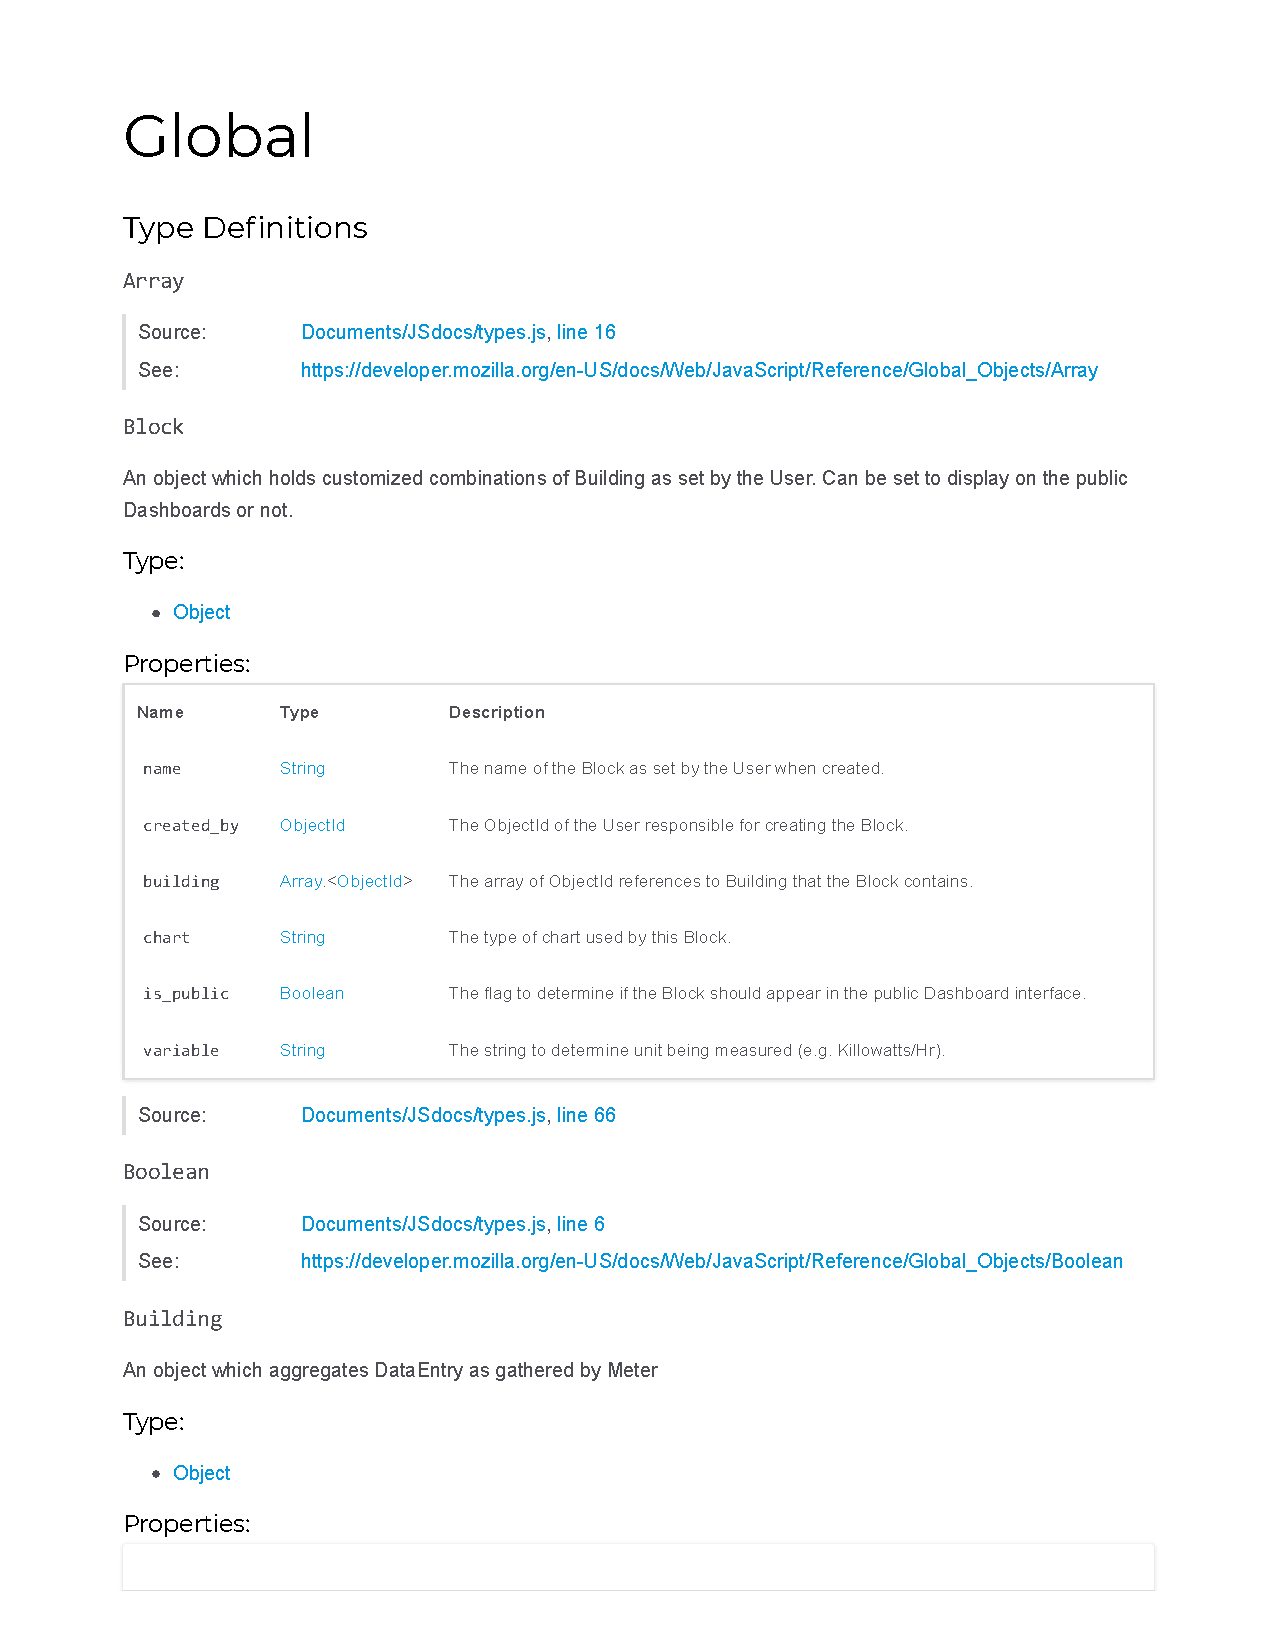
\includepdf[pages=-,scale=.95,pagecommand={}]{./pdfs/typedef.pdf}
    \subsubsection{Files}
    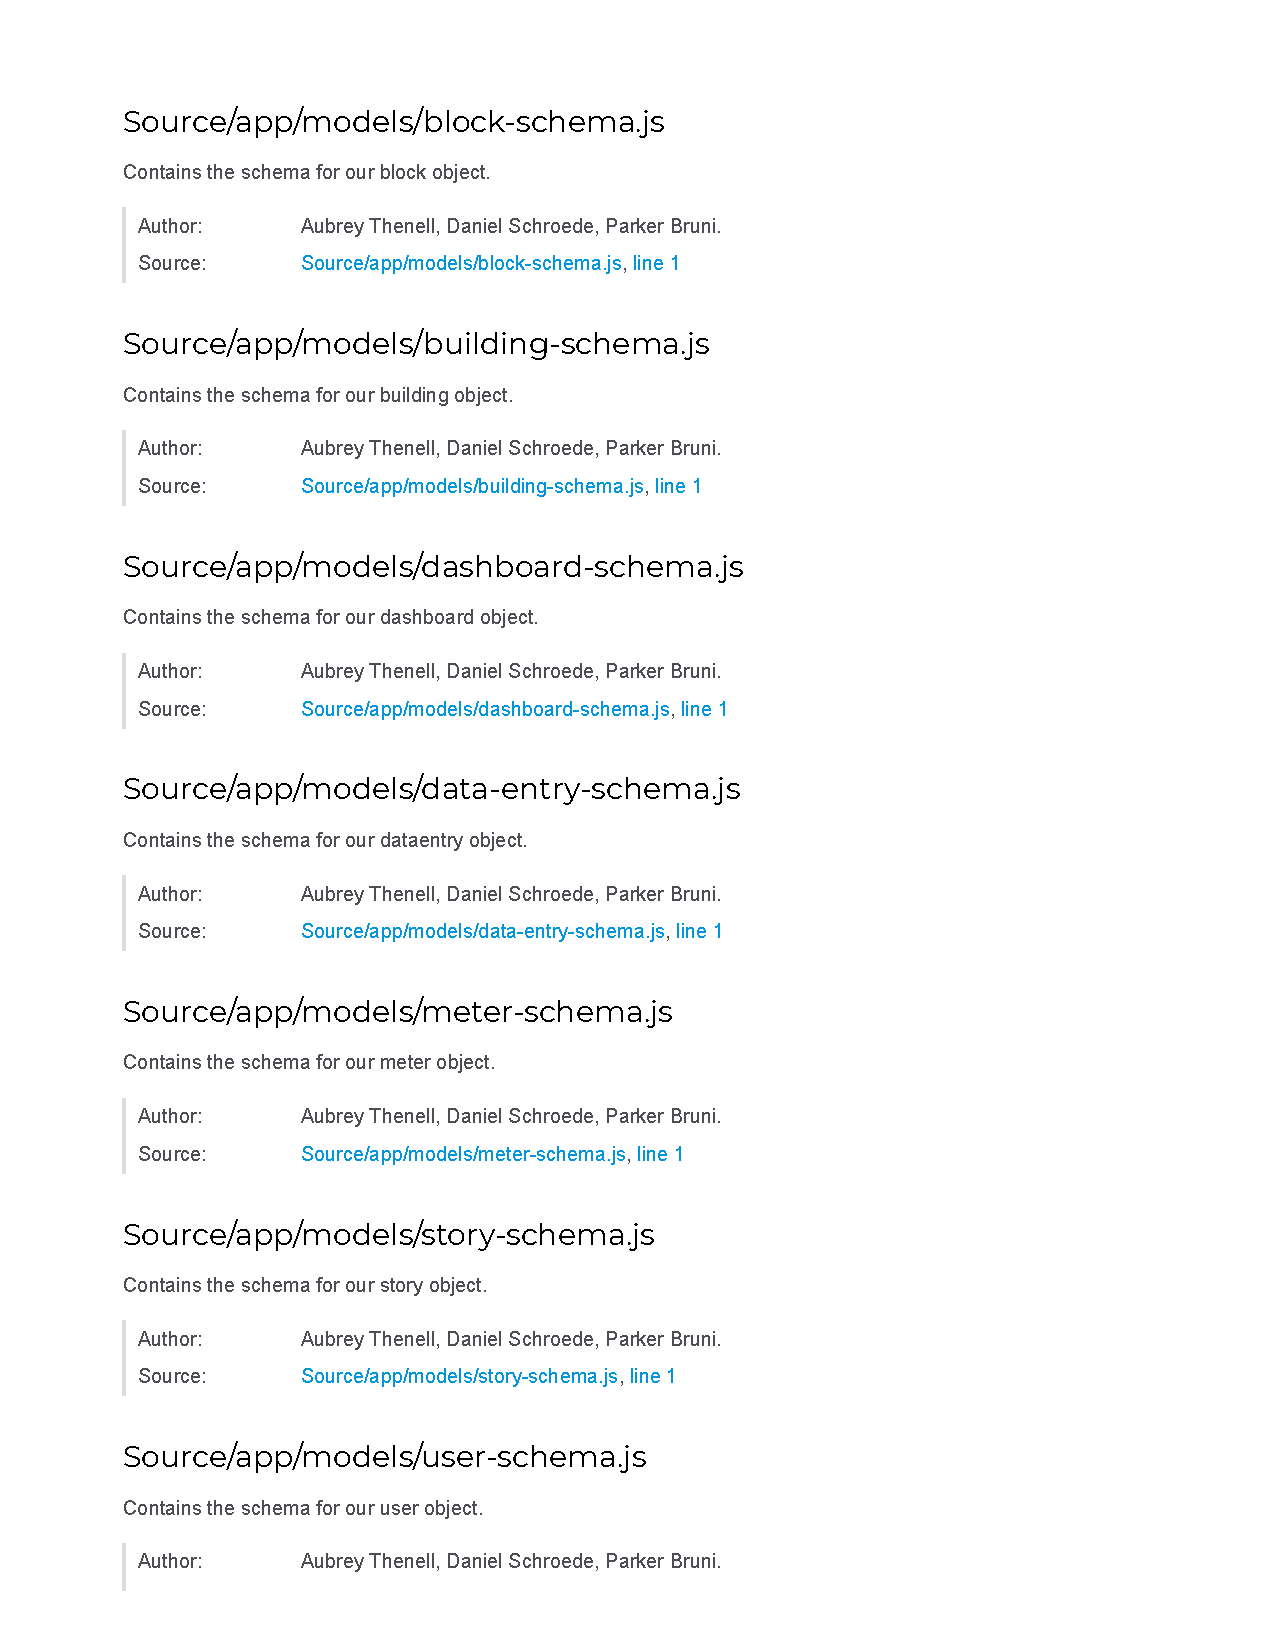
\includepdf[pages=-,scale=.95,pagecommand={}]{./pdfs/files.pdf}
    \subsubsection{DataServer}
    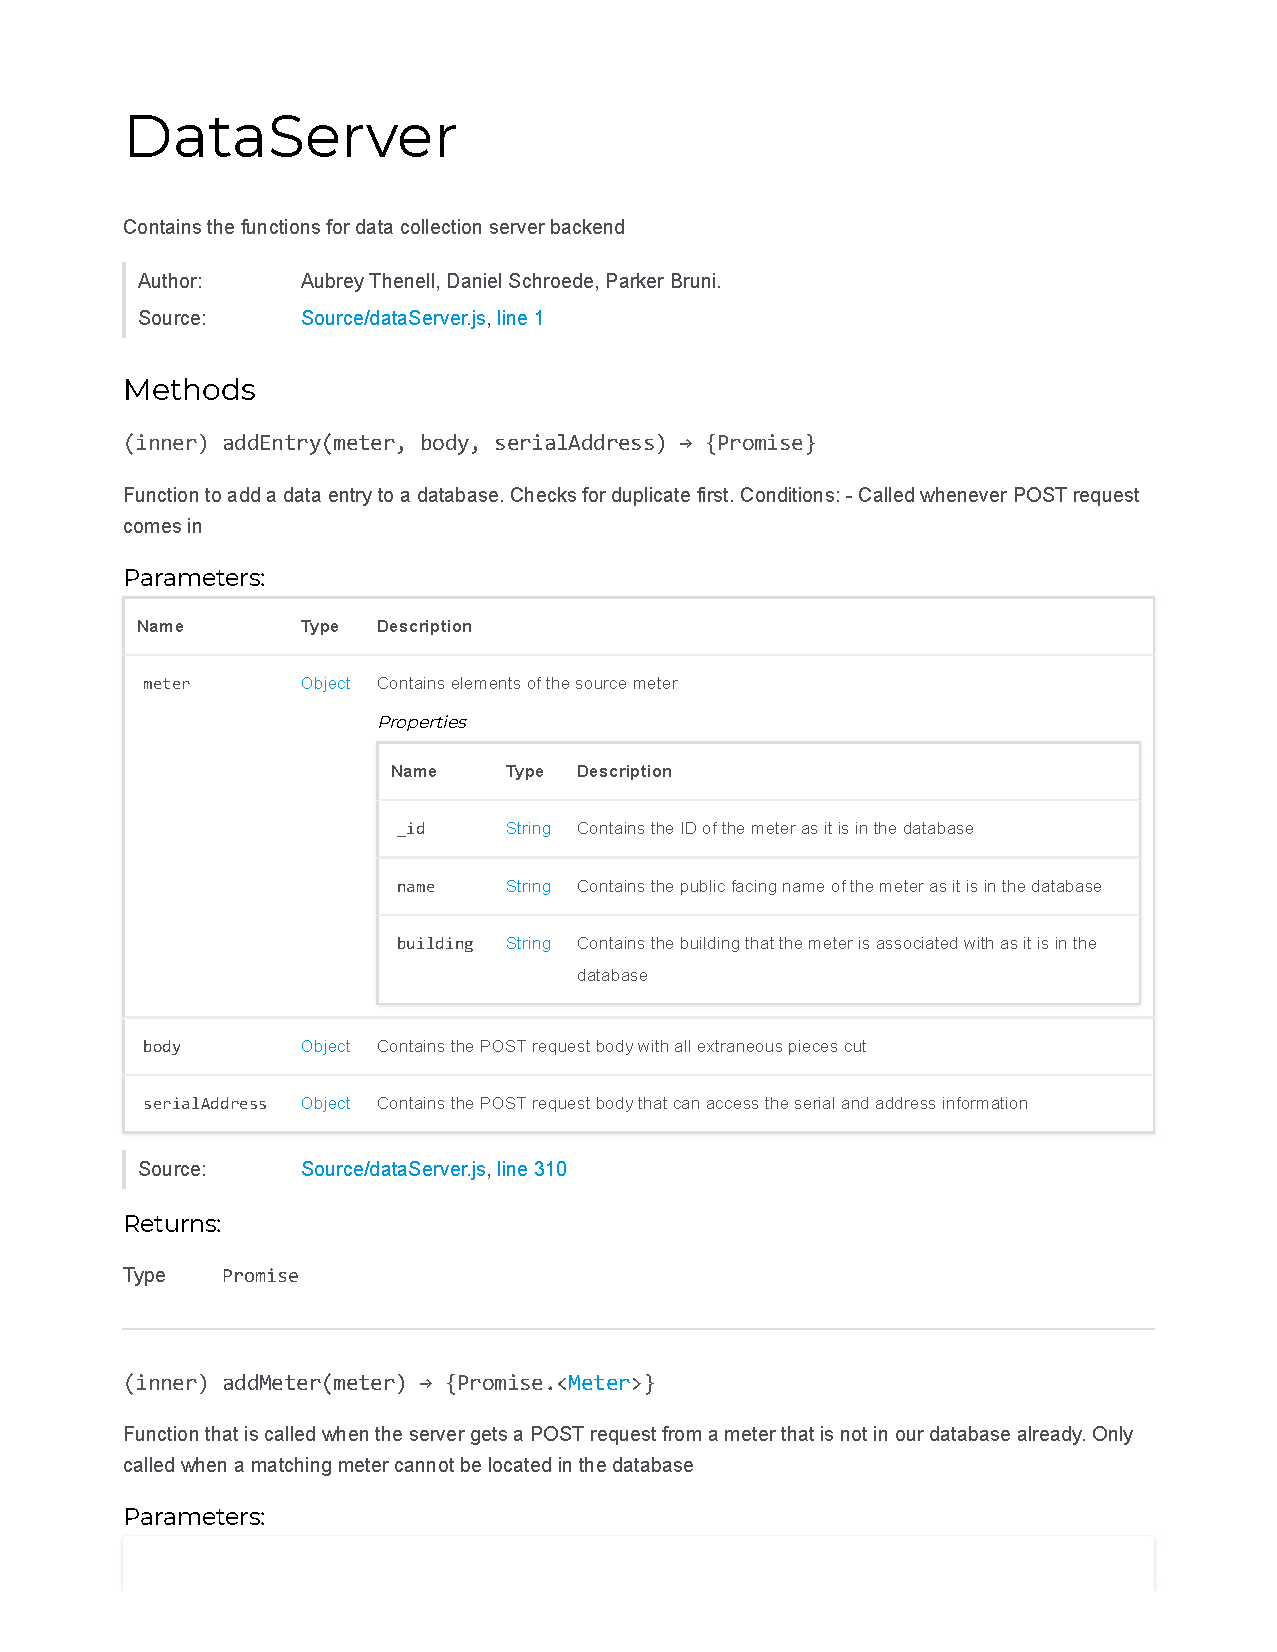
\includepdf[pages=-,scale=.95,pagecommand={}]{./pdfs/DataServer.pdf}
    \subsubsection{PublicServer}
    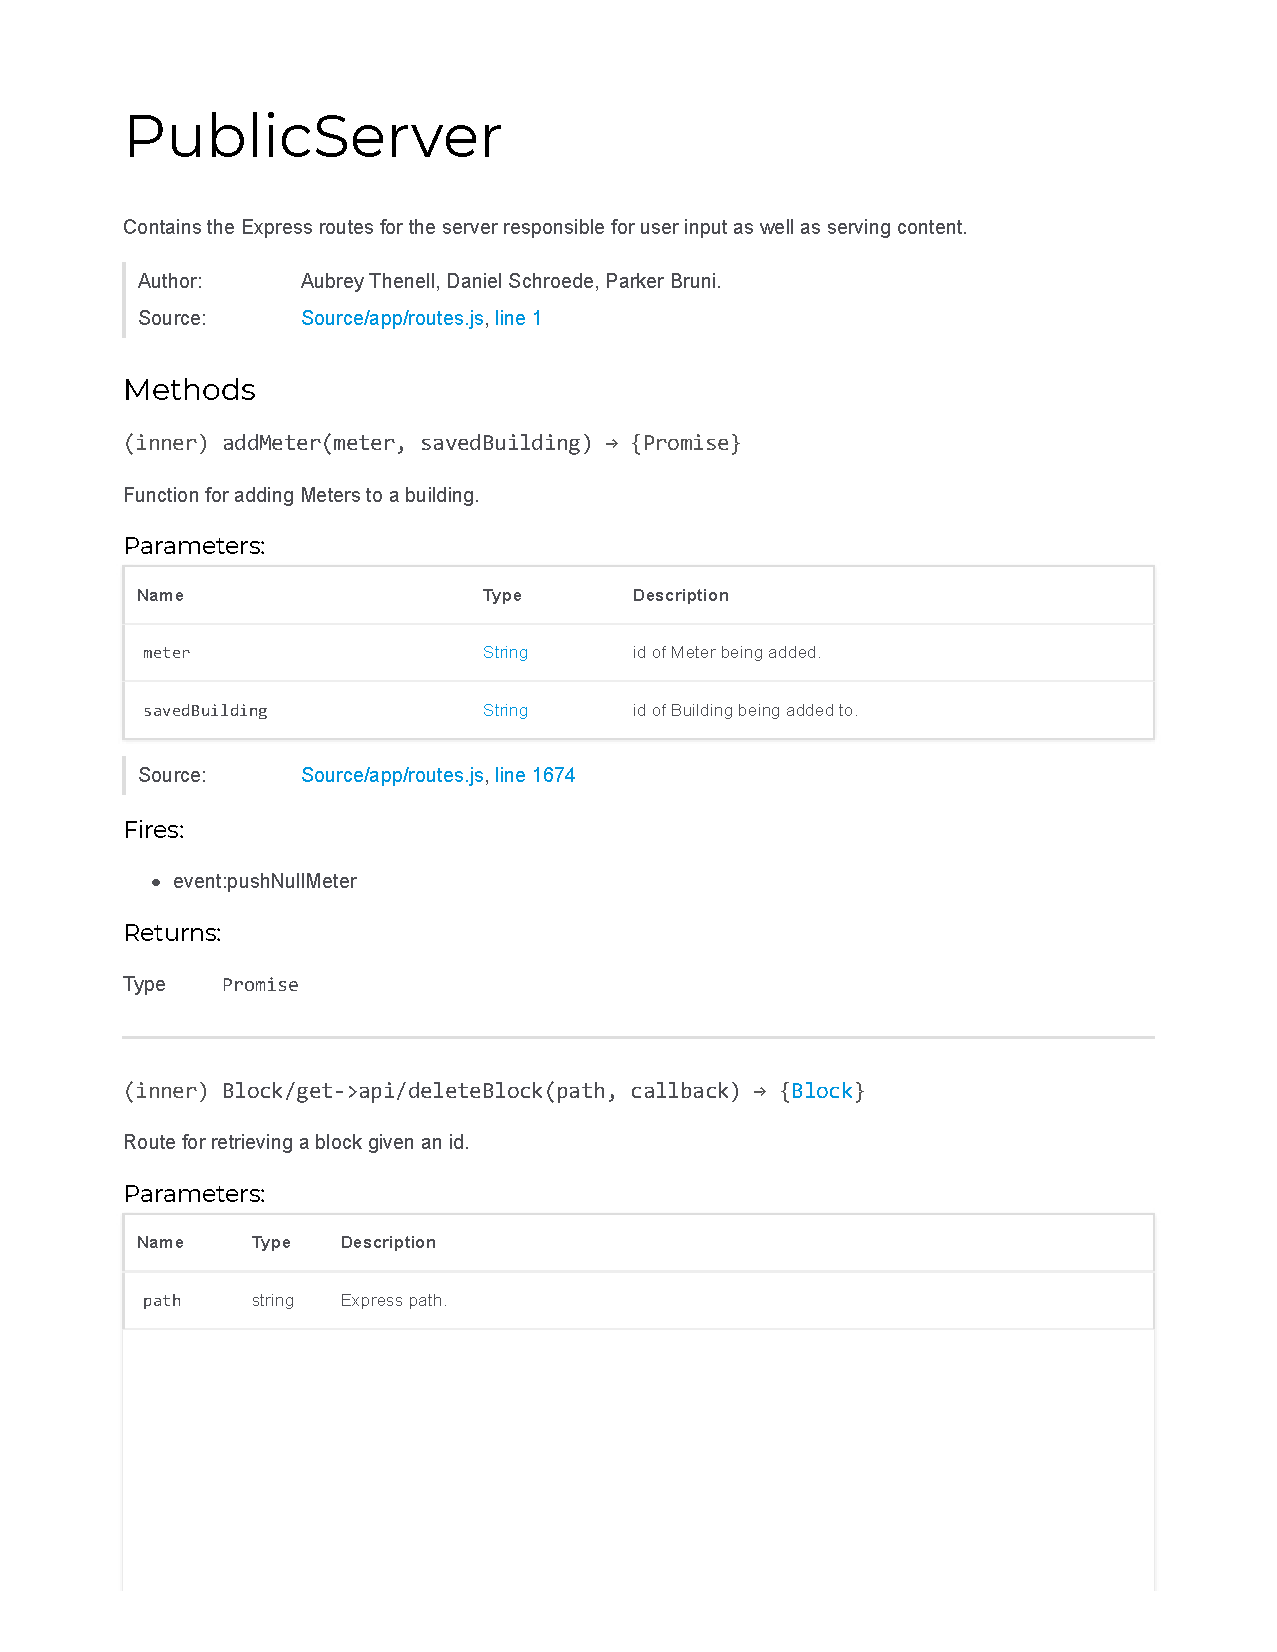
\includepdf[pages=-,scale=.95,pagecommand={}]{./pdfs/PublicServer.pdf}

    \section{Recommended Technical Resources for Learning More}
    \subsection{Helpful Websites(Listed in order of helpfulness)}
	\begin{itemize}
    \item \href{https://github.com/}{Github}
    \item \href{https://slack.com/}{Slack}
    \item \href{https://stackoverflow.com/}{Stack Overflow}
	\item \href{https://www.w3schools.com/}{W3 Schools}
    \end{itemize}
    \subsection{Helpful People on Campus}
	\begin{itemize}
    \item Kirsten Winters
    \item Kevin McGrath
	\item Behnam Saeedi
    \item Jack Woods
    \end{itemize}
    \section{Conclusions and Reflections}
    \subsection{Daniel}
    \subsubsection{What technical information did you learn?}    
    Before building this project, I had very little (if any) knowledge about AngularJS as a front-end framework, MongoDB, Amazon web services, or Express.js. While I had previously tried to do small scale M.E.A.N. stack applications, they were always bootstrapped from an example code source and I never truly understood the fundamentals behind a RESTful API or a full stack web application. I think building this project allowed me to really learn 3 main concepts:
    \begin{itemize}
        \item Read and learn from documentation
        \item Reach proficiency with the M.E.A.N. stack frameworks
        \item Understand how to design and implement a large software architecture
    \end{itemize}
    This was my first project built from scratch of something to this size and scale and it taught me a lot about the design process. I now understand why it is so common for companies to migrate legacy monolith architectures into smaller microservices. Systems that are extremely large become easily cluttered and become filled with minute work-arounds or case-dependent implementations that are not good for readability or robustness. I found that we lacked a large amount of understanding during the design process and it made a huge impact during the implementation of our project.
    \subsubsection{What non-technical information did you learn?}
    The biggest non-technical skill I learned during the course of this project was time-management and team-management. Towards the end of the project, I began setting myself hard deadlines for feature completion and implementation which proved to be extremely helpful for finishing everything that needed to get done. During the winter term, I would pick away at something here, do a little bit on something there, but never set myself deadlines for finishing up concrete requirements. I found myself becoming more and more relaxed with finishing up code and that made me fall behind at the start of spring term. I think better planning with both the architecture design and Gantt chart/read map would have proven extremely helpful throughout the development of this project.
    \subsubsection{What have you learned about project work/project management?}
    Planning and sharing work to ensure completion is crucial. Towards the end of the project, I found myself assigning personal tasks and tasks to group members with hard deadlines to speed up completion. Prior to having concrete due dates for features, the rate of implementation was slow and it seemed we were always crunched for time. I think breaking the project up into small pieces and following a concrete road map for implementations would have proven extremely helpful. 
    \subsubsection{What have you learned about working in teams?}
    I think it is important to lay out your values and expectations of yourself and others at the beginning of the project. I found that my expectations for quality and time-management differed from my group members. Putting this on the table and discussing what everyone expects from each other I think would have reduced a lot of that uncertainty and frustration throughout the year. 
    \subsubsection{If you could do it all over, what would you do differently?} 
    There are specific technical changes I would make to this project if I could do it all over again. First and foremost, for the amount of relations we had in our data, I think using MySQL as a back-end would have benefited us immensely. Secondly, and as mentioned above, I think that a thorough Gantt chart and implementation roadmap would have assisted the flow and overall quality of the project. If we had a lot of the necessary backend requirements or charting implementations done sooner, it would have alleviated a lot of the debugging and error testing that was needed towards the end of the project. I would have also like to have everyone working on and understanding every aspect of the project. Learning curves and skill-level limitations played a large role in preventing contributions in many areas of the project.
    \subsection{Parker}
    \subsubsection{What technical information did you learn?}  
	I learned a huge amount of new information on web development technologies that I had previously had no knowledge of. I learned the ins and outs of what it takes to develop a full stack web application, and while most of my efforts were on UI, I learned a decent bit about backend frameworks as well as chart.js and google maps implementations.
    \subsubsection{What non-technical information did you learn?}
	My teamwork skills have greatly improved. Specifically, communication within a team environment and the ability to adapt to different work styles to better suit the needs of the team. As well, I feel that my work ethic for large scale projects has improved. Specifically, the ability to assess requirements and the amount of work needed as well as estimating when and how much to work in order to meet deadlines. 
    \subsubsection{What have you learned about project work?}
	I know now how crucial it is to divide the work into manageable pieces between people and establish good communication between those working parties so that the project can come together as a whole in a functional format. I have previously not worked on a project of this scale for this amount of time so I have gained some good insights on how the work on a project should be handled.
    \subsubsection{What have you learned about project management?}
	I learned that a project works well when someone on the team takes the lead role, namely Daniel. This seemed to promote work ethic within the group and helped us stay organized to meet deadlines for assignments and figure out who needs to do what portions of the project and when.
    \subsubsection{What have you learned about working in teams?}
	Teamwork flows much better with good communication. The web based communication application "Slack" seemed to let us work much more efficiently as it allowed for instant text communication and file sharing. This workspace is organized with team collaboration in mind and I would recommend it to any team that is working on large scale projects. Communication is key, but so is group members who are willing and open to new ideas about changes or other aspects of the projects. In person team meetings were good to establish good relationships and in person interactions to get work done. 
    \subsubsection{If you could do it all over, what would you do differently?} 
	I would ideally know more about web based technologies, as I had a relatively small amount of knowledge of potential technologies and if I had known more potential technologies and their pros and cons we would have been able to make decisions about the project much quicker and it is likely that the final product would function more efficiently. 
    \subsection{Aubrey}
    \subsubsection{What technical information did you learn?}    
	This project has really solidified my understanding of AngularJS and related frameworks. Between this project and the projects I'm assigned at work, I am fairly solidified in what I'd like to focus on once I graduate. The most important technical takeaway is my backend knowledge. Since I focused building the backend side of the project, I have gained quite a bit of experience. This makes me happy because backend knowledge is applicable everywhere. Even if the language or framework is different, the concepts will be the same.
    \subsubsection{What non-technical information did you learn?}
	I learned that my time management has some room for improvement. Between this project, working over 20 hours a week, and taking 19 credit hours, I feel that my time management and work ethic have improved drastically over the course of the project. Another non-technical thing I learned was about energy. Through talks with Jack and the Office of Sustainability, my understanding of how sustainable systems work as well as how Oregon State University implements techniques to make itself more sustainable.
    \subsubsection{What have you learned about project work/management?}
	I think my main takeaway from this section would be to not underestimate how much time a task will take. A seemingly simple task can (and has) take dozens of hours when I only thought a few hours were needed. I also think that breaking down tasks into smaller subtasks will not only make it seem like less, but will also make it less daunting.
    \subsubsection{What have you learned about working in teams?}
	This has definitely been the most stressful group project I've done. While we got along just fine, it was rather difficult to get everyone on the same page on what needed to be done and how long dependency tasks were going to take. I think if we understood the scope of the project better from the get go, we could have worked together and figured out a better work distribution that would prevent less constant progress blocking.
    \subsubsection{If you could do it all over, what would you do differently?} 
	First and foremost I would choose the more modern Angular2+ over AngularJS. Combine this with typescript and I feel like this would have helped us keep things better modularized. I suggested Angular2+ during the design phase, but we decided to go with AngularJS because Daniel had a decent amount of experience already.  I would also want to try out SQL to see how performances differed. There were times when I was writing mongo queries that just made me wish I could use SQL queries instead. Granted, Mongo does support SQL queries, but the performance isn't as good as native SQL, so not much point using them. I would also start on the coding aspect of the project sooner. If we had a lot of the information about how the AcquiSuites worked from the get go, that would have saved me several dozen hours of debugging.
    \section{Appendix 1: Essential Code Listings.}
    
	\subsubsection{Node.js crypto salt/hash password example}
\label{sec:node_crypto}
\begin{lstlisting}[
caption={[An example of how to salt hash passwords using the Node.js crypto module]An example of how to salt hash passwords using the Node.js crypto module (Taken from \href{https://ciphertrick.com/2016/01/18/salt-hash-passwords-using-Node.js-crypto/}{\textit{Rahil Shaikh's example}})\cite{Rahil_Shaikh}}
]
'use strict';
var crypto = require('crypto');
/**
    * generates random string of characters i.e salt
    */
var genRandomString = function(length){
    return crypto.randomBytes(Math.ceil(length/2))
            .toString('hex') /** convert to hexadecimal format */
            .slice(0,length);   /** return required number of characters */
};
/** hash password with sha512.
    * @function
    * @param {string} password - List of required fields.
    * @param {string} salt - Data to be validated.
    */
var sha512 = function(password, salt){
    var hash = crypto.createHmac('sha512', salt); /** Hashing algorithm sha512 */
    hash.update(password);
    var value = hash.digest('hex');
    return {
        salt:salt,
        passwordHash:value
    };
};
function saltHashPassword(userpassword) {
    var salt = genRandomString(16); /** Gives us salt of length 16 */
    var passwordData = sha512(userpassword, salt);
    console.log('UserPassword = '+userpassword);
    console.log('Passwordhash = '+passwordData.passwordHash);
    console.log('nSalt = '+passwordData.salt);
}
\end{lstlisting}
\subsubsection{Using Passport.js to include Google oAuth 2.0 authentication}
\label{sec:passport_oauth}
\begin{lstlisting}[
caption={[Using passport to include Google oAuth 2.0 authentication]Using passport to include Google oAuth 2.0 authentication. (Taken from \href{http://www.passportjs.org/docs/username-password}{\textit{Passport Documentation}})\cite{passport_doc}}
]
var passport = require('passport');
var GoogleStrategy = require('passport-google-oauth').OAuth2Strategy;

// Use the GoogleStrategy within Passport.
//   Strategies in Passport require a `verify` function, which accept
//   credentials (in this case, an accessToken, refreshToken, and Google
//   profile), and invoke a callback with a user object.
passport.use(new GoogleStrategy({
    clientID: GOOGLE_CLIENT_ID,
    clientSecret: GOOGLE_CLIENT_SECRET,
    callbackURL: "http://www.example.com/auth/google/callback"
    },
    function(accessToken, refreshToken, profile, done) {
        User.findOrCreate({ googleId: profile.id }, function (err, user) {
            return done(err, user);
        });
    }
));
\end{lstlisting}    
\subsubsection{Using Passport.js to maintain user sessions.}
\label{sec:passport_session}
\begin{lstlisting}[
caption={[The user ID is serialized to the session, keeping the amount of data stored within the session small. When subsequent requests are received, this ID is used to find the user, which will be restored to req.user.]The user ID is serialized to the session, keeping the amount of data stored within the session small. When subsequent requests are received, this ID is used to find the user, which will be restored to req.user. (Taken from \href{http://www.passportjs.org/docs}{\textit{Passport Documentation}})\cite{passport_session}}
]
passport.serializeUser(function(user, done) {
    done(null, user.id);
    });
    
    passport.deserializeUser(function(id, done) {
    User.findById(id, function(err, user) {
        done(err, user);
    });
    });
\end{lstlisting}

\subsubsection{Using UI Bootstrap to create a datepicker object.}
\label{sec:ui_bootstrap}
\begin{lstlisting}[
    caption={[An example of using UI Bootstrap to create a datepicker object with an Angular controller.]An example of using UI Bootstrap to create a datepicker object with an Angular controller. (Taken from \href{https://codepen.io/joe-watkins/pen/KsAgp}{\textit{Angular - Bootstrap UI - Datepicker}})\cite{Watkins}}
    ]
    // HTML Declaration
    <input type="text" class="form-control" 
        datepicker-popup="{{format}}" 
        ng-model="dt" 
        is-open="opened" 
        min-date="minDate" 
        max-date="'2015-06-22'"
        datepicker-options="dateOptions" 
        date-disabled="disabled(date, mode)" 
        ng-required="true" 
        close-text="Close" 
        id="date-picker" 
        readonly
        ng-click="open($event)"
    />
    
    // Angular Controller
    var calPicker = angular.module("calPicker", ['ui.bootstrap']);
    
    calPicker.controller("DatepickerDemoCtrl", ["$scope", function($scope){
        
        // grab today and inject into field
        $scope.today = function() {
        $scope.dt = new Date();
        };
        
        // run today() function
        $scope.today();
    
        // setup clear
        $scope.clear = function () {
        $scope.dt = null;
        };
    
        // open min-cal
        $scope.open = function($event) {
        $event.preventDefault();
        $event.stopPropagation();
    
        $scope.opened = true;
        };
        
        // handle formats
        $scope.formats = ['dd-MMMM-yyyy', 'yyyy/MM/dd', 'dd.MM.yyyy', 'shortDate'];
        
        // assign custom format
        $scope.format = $scope.formats[0];
        
    }]);
    \end{lstlisting}
    
    \section{Appendix 2: Anything else you want to include.}
    Photos, etc.
    \subsection{Design Document Images}
\subsubsection{Home Webpage (Public Access)}
\label{sec:home_public}
\begin{figure}[H]
    \centering
    \includegraphics[width=14cm]{images/Home_NOT_Logged_In.eps}
    \caption{A mock-up of a home page from a general public user access perspective (not logged in to an account).}
\end{figure}

\subsubsection{Home Webpage (Logged in Access)}
\label{sec:home_logged}
\begin{figure}[H]
    \centering
    \includegraphics[width=14cm]{images/Home_Logged_In.eps}
    \caption{A mock-up of a home page from an authorized user access perspective (logged in to an account).}
\end{figure}

\subsubsection{Buildings Webpage}
\label{sec:buildings}
\begin{figure}[H]
    \centering
    \includegraphics[width=14cm]{images/buildings.eps}
    \caption{A mock-up of the webpage that shows all buildings.}
\end{figure}

\subsubsection{Selected Building Page}
\label{sec:selected_buildings}
\begin{figure}[H]
    \centering
    \includegraphics[width=14cm]{images/Building_Select.eps}
    \caption{A mock-up of a selected building page.}
\end{figure}


\subsubsection{Dashboards Page}
\label{sec:dashboards}
\begin{figure}[H]
    \centering
    \includegraphics[width=14cm]{images/Dashboards.eps}
    \caption{A mock-up page of a list of user generated dashboards.}
\end{figure}

\subsubsection{Selected Dashboard Webpage}
\label{sec:selected_dashboards}
\begin{figure}[H]
    \centering
    \includegraphics[width=14cm]{images/Dashboard_Select.eps}
    \caption{A mock-up of a selected dashboard webpage.}
\end{figure}

\subsubsection{Stories Webpage}
\label{sec:story}
\begin{figure}[H]
    \centering
    \includegraphics[width=14cm]{images/Stories.eps}
    \caption{A mock-up of a list of user generated story Webpages.}
\end{figure}

\subsection{Technology Review Images}
    \pagebreak
    \bibliographystyle{IEEEtran}
    \bibliography{refs}
    \end{document}